\documentclass[a4paper,11pt]{book}

\author{Sebastian Pancratz}
\title{Practical improvements to the deformation method for point counting}

%%%%%%%%%%%%%%%%%%%%%%%%%%%%%%%%%%%%%%%%%%%%%%%%%%%%%%%%%%%%%%%%%%%%%%%%%%%%%%%
% Geometry and page layout

\usepackage[hmargin=2.2cm,vmargin=3cm,a4paper,centering,twoside]{geometry}

\setlength{\headheight}{14pt}

%%%%%%%%%%%%%%%%%%%%%%%%%%%%%%%%%%%%%%%%%%%%%%%%%%%%%%%%%%%%%%%%%%%%%%%%%%%%%%%
% Other packages

\usepackage{ifpdf}
\usepackage{paralist}
\usepackage{fancyhdr}
\usepackage{sectsty}
\usepackage{natbib}
\usepackage{url}
\usepackage[T1]{fontenc}
\usepackage{ae,aecompl}
\usepackage{booktabs}
\usepackage{multirow}
\usepackage{verbatim}

\usepackage{float}
\usepackage{tikz}
\usetikzlibrary{shapes,arrows}

%%%%%%%%%%%%%%%%%%%%%%%%%%%%%%%%%%%%%%%%%%%%%%%%%%%%%%%%%%%%%%%%%%%%%%%%%%%%%%%
% hyperref

\usepackage{hyperref}
\hypersetup{
    colorlinks=true,    % false: boxed links; true: colored links
    citecolor=green,    % color of links to bibliography
    filecolor=magenta,  % color of file links
    linkcolor=red,      % color of internal links
    urlcolor=blue       % color of external links
}

\makeatletter
\newcommand\org@hypertarget{}
\let\org@hypertarget\hypertarget
\renewcommand\hypertarget[2]{%
    \Hy@raisedlink{\org@hypertarget{#1}{}}#2%
} 
\makeatother

\ifpdf
    \hypersetup{
        pdftitle={Deformation method},
        pdfauthor={Sebastian Pancratz},
        pdfsubject={Computational Number Theory},
        bookmarks=true,
        bookmarksnumbered=true,
        unicode=true,
        pdfstartview={FitH},
        pdfpagemode={UseOutlines}
    }
\fi

%%%%%%%%%%%%%%%%%%%%%%%%%%%%%%%%%%%%%%%%%%%%%%%%%%%%%%%%%%%%%%%%%%%%%%%%%%%%%%%
% natbib

\bibpunct{[}{]}{,}{n}{}{}
%\bibpunct{[}{]}{;}{a}{,}{,}

%%%%%%%%%%%%%%%%%%%%%%%%%%%%%%%%%%%%%%%%%%%%%%%%%%%%%%%%%%%%%%%%%%%%%%%%%%%%%%%
% sectsty

\allsectionsfont{\nohang\centering}

%%%%%%%%%%%%%%%%%%%%%%%%%%%%%%%%%%%%%%%%%%%%%%%%%%%%%%%%%%%%%%%%%%%%%%%%%%%%%%%
% fancyhdr

\newcommand\nouppercase[1]{{%
    \let\uppercase\relax
    \let\MakeUppercase\relax
    \expandafter\let\csname MakeUppercase \endcsname\relax#1}%
}

\pagestyle{fancyplain}

\renewcommand{\chaptermark}[1]{\markboth{#1}{}}
\renewcommand{\sectionmark}[1]{\markright{\thesection\ #1}}
\fancyhf{}
\fancyhead[LE,RO]{\bfseries\thepage}
\fancyhead[LO]{\itshape\nouppercase{\rightmark}}
\fancyhead[RE]{\itshape\nouppercase{\leftmark}}
\renewcommand{\headrulewidth}{0pt}
\renewcommand{\footrulewidth}{0pt}

\fancypagestyle{plain}{%
  \fancyhead{}
  \renewcommand{\headrulewidth}{0pt}
}

\makeatletter
\def\cleardoublepage{\clearpage\if@twoside \ifodd\c@page\else
    \hbox{}
    \thispagestyle{plain}
    \newpage
    \if@twocolumn\hbox{}\newpage\fi\fi\fi}
\makeatother \clearpage{\pagestyle{plain}\cleardoublepage}

%%%%%%%%%%%%%%%%%%%%%%%%%%%%%%%%%%%%%%%%%%%%%%%%%%%%%%%%%%%%%%%%%%%%%%%%%%%%%%%
% url

\makeatletter
\def\url@leostyle{%
  \@ifundefined{selectfont}{\def\UrlFont{\sf}}{\def\UrlFont{\small\ttfamily}}}
\makeatother
\urlstyle{leostyle}

%%%%%%%%%%%%%%%%%%%%%%%%%%%%%%%%%%%%%%%%%%%%%%%%%%%%%%%%%%%%%%%%%%%%%%%%%%%%%%%
% Enumeration

\setlength{\pltopsep}{0.24em}
\setlength{\plpartopsep}{0em}
\setlength{\plitemsep}{0.24em}

% This should do what we want
%   \setdefaultenum{(i)}{(a)}{1.}{A}
% but it does not work for references, dropping the parentheses.  The following
% hack does work.

\renewcommand{\theenumi}{(\roman{enumi})}
\renewcommand{\theenumii}{(\alph{enumii})}
\renewcommand{\theenumiii}{\arabic{enumiii}.}
\renewcommand{\theenumiv}{\Alph{enumiv}}

\renewcommand{\labelenumi}{\theenumi}
\renewcommand{\labelenumii}{\theenumii}
\renewcommand{\labelenumiii}{\theenumiii}
\renewcommand{\labelenumiv}{\theenumiv}

%%%%%%%%%%%%%%%%%%%%%%%%%%%%%%%%%%%%%%%%%%%%%%%%%%%%%%%%%%%%%%%%%%%%%%%%%%%%%%%
% Bibliography name

\renewcommand{\bibname}{References}

%%%%%%%%%%%%%%%%%%%%%%%%%%%%%%%%%%%%%%%%%%%%%%%%%%%%%%%%%%%%%%%%%%%%%%%%%%%%%%%
% Mathematical definitions

%%%%%%%%%%%%%%%%%%%%%%%%%%%%%%%%%%%%%%%%%%%%%%%%%%%%%%%%%%%%%%%%%%%%%%%%%%%%%%%
% A selection of mathematical commands for inclusion in a LaTeX document.
% 
% Author.  Sebastian Pancratz
% Date.    Nov 2009

%%%%%%%%%%%%%%%%%%%%%%%%%%%%%%%%%%%%%%%%%%%%%%%%%%%%%%%%%%%%%%%%%%%%%%%%%%%%%%%
% Packages

\usepackage{amsmath,amsthm,amscd,amsfonts,amssymb}
\usepackage{cases}
\usepackage[all]{xy}

%%%%%%%%%%%%%%%%%%%%%%%%%%%%%%%%%%%%%%%%%%%%%%%%%%%%%%%%%%%%%%%%%%%%%%%%%%%%%%%
% General Mathematics

\newcommand{\myland}{\mspace{6mu} \land \mspace{6mu}}%  logical and
\newcommand{\mylor}{\mspace{6mu} \lor \mspace{6mu}}%    logical or

\renewcommand{\to}{\rightarrow}%           Right arrow
\newcommand{\into}{\hookrightarrow}%     Injection arrow
\newcommand{\onto}{\twoheadrightarrow}%  Surjection arrow

\providecommand{\card}[1]{\left\lvert#1\right\rvert}%    Cardinality
\providecommand{\cardts}[1]{\lvert#1\rvert}%             Cardinality
\providecommand{\cardbig}[1]{\bigl\lvert#1\bigr\rvert}%  Cardinality

\providecommand{\abs}[1]{\lvert#1\rvert}%                  Absolute value
\providecommand{\absbig}[1]{\bigl\lvert#1\bigr\rvert}%     Absolute value
\providecommand{\absBig}[1]{\Bigl\lvert#1\Bigr\rvert}%     Absolute value
\providecommand{\absbigg}[1]{\biggl\lvert#1\biggr\rvert}%  Absolute value

\providecommand{\norm}[1]{\lVert#1\rVert}%               Norm
\providecommand{\normbig}[1]{\bigl\lVert#1\bigr\rVert}%  Norm
\providecommand{\normBig}[1]{\Bigl\lVert#1\Bigr\rVert}%  Norm

\providecommand{\floor}[1]{\left\lfloor#1\right\rfloor}%    Floor
\providecommand{\floorts}[1]{\lfloor#1\rfloor}%             Floor
\providecommand{\floorbig}[1]{\bigl\lfloor#1\bigr\rfloor}%  Floor
\providecommand{\floorBig}[1]{\Bigl\lfloor#1\Bigr\rfloor}%  Floor

\providecommand{\ceil}[1]{\left\lceil#1\right\rceil}%  Ceiling

\providecommand{\id}{\iota}%              Identity element or function
\DeclareMathOperator{\ind}{1}%            Indicator function
\DeclareMathOperator{\indf}{\mathbf{1}}%  Indicator function

\DeclareMathOperator{\fCoKer}{coker}%  Cokernel
\DeclareMathOperator{\fKer}{ker}%      Kernel
\DeclareMathOperator{\fIm}{Im}%        Image

\DeclareMathOperator{\Comb}{C}%  Combinations
\DeclareMathOperator{\Perm}{P}%  Permutations

%%%%%%%%%%%%%%%%%%%%%%%%%%%%%%%%%%%%%%%%%%%%%%%%%%%%%%%%%%%%%%%%%%%%%%%%%%%%%%%
% Commonly used Sets

\newcommand{\N}{\mathbf{N}}%  Natural numbers
\newcommand{\Z}{\mathbf{Z}}%  Integers
\newcommand{\Q}{\mathbf{Q}}%  Rationals
\newcommand{\A}{\mathbf{A}}%  Algebraic numbers
\newcommand{\R}{\mathbf{R}}%  Real numbers
\providecommand{\C}{\mathbf{C}}%  Complex numbers
\newcommand{\F}{\mathbf{F}}%  Finite field

\let\P=\undefined
\newcommand{\P}{\mathbf{P}}%  Projective space, N.B.  Clashes with Probability

%%%%%%%%%%%%%%%%%%%%%%%%%%%%%%%%%%%%%%%%%%%%%%%%%%%%%%%%%%%%%%%%%%%%%%%%%%%%%%%
% Probability

%\let\P=\undefined

\DeclareMathOperator{\E}{\mathbb{E}}%  Expectation
%\DeclareMathOperator{\P}{\mathbb{P}}%  Probability
\DeclareMathOperator{\Var}{Var}%       Variance
\DeclareMathOperator{\Cov}{Cov}%       Covariance
\DeclareMathOperator{\Corr}{Corr}%     Correlation

%%%%%%%%%%%%%%%%%%%%%%%%%%%%%%%%%%%%%%%%%%%%%%%%%%%%%%%%%%%%%%%%%%%%%%%%%%%%%%%
% Algebraic Topology

\DeclareMathOperator{\rel}{rel}
\providecommand{\GeoReal}[1]{\abs{#1}}
\DeclareMathOperator{\Star}{star}
\DeclareMathOperator{\mesh}{mesh}

%%%%%%%%%%%%%%%%%%%%%%%%%%%%%%%%%%%%%%%%%%%%%%%%%%%%%%%%%%%%%%%%%%%%%%%%%%%%%%%
% Complex Analysis

\providecommand{\wn}{\omega}%  Winding number

%%%%%%%%%%%%%%%%%%%%%%%%%%%%%%%%%%%%%%%%%%%%%%%%%%%%%%%%%%%%%%%%%%%%%%%%%%%%%%%
% Galois Theory

\DeclareMathOperator{\Disc}{Disc}%      Discriminant
\DeclareMathOperator{\ch}{char}%        Characteristic
\DeclareMathOperator{\geomCirc}{circ}%  Circle for ruler & compass constructions
\DeclareMathOperator{\Gal}{Gal}%        Galois group

%%%%%%%%%%%%%%%%%%%%%%%%%%%%%%%%%%%%%%%%%%%%%%%%%%%%%%%%%%%%%%%%%%%%%%%%%%%%%%%
% Graph Theory

\providecommand{\E}{\mathbb{E}}%  Edge space
\providecommand{\V}{\mathbb{V}}%  Vertex space
\DeclareMathOperator{\ex}{ex}%    Maximal size of a graph such that it does not have a given subgraph

%%%%%%%%%%%%%%%%%%%%%%%%%%%%%%%%%%%%%%%%%%%%%%%%%%%%%%%%%%%%%%%%%%%%%%%%%%%%%%%
% Groups, Rings and Modules

\providecommand{\subgrp}{\leq}%           Subgroup
\providecommand{\normal}{\triangleleft}%  Normal subgroup
\providecommand{\subring}{\leq}%          Subring
\providecommand{\ideal}{\triangleleft}%   Ideal
\providecommand{\submodule}{\leq}%        Submodule

\DeclareMathOperator{\Sym}{Sym}%      Symmetric group
\DeclareMathOperator{\Aut}{Aut}%      Automorphism group
\DeclareMathOperator{\ccl_G}{ccl_G}%  Conjugacy class
\DeclareMathOperator{\Ann}{Ann}%      Annihilator
\DeclareMathOperator{\sgn}{sgn}%      Sign, signature
\DeclareMathOperator{\stab}{Stab}%    Stabiliser

%%%%%%%%%%%%%%%%%%%%%%%%%%%%%%%%%%%%%%%%%%%%%%%%%%%%%%%%%%%%%%%%%%%%%%%%%%%%%%%
% Linear Algebra, Linear Analysis

\providecommand{\vect}[1]{\mathbf{#1}}%                       Vector
\providecommand{\vspan}[1]{\langle #1 \rangle}%               Span
\providecommand{\iprod}[2]{\langle #1,#2 \rangle}%            Inner product
\providecommand{\ip}[2]{\left\langle #1 , #2 \right\rangle}%  Inner product

\DeclareMathOperator{\rank}{rank}%       Rank of a matrix
\DeclareMathOperator{\vsspan}{span}%     Span
\DeclareMathOperator{\diag}{diag}%       Diagonal matrix
\DeclareMathOperator{\rowrank}{rowrk}%   Row rank
\DeclareMathOperator{\colspace}{colsp}%  Column space
\DeclareMathOperator{\rowspace}{rowsp}%  Column space
\DeclareMathOperator{\adj}{adj}%         Adjoint matrix
\DeclareMathOperator{\trace}{tr}%        Trace
\DeclareMathOperator{\End}{End}%         Space of endomorphisms
\DeclareMathOperator{\SL}{SL}%           Special linear group of matrices

%%%%%%%%%%%%%%%%%%%%%%%%%%%%%%%%%%%%%%%%%%%%%%%%%%%%%%%%%%%%%%%%%%%%%%%%%%%%%%%
% Metric and Topological Spaces

\DeclareMathOperator{\diam}{diam}%  Diameter
\DeclareMathOperator{\Int}{int}%    Interior of a set
\DeclareMathOperator{\Cl}{cl}%      Closure of a set

%%%%%%%%%%%%%%%%%%%%%%%%%%%%%%%%%%%%%%%%%%%%%%%%%%%%%%%%%%%%%%%%%%%%%%%%%%%%%%%
% Number Theory

\providecommand{\jacobi}[2]{\left( \frac{#1}{#2} \right)}%    Jacobi symbol (display)
\providecommand{\jacobii}[2]{\left( #1 \vert #2 \right)}%     Jacobi symbol (inline)
\providecommand{\legendre}[2]{\left( \frac{#1}{#2} \right)}%  Legendre symbol (display)
\providecommand{\legendrei}[2]{\left( #1 \vert #2 \right)}%   Legendre symbol (inline)

\DeclareMathOperator{\hcf}{hcf}%  Highest common factor
\DeclareMathOperator{\lcm}{lcm}%  Lowest common multiple

%%%%%%%%%%%%%%%%%%%%%%%%%%%%%%%%%%%%%%%%%%%%%%%%%%%%%%%%%%%%%%%%%%%%%%%%%%%%%%%
% Local Fields

\newcommand{\ilim}{\varprojlim}%  inverse limit

\DeclareMathOperator{\ord}{ord}%          Valuation
\DeclareMathOperator{\Frac}{Frac}%        Field of fractions
\DeclareMathOperator{\Frob}{\mathcal{F}}% Frobenius map
\DeclareMathOperator{\Hom}{Hom}%          Space of homomorphisms
\DeclareMathOperator{\Tr}{Tr}%            Trace

%%%%%%%%%%%%%%%%%%%%%%%%%%%%%%%%%%%%%%%%%%%%%%%%%%%%%%%%%%%%%%%%%%%%%%%%%%%%%%%
% Algebraic Geometry

\DeclareMathOperator{\Spec}{Spec}%  Spectrum

%%%%%%%%%%%%%%%%%%%%%%%%%%%%%%%%%%%%%%%%%%%%%%%%%%%%%%%%%%%%%%%%%%%%%%%%%%%%%%%
% Calligraphic letters

\providecommand{\cB}{\mathcal{B}}%   Basis, factor base
\providecommand{\fC}{\mathfrak{C}}%  Codes
\providecommand{\cS}{\mathcal{S}}%   Signatures
\providecommand{\cK}{\mathfrak{K}}%  Keys
\providecommand{\cM}{\mathfrak{M}}%  Messages
\providecommand{\cE}{\mathcal{E}}%   (See error locator polynomial)
\providecommand{\cF}{\mathcal{F}}%   Family
\providecommand{\cO}{\mathcal{O}}%   Big-oh notation
\providecommand{\cP}{\mathcal{P}}%   Power set
\providecommand{\cR}{\mathcal{R}}%   Row index set
\providecommand{\cC}{\mathcal{C}}%   Column index set


%%%%%%%%%%%%%%%%%%%%%%%%%%%%%%%%%%%%%%%%%%%%%%%%%%%%%%%%%%%%%%%%%%%%%%%%%%%%%%%
% Equations

\allowdisplaybreaks[4]
\numberwithin{equation}{chapter}

%%%%%%%%%%%%%%%%%%%%%%%%%%%%%%%%%%%%%%%%%%%%%%%%%%%%%%%%%%%%%%%%%%%%%%%%%%%%%%%
% Theorems etc

\theoremstyle{definition}

\newtheorem{thm}{Theorem}[section]
\newtheorem{lem}[thm]{Lemma}
\newtheorem{prop}[thm]{Proposition}
\newtheorem{cor}[thm]{Corollary}
\newtheorem{defn}[thm]{Definition}
\newtheorem{exmp}[thm]{Example}
\newtheorem{rem}[thm]{Remark}
\newtheorem{assumption}[thm]{Assumption}
\newtheorem{notation}[thm]{Notation}
\newtheorem{prob}[thm]{Problem}
\newtheorem{obs}[thm]{Observation}

%%%%%%%%%%%%%%%%%%%%%%%%%%%%%%%%%%%%%%%%%%%%%%%%%%%%%%%%%%%%%%%%%%%%%%%%%%%%%%%
% DOCUMENT                                                                    %
%%%%%%%%%%%%%%%%%%%%%%%%%%%%%%%%%%%%%%%%%%%%%%%%%%%%%%%%%%%%%%%%%%%%%%%%%%%%%%%

\begin{document}

\frontmatter

\tableofcontents

\mainmatter

{%
\part{The deformation method}
\setlength{\baselineskip}{1.5\baselineskip}
%%%%%%%%%%%%%%%%%%%%%%%%%%%%%%%%%%%%%%%%%%%%%%%%%%%%%%%%%%%%%%%%%%%%%%%%%%%%%%%
% Introduction to point counting                                              %
%%%%%%%%%%%%%%%%%%%%%%%%%%%%%%%%%%%%%%%%%%%%%%%%%%%%%%%%%%%%%%%%%%%%%%%%%%%%%%%

\chapter{Introduction to point counting}

% Chapter:  Introduction to point counting  %%%%%%%%%%%%%%%%%%%%%%%%%%%%%%%%%%%

% Varieties over finite fields and zeta functions %%%%%%%%%%%%%%%%%%%%%%%%%%%%%

\section{Varieties over finite fields and zeta functions}

Let $X$ denote an algebraic variety over the finite field~$\mathbf{F}_q$ 
with $q = p^a$ elements.  In particular, $X$ is also defined 
over every algebraic extension $\mathbf{F}_{q^i}$, for $i \geq 0$, 
and we can let $N_i = \abs{ X(\mathbf{F}_{q^i}) }$ denote the number 
of points of $X$ over $\mathbf{F}_{q^i}$.  The \emph{zeta function} 
of $X$ is then defined as the formal power series in $\mathbf{Q}[[T]]$,
\begin{equation*}
Z(X, T) = \exp \Bigl( \sum_{i=0}^{\infty} \frac{N_i T^i}{i} \Bigr).
\end{equation*}
In the above form, the power series~$Z(X, T)$ is represented by an 
infinite series and it is unclear whether this can be explicitly 
computed by an algorithm viz.\ a \emph{finite} routine.  This issue 
was resolved by Dwork~\citep{Dwork1960} in 1960:

\begin{thm}
Let $X$ be an algebraic variety over the finite field~$\mathbf{F}_q$.  
Then the zeta function $Z(X, T)$ is a quotient of two polynomials with 
integer coefficients.
\end{thm}

Moreover, Bombieri~\citep{Bombieri1978} provided an explicit bound 
for the total degree of the rational function representing $Z(X, T)$.
Dwork's theorem is included in a group of results known as the 
\emph{Weil conjectures}, statements conjectured by Weil~\citep{Weil1949} 
in~1949 which have subsequently been proved by Dwork, Grothendieck, 
Deligne, et al.\ (see~\citep[Appendix~C]{Har77}).  We follow 
Kedlaya~\citep[Theorem~1.2.1]{Kedlaya2011} in the statement of the Weil 
conjectures:

\begin{thm} \label{thm:01-Zetafunctions}
Let $X$ be a separated scheme of finite type over the finite 
field~$\mathbf{F}_q$.  Then the zeta function of~$X$ is the power series 
representation of a rational function~$T$.  Moreover, if $X$ is smooth 
and proper over~$\mathbf{F}_q$, then there is a unique way to write 
\begin{equation}
Z(X, T) = \prod_{i=0}^{2 \dim(X)} P_i(T)^{(-1)^{i+1}}
\end{equation}
for some polynomials $P_i(T) \in \mathbf{Z}[T]$ with $P_i(0) = 1$, 
satisfying the following conditions.
\begin{enumerate}
\item We have 
\begin{equation*}
P_i(q^{-i} / T) = \pm q^{-i \deg(P_i) / 2} T^{- \deg(P_i)} P_i(T),
\end{equation*}
with the sign being $+$ whenever $i$ is odd.  In other words, the roots 
of~$P_i$ are invariant under the map $r \mapsto q^{-i} / r$, and if $i$ 
is odd then the multiplicities of $\pm q^{-i/2}$ are even.
\item The complex roots of $P_i$ all have absolute value $q^{-i/2}$.
\item If $X \cong \mathfrak{X}_{\mathbf{F}_q}$ for some smooth proper 
scheme~$\mathfrak{X}$ over the local ring $R = \mathfrak{o}_{K,\mathfrak{p}}$, 
for some number field~$K$ and some prime ideal~$\mathfrak{p}$ of 
$\mathfrak{o}_K$ with residue field~$\mathbf{F}_q$, then for any 
embedding~$K \into \mathbf{C}$, 
\begin{equation*}
\deg(P_i) = \dim_{\mathbf{C}} H^{i} \bigl( (\mathfrak{X} \times_R \mathbf{C})^{\text{an}}, \mathbf{C} \bigr).
\end{equation*}
In other words, $\deg(P_i)$ equals the $i$-th Betti number of 
$\mathfrak{X} \times_{R} \mathbf{C}$.
\end{enumerate}
\end{thm}

A discussion of the proof of this theorem is significantly 
beyond the scope of this thesis.  As a starting point for 
further details, we refer the reader to 
Hartshorne~\citep[Appendix~C]{Har77} and Osserman~\citep{Osserman2008}.

Dwork's theorem on the rationality of the zeta function implies 
that $Z(X, T)$ is already defined by a finite initial segment of 
the sequence~$(N_i)_{i \geq 0}$.  In particular, the problem of 
computing the zeta function can be formulated as follows:

\begin{prob} \label{prob:dm-pointcounting}
Given an algebraic variety~$X$ defined by a finite list of 
multivariate polynomials in~$\mathbf{F}_{q}[x_0, \dotsc, x_n]$, 
efficiently compute the rational function in~$\mathbf{Q}(T)$ 
representing $Z(X, T)$.
\end{prob}

% Point counting algorithms %%%%%%%%%%%%%%%%%%%%%%%%%%%%%%%%%%%%%%%%%%%%%%%%%%%

\section{Point counting algorithms}

Computational routines addressing Problem~\ref{prob:dm-pointcounting} are 
known as \emph{point counting} algorithms.  Perhaps the most naive approach 
is to explicitly exhibit the points of~$X$ over~$\mathbf{F}_{q^i}$ by an 
exhaustive search for sufficiently many $i \geq 0$, determining $Z(X, T)$.  
For example, in the case of an elliptic curve~$E$ over a finite 
field~$\mathbf{F}_{q}$, the zeta function is given by 
\begin{equation*}
Z(E, T) = \frac{1 - a_q T + q T^2}{(1 - T)(1 - q T)}
\end{equation*}
where $a_q = q + 1 - \abs{E(\mathbf{F}_{q})}$.  However, this 
approach is only feasible for the smallest of instances of 
Problem~\ref{prob:dm-pointcounting}.  More sophisticated algorithms 
have been developed, and we refer the reader to surveys by 
Chambert-Loir~\citep{ChambertLoir2008} on point counting algorithms 
in general and Kedlaya~\citep{Kedlaya2004} on $p$-adic methods in 
particular.  In the following, we only mention a few different approaches.

In~1985, Schoof~\citep{Schoof1985} proposed an $\ell$-adic algorithm for 
computing the zeta function of an elliptic curve~$E$.  The main idea behind 
this approach is to compute the trace~$a_q \bmod{\ell}$ of the Frobenius 
endomorphism on $\Het^{1}(E, \mathbf{F}_{\ell})$ for sufficiently 
many primes~$\ell$ and then determine the integer~$a_q$ using the Chinese 
remainder theorem.  Schoof's algorithm has subsequently been improved by 
Atkin~\citep{Atkin1988,Atkin1992} and Elkies~\citep{Elkies1991,Elkies1998}, 
leading to a practical algorithm with runtime polynomial in $\log q$.  
It has also been generalised, for example to higher genus curves by 
Pila~\citep{Pila1990}, however, the runtime of these algorithms remains 
exponential in the genus.

Another group of algorithms applicable primarily to elliptic curves 
is based on the \emph{canonical lift} of a curve from~$\mathbf{F}_{q}$ 
to the ring~$\mathbf{Z}_{q}$, which is the ring of integers of the 
unique unramified extension of $\mathbf{Q}_{p}$ with residue field 
$\mathbf{F}_{q}$.  The first of these algorithms is Satoh's 
method~\citep{Satoh2000} presented in~2000, which has runtime 
polynomial in the extension degree~$\log_{p} q$ but linear in the prime~$p$.

Finally, there is a class of so-called $p$-adic algorithms based on 
Kedlaya's algorithm~\citep{Kedlaya2001}, which directly computes a 
$p$-adic approximation to the action of Frobenius on the rigid cohomology 
spaces associated to hyperelliptic curves in odd characteristic.  
For a fixed prime~$p$, the runtime of Kedlaya's original algorithm 
is polynomial in the extension degree~$\log_{p} q$ and the genus~$g$.  
However, there have been a number of improvements.  Harvey~\citep{Harvey2007} 
improved the roughly linear dependence on the prime from~$p$ to $\sqrt{p}$.  
Denef and Vercauteren~\citep{DenVer2006} included the case $p = 2$, and 
Castryck, Denef and Vercauteren~\citep{CasDenVer2006} extended the algorithm 
to so-called nondegenerate curves.

Lauder's \emph{deformation method} presented in~\citep{Lau04a} 
applies to smooth projective hypersurfaces, additionally making use 
of the theory of deformation due to Dwork~\citep{Dwork62b}.  The 
runtime of this algorithm is polynomial in the prime~$p$, the 
extension degree~$\log_{p} q$, and the genus~$g$.  Subsequently, 
Gerkmann~\citep{Gerkmann2007} improved a number of $p$-adic bounds 
and developed a better implementation.  Moreover, the practicality 
of the deformation method has also been demonstrated for various 
classes of curves.  Hubrechts~\citep{Hubrechts2007, Hubrechts2008} 
used this algorithm to compute the zeta function of hyperelliptic curves, 
Castryck, Hubrechts and Vercauteren~\citep{CasHubVer2008} considered 
a slightly more general class of $C_{a,b}$-curves, and 
Tuitman~\citep{Tuitman2011} extended this work to nondegenerate curves. 

Finally, we mention Lauder's \emph{fibration method} introduced 
in~\citep{Lauder2006}, which proceeds recursively on the dimension 
of a hypersurface.  This approach has been developed further 
by Walker~\citep{Walker2009}.

% This thesis %%%%%%%%%%%%%%%%%%%%%%%%%%%%%%%%%%%%%%%%%%%%%%%%%%%%%%%%%%%%%%%%%

\section{This thesis}

We present our results pertaining to the main goal of this thesis in 
Part~{I}, which is to demonstrate the practicality of Lauder's deformation 
method for a wide class of smooth projective hypersurfaces.  We build on 
the work of Lauder~\citep{Lau04a} and Gerkmann~\citep{Gerkmann2007}, 
resolving bottlenecks in previous computations by employing both theoretical 
advances as well as improved implementation details.  
In Chapter~\ref{ch:01-DMIntro}, we provide an overview of the deformation 
method and briefly revisit some of the underlying theoretical machinery 
and results.  As there are no original contributions in this chapter we 
omit many technical details and do not include any proofs.  
The deformation method relies on the computation of the action of 
Frobenius on a fibre in the family of hypersurfaces for which 
this computation is easy and we address this issue in 
Chapter~\ref{ch:01-DiagFrob}.  We present 
a novel algorithmic approach in the case of diagonal hypersurfaces, 
which is vastly superior to previous computations in practice, together 
with complementing theoretical results and a complexity analysis.
In Chapter~\ref{ch:GMConnection}, we consider another major step in the 
deformation method, namely the computation of the Gauss--Manin connection 
matrix.  Existing implementations~\citep{Lau04a,Gerkmann2007,Kedlaya2011} 
make use of Gr\"obner base computations for rational functions in order 
to carry out effective computations in de~Rham cohomology spaces, which 
leads to poor practical performance and limits the deformation method to 
hypersurfaces defined by sparse polynomials.  We reduce the impact 
of this step by treating it as an explicit finite-dimensional linear 
algebra problem.  We collect the remaining steps of the deformation 
method in Chapter~\ref{ch:01-Main}  as we do not present any original 
theoretical contributions.  Our practical improvements are due to 
theoretical advances by Kedlaya and Tuitman~\citep{KedlayaTuitman2012} 
and improved implementation details.  Finally, we present a number of 
examples in Chapter~\ref{ch:01-Exmp}, hoping to convince the reader of 
the practical relevance of this work.  In particular, in 
Section~\ref{sec:06-GenericQuarticSurface} we demonstrate that we can 
compute the zeta function of an arbitrary smooth projective quartic 
surface over a finite field of small characteristic in a matter of hours.

In Part~{II}, we present a constant factor improvement to the 
radix conversion of polynomials, which is a key step and the 
main bottleneck in current implementations~\citep{Lauder2006,Walker2009} 
of Lauder's fibration method.  Our brief review of the problem 
in Chapter~\ref{ch:02-Intro} is followed by a presentation suitable 
algorithms in Chapter~\ref{ch:02-Algorithms}.  We observe a vast 
practical improvement when reconsidering an example due to Lauder 
in Chapter~\ref{ch:02-Exmp}.

The practical improvements that we have observed in the first part of 
this thesis rely on an efficient implementation of the underlying 
$p$-adic arithmetic, which we address in Part~{III}.  In fact, we 
go beyond treating merely the functions utilised in the deformation 
method and develop a complete module for unramified $p$-adic arithmetic, 
which we have implemented in the C library {\sc FLINT}~\citep{FLINT}.



%%%%%%%%%%%%%%%%%%%%%%%%%%%%%%%%%%%%%%%%%%%%%%%%%%%%%%%%%%%%%%%%%%%%%%%%%%%%%%%
% Introduction to the deformation method                                      %
%%%%%%%%%%%%%%%%%%%%%%%%%%%%%%%%%%%%%%%%%%%%%%%%%%%%%%%%%%%%%%%%%%%%%%%%%%%%%%%

\chapter{Introduction to the deformation method}

% Chapter:  Introduction to the deformation method  %%%%%%%%%%%%%%%%%%%%%%%%%%%

% Introduction %%%%%%%%%%%%%%%%%%%%%%%%%%%%%%%%%%%%%%%%%%%%%%%%%%%%%%%%%%%%%%%%

\section{Introduction}

In this section we present the problem that we are concerned 
with in this part of the thesis and carefully set up the notation 
that we are using throughout.  We begin by giving a brief overview.

The aim of the deformation method as introduced by 
Lauder~\citep{Lau04} following a paper by Dwork~\citep{Dwork62b} 
is to compute the zeta function of a smooth 
hypersurface, which in hindsight we call $X_{t_1}$, in projective 
$n$-space over a finite field of characteristic~$p$.  This is 
facilitated by computing 
the action of the Frobenius morphism on the associated rigid cohomology 
spaces $H_{rig}^{\bullet}(X_{t_1})$.  The main idea is to embed this 
hypersurface in a family of smooth projective hypersurfaces~$X/S$ 
defined over a finite field~$k$, where $S \subset \mathbf{A}_k^1(t)$, 
containing a fibre~$X_{t_0}$ for which it is easier to compute the Frobenius 
action. Lifting the family~$X/S$ to a family $\mathcal{X}/\mathcal{S}$ in 
characteristic zero, we can utilise a certain $p$-adic differential 
equation involving the Frobenius matrix and the algebraic Gauss--Manin 
connection.  Moreover, due to a comparison theorem of Baldassarri and 
Chiarellotto~\citep{BalChi94}, in this 
part of the algorithm we can work with the algebraic de~Rham cohomology 
spaces~$H_{dR}^{\bullet}(\mathfrak{X}/\mathfrak{S})$ of the generic 
fibres, which are computationally more accessible.  Solving this differential 
equation and using the Frobenius action 
on~$H_{dR}^{\bullet}(\mathfrak{X}_{t_0})$ as the initial 
condition, by an appropriate evaluation we can compute the Frobenius matrix 
for~$H_{dR}^{\bullet}(\mathfrak{X}_{t_1})$ and hence recover the 
zeta function of the fibre~$X_{t_1}$.

% Families of smooth, projective hypersurfaces %%%%%%%%%%%%%%%%%%%%%%%%%%%%%%%%

\section{Families of smooth, projective hypersurfaces}

For the remaining part of this thesis, we restrict ourselves to the case 
where the family~$X/S$ is defined over a prime field, $t_0 = 0$, and the 
initial fibre~$X_0$ is diagonal.  Specifically, we establish our set-up 
closely following Tuitman~\citep[\S 3.6]{Tuitman2011} and using the same 
choice of resultant as Lauder~\citep[\S 2.3.2]{Lauder2011}.

\begin{notation} \label{not:01-02-main}
Let $\mathbf{F}_q$ be the finite field with $q = p^a$ elements, 
let $\mathbf{Q}_q$ denote the unique unramified extension of $\mathbf{Q}_p$ 
with residue field $\mathbf{F}_q$, and let $\mathbf{Z}_q$ denote its 
ring of integers.

We let $P \in \mathbf{Z}[t][x_0,\dotsc,x_n]$ be a homogenous polynomial 
of degree~$d$ with $n, d \geq 1$.  We define $r(t) \in \mathbf{Z}[t]$ as 
the \emph{Macaulay resultant} of the partial derivatives of~$P$ as 
in~\citep[Page~7, Chapter~I.6]{Macaulay1994}.  We can now define two 
smooth $\mathbf{Z}_q$-schemes $\mathcal{X}$ and $\mathcal{S}$ as 
\begin{align*}
\mathcal{X} & = \Spec\bigl( \mathbf{Z}_q[t,r(t)^{-1}][x_0,\dotsc,x_n] / (P)\bigr), \\
\mathcal{S} & = \Spec\bigl( \mathbf{Z}_q[t,r(t)^{-1}] \bigr)
\end{align*}
together with the obvious smooth projective morphism 
$\mathcal{X} \to \mathcal{S}$.  We also define the generic fibres 
$\mathfrak{X}$ and $\mathfrak{S}$ of $\mathcal{X}$ and $\mathcal{S}$ as 
\begin{align*}
\mathfrak{X} & = \Spec\bigl( \mathbf{Q}_q[t,r(t)^{-1}][x_0,\dotsc,x_n] / (P)\bigr), \\
\mathfrak{S} & = \Spec\bigl( \mathbf{Q}_q[t,r(t)^{-1}] \bigr),
\end{align*}
respectively.  Moreover, we let $X$ and $S$ denote the projections 
of $\mathcal{X}$ and $\mathcal{S}$ to characteristic~$p$. 
Finally, we define complements $\mathcal{U}$, $\mathfrak{U}$, and $U$ 
of $\mathcal{X}$, $\mathfrak{X}$, and $X$, respectively, in the 
ambient projective $n$-space.

We assume that $r(0) \neq 0 \pmod{p}$ and hence that $\mathcal{X}_0$ is 
a smooth, projective hypersurface, which we will moreover assume to be 
diagonal, and that $t_1 \in S$ is a non-zero point.
\end{notation}

\begin{notation}
Furthermore, as an artefact of our particular choice of basis for 
$H_{dR}^n(\mathfrak{U}/\mathfrak{S})$ in Definition~\ref{defn:01-04-basis}, 
we assume that $d \geq 2$ whenever $n$ is odd and $d \geq 3$ whenever $n$ 
is even.
\end{notation}

\begin{rem}
By considering the diagonal fibre~$X_0$, which is a smooth, 
projective hypersurface over $\mathbf{F}_p$, we see that our 
assumptions imply $p \nmid d$.
\end{rem}

% Gauss--Manin connection and Frobenius structure %%%%%%%%%%%%%%%%%%%%%%%%%%%%%

\section{Gauss--Manin connection and Frobenius structures}

We will now briefly describe the actions of the Gauss--Manin connection 
and Frobenius on the vector space $H_{dR}^{n}(\mathfrak{U}/\mathfrak{S})$, 
following Tuitman~\citep[\S 3.4.2, \S 3.6.1]{Tuitman2011} and 
Walker~\citep[\S 3.2.2.2]{Walker2009}.

Suppose that $(v_1,\dotsc,v_b)$ is a basis for the finite-dimensional 
vector space $H_{dR}^{n}(\mathfrak{U}/\mathfrak{S})$ over 
$\mathbf{Q}_q[t,r(t)^{-1}]$.  The Gauss--Manin connection is a map 
\begin{equation*}
\nabla \colon H_{dR}^{n}(\mathfrak{U}/\mathfrak{S}) 
    \to \Omega_{\mathfrak{S}}^{1}
    \otimes_{\mathbf{Q}_q[t,r(t)^{-1}]} H_{dR}^{n}(\mathfrak{U}/\mathfrak{S})
\end{equation*}
and its Leibniz-linear action is represented by a matrix~$M$ over 
$\mathbf{Q}_q[t,r(t)^{-1}]$ with 
\begin{equation*}
\nabla(v_j) = dt \otimes \sum_{i=1}^{b} M_{ij} v_i
\end{equation*}
As the polynomial~$P$ is a polynomial over the integers and 
as our family~$X$ is defined over base field~$\mathbf{F}_p$ 
already, the entries of~$M$ actually lie in~$\mathbf{Q}[t,r(t)^{-1}]$. 
We present further details of this construction and give an explicit 
computational routine for the computation of the matrix~$M$ in 
Chapter~\ref{ch:GMConnection}.

Now let $F_p$ denote the standard lift of the $p$-th power Frobenius 
from $\mathbf{F}_q$ to $\mathbf{Q}_q[t]$, which is equal to 
$\sigma \in \Gal(\mathbf{Q}_q/\mathbf{Q}_p)$ on $\mathbf{Q}_q$ and 
is extended to $\mathbf{Q}_q[t]$ by sending $t$ to $t^p$.  Here, $\sigma$ 
is the unique lift of the $p$-th power Frobenius map to $\mathbf{Q}_q$.  
The map 
\begin{equation*}
p^{-1} F_p \colon (p^{-1} F_p)^{*} H_{dR}^{n}(\mathfrak{U}/\mathfrak{S}) 
    \to H_{dR}^{n}(\mathfrak{U}/\mathfrak{S})
\end{equation*}
can be represented by a matrix~$\Phi$ such that 
\begin{equation*}
p^{-1} F_p (v_j) = \sum_{i=1}^{b} \Phi_{ij} v_i.
\end{equation*}
It can be shown that the entries of~$\Phi$ are in fact overconvergent 
power series, that is, they lie in the ring 
$\mathbf{Q}_q\langle t, r(t)^{-1}\rangle^{\dagger}$ as defined in 
Definition~\ref{defn:Overconvergence}.  This means that the matrix~$\Phi$ 
converges on $\mathbf{P}^{1}(\mathbf{Q}_q)$ with disks of radius strictly 
less than~$1$ removed around the roots of $r(t)$ and~$\infty$.  Thus, the 
entries of~$\Phi$ can be approximated modulo any given power of~$p$ by 
rational functions with denominators some power of~$r(t)$.  We provide 
explicit estimates for this convergence in 
Section~\ref{sec:01-dm-06-continuation}.

As we do not present any original, theoretic improvements to this part of 
the deformation method, that is, the computation of the action of Frobenius 
on the generic fibre, we provide fewer details.

[[TODO:  Mention that we omit lots of details of rigid cohomology etc, 
give some appropriate references.]]

Finally, we note that the Gauss--Manin connection and the action of 
Frobenius satisfy the following commutative diagram,
\begin{equation*}
\def\labelstyle{\textstyle}
\xymatrix@C=6.8em@R=4em{
H_{dR}^{n}(\mathfrak{U}/\mathfrak{S}) \ar[d]_{q^{-1} F_q} \ar[r]^{\nabla} & 
\Omega_{\mathfrak{S}}^{1} \otimes H_{dR}^{n}(\mathfrak{U}/\mathfrak{S}) \ar[d]^{q^{-1} F_q} \\
H_{dR}^{n}(\mathfrak{U}/\mathfrak{S}) \ar[r]^{\nabla} & 
\Omega_{\mathfrak{S}}^{1} \otimes H_{dR}^{n}(\mathfrak{U}/\mathfrak{S}) 
}
\end{equation*}
This implies that the matrices~$\Phi$ and~$M$ satisfy the $p$-adic 
differential equation given by 
\begin{equation*}
\Bigl( \frac{d}{dt} + M \Bigr) \Phi = p t^{p-1} \Phi \sigma(M).
\end{equation*}
Further details regarding this can be found in \citep[\S 5]{Gerkmann2007}.

% Outline %%%%%%%%%%%%%%%%%%%%%%%%%%%%%%%%%%%%%%%%%%%%%%%%%%%%%%%%%%%%%%%%%%%%%

\section{Outline of the algorithm}

We now provide an outline of the deformation method.  The list below 
includes nearly full details of the computation, omitting only the 
specific choice of precisions $N_0, \dotsc, N_4$, and $m, K$.  
These are provided and justified in Chapter~\ref{ch:01-Main}.

\begin{enumerate}
\item[Step~$I$.]
Let $\Phi_0$ denote the matrix for the action of $p^{-1} F_p$ on 
$H_{dR}^{n}(\mathfrak{U}_0)$, which has entries in $\mathbf{Q}_p$.  
We compute an approximation to $p$-adic precision~$N_4$.
\item[Step~$II$.]
We compute the matrix~$M$, which denotes the connection matrix 
on $H_{dR}^{n}(\mathfrak{U}/\mathfrak{S})$ and has entries in 
$\mathbf{Q}[t,r(t)^{-1}]$.
\item[Step~$III$.]
Let $C$ denote the matrix over $\mathbf{Q}[[t]]$ for the local 
expansion of the solution to the $p$-adic differential equation 
$\bigl(\tfrac{d}{dt} + M\bigr) C = 0$.  We compute an approximation 
modulo~$t^K$ to $p$-adic precision~$N_3$.  We also compute an 
approximation for the matrix~$C(t^p)^{-1}$ modulo~$t^K$ to $p$-adic 
precision~$N_3'$.
\item[Step~$IV$.]
Let $\Phi(t)$ denote the matrix for the action of $p^{-1} F_p$ on 
$H_{dR}^{n}(\mathfrak{U}_t)$, which satisfies the equation 
$\Phi(t) = C(t) \Phi_0 C(t^p)^{-1}$ and has entries in 
$\mathbf{Q}_p[t,r(t)^{-1}]$.  We compute an approximation modulo~$t^K$ 
to $p$-adic precision~$N_2$.
\item[Step~$V$.]
Let $\Phi_1$ denote the matrix for the action of $p^{-1} F_p$ 
on $H_{dR}^{n}(\mathfrak{U}_1)$, which has entries in $\mathbf{Q}_q$. 
Firstly, we compute an approximation to $\Psi(t) = r(t)^m \Phi(t)$ 
modulo~$t^K$ to $p$-adic precision~$N_2$.  We can then compute an 
approximation for $\Phi_1$ to $p$-adic precision~$N_2$ as 
$r(\hat{t}_1)^{-m} \Psi(\hat{t}_1)$.
\item[Step~$VI$.]
Let $\Phi_1^{(q)}$ denote the matrix for the action of $q^{-1} F_q$ on 
$H_{dR}^{n}(\mathfrak{U}_1)$, which satisfies 
$\Phi_1^{(q)} = \Phi_1 \sigma(\Phi_1) \dotsm \sigma^{a-1}(\Phi_1)$ and 
has entries in $\mathbf{Q}_q$.  We compute an approximation to this 
matrix with $p$-adic precision~$N_1$.
\item[Step~$VII$.]
Let $p(T) = \det\bigl(1 - T q^{-1} F_q | H_{dR}^n(\mathfrak{U}_{t_1})\bigr)$, 
which is an integer polynomial.  We recover this exactly by computing 
an approximation to the reverse characteristic polynomial of $\Phi_1^{(q)}$ 
to $p$-adic precision~$N_0$.
\end{enumerate}



%%%%%%%%%%%%%%%%%%%%%%%%%%%%%%%%%%%%%%%%%%%%%%%%%%%%%%%%%%%%%%%%%%%%%%%%%%%%%%%
% Frobenius on the diagonal fibre                                             %
%%%%%%%%%%%%%%%%%%%%%%%%%%%%%%%%%%%%%%%%%%%%%%%%%%%%%%%%%%%%%%%%%%%%%%%%%%%%%%%

\chapter{Frobenius on the diagonal fibre}

% Chapter:  Frobenius on the diagonal fibre  %%%%%%%%%%%%%%%%%%%%%%%%%%%%%%%%%%

In this chapter we discuss the action of Frobenius on the diagonal fibre. 
We first describe the general method based on an explicit formula by 
Dwork~\citep[\S 4]{Dwork64}, following the expositions in the work of 
Lauder~\citep[\S 6]{Lau04} and Gerkmann~\citep[\S 4.4]{Gerkmann2007}.  
Then, we present a new improvement in Theorem~\ref{thm:alpha}, showing 
that a certain expression is defined already over $\mathbf{Q}_p$ instead 
of a ramifiedextension as observed by Gerkmann.  Furthermore, 
Theorems~\ref{thm:alpha2} and~\ref{thm:alphap} state the expression lies 
in~$\mathbf{Z}_p$ and provide computationally suitable reformulations.  
Our presentation of an explicit algorithm for the computation of the 
action of Frobenius is followed by Theorems~\ref{thm:dm-diagfrob-complexity1} 
and~\ref{thm:dm-diagfrob-complexity2} providing a complexity analysis.
To conclude this chapter, we illustrate the practical relevance of these 
improvements with three example computations.

% Introduction %%%%%%%%%%%%%%%%%%%%%%%%%%%%%%%%%%%%%%%%%%%%%%%%%%%%%%%%%%%%%%%%

\section{Introduction}

In order to simplify our notation, we temporarily suppress the earlier 
setup of a family of hypersurfaces.
Thus, we consider a smooth, projective, diagonal hypersurface~$\mathcal{X}$ 
over $\mathbf{Z}_p$ given by a polynomial $P \in \mathbf{Z}[x_0, \dotsc, x_n]$ 
of homogeneous degree~$d$ and its reduction~$X$ over $\mathbf{F}_p$ given by 
\begin{equation*}
\tilde{P}(x_0, x_1, \dotsc, x_n) = 
    a_0 x_0^d + a_1 x_1^d + \dotsb + a_n x_n^d = 0
\end{equation*}
where $a_0, a_1, \dotsc, a_n \in \mathbf{F}_p^{\times}$ and $p \nmid d$.  
We also define the generic fibre~$\mathfrak{X}$  as well as affine 
complements~$\mathcal{U}$, $U$ and $\mathfrak{U}$ of $\mathcal{X}$, $X$ 
and $\mathfrak{X}$, respectively.  We choose the following basis of 
monomials $\mathcal{B}_1 \cup \dotsb \cup \mathcal{B}_n$ for 
$H_{dR}^n(\mathfrak{U})$ where, for $k = 1, \dotsc, n$, 
\begin{align*}
B_k & = \{ x^i : \text{$\abs{i} = kd - (n+1)$ and $0 \leq i_j < d-1$, for all $j$} \}, \\
\mathcal{B}_k & = \{x^i \Omega / P^k : x^i \in B_k \}, 
\end{align*}
and $\Omega$ is the $n$-form defined by 
\begin{equation*}
\Omega = \sum_{i=0}^n (-1)^i x_i d x_0 \wedge \dotsb \wedge \widehat{d x_i} \wedge \dotsb \wedge d x_n.
\end{equation*}
Further details of this construction can be found in 
Section~\ref{sec:01-04-hypersurfaces}.
Finally, we recall the condition that $d \geq 2$ whenever 
$n$ is odd and $d \geq 3$ whenever $n$ is even.  
Our goal is to compute the matrix~$\Phi$ representing 
the action of $p^{-1} F_p$ on $H_{rig}^n(U) \cong H_{dR}^n(\mathfrak{U})$ 
to $p$-adic precision~$N$.

We now describe an explicit formula for the $b = \dim H_{dR}^n(\mathfrak{U})$ 
non-zero coefficients of the matrix~$\Phi$ due to Dwork~\citep{Dwork64}, see 
e.g.\ Lauder~\citep[\S 6.1]{Lau04}.   We work over the ramified 
extension~$\mathbf{Q}_p(\pi)$ where $\pi^{p-1} = -p$, where we normalise 
the valuation such that \mbox{$\ord_p(\pi) = (p-1)^{-1}$}.

Let $u = (u_0, \dotsc, u_n)$ and $v = (v_0, \dotsc, v_n)$ be tuples such 
that $x^u, x^v \in B_1 \cup \dotsb \cup B_n$,  and let $u'$ and $v'$ 
denote integers such that $d u' = \sum_{i=0}^n (u_i + 1)$ and similarly 
for $v'$.  Finally, for $m \geq 0$, let $\lambda_m$ denote the coefficient 
of $z^m$ in the expansion of $\exp \pi (z - z^p)$ and define products 
$(w)_r = \prod_{j=0}^{r-1} (w + j)$ for $w \in \mathbf{Q}$ and $r \geq 0$. 
We introduce terms~$\alpha_{u,v}$, 
\begin{equation} \label{eq:alpha}
\alpha_{u,v} = \pi^{v' - u'} \prod_{i = 0}^n \sum_{m, r} \lambda_m (u_i / d)_r (-1)^r \pi^{-r} {\hat{a}_i}^{m-r}
\end{equation}
where $\hat{a}_i$ is the Teichm\"uller lift of $a_i \in \mathbf{F}_p$ 
to $\mathbf{Q}_p$ and the summation indices $m, r \geq 0$ satisfy 
$p u_i - v_i = d (m - pr)$.

\begin{thm} \label{thm:01-03-diagfrob}
Continuing with the notation set out above, let $\omega_1$ and $\omega_2$ 
denote the forms in $\mathcal{B}_1 \cup \dotsb \cup \mathcal{B}_n$ 
corresponding to $u$ and $v$, respectively.  
Then $p^{-1} F_p (\omega_1) = 0$ unless, for all $i = 0, \dotsc, n$, 
$p (u_i + 1) \equiv v_i + 1 \pmod{d}$.  In this case, 
\begin{equation*}
p^{-1} F_p (\omega_1) = 
    (-1)^{u' + v'} \frac{(v' - 1)!}{(u' - 1)!} p^n \alpha_{u+1,v+1}^{-1} \omega_2
\end{equation*}
where $u + 1 = (u_0 + 1, \dotsc, u_n + 1)$ and similarly for $v + 1$.
\end{thm}

\begin{proof}
See Dwork~\citep[\S 4]{Dwork64} for Dwork's original work, or 
Lauder~\citep[\S 6.1]{Lau04}.  Both references also treat the 
more general case when $\mathcal{X}$ is a smooth, projective, 
diagonal hypersurface over $\mathbf{Z}_q$, for $q$ a prime power.
\end{proof}

% Improvements %%%%%%%%%%%%%%%%%%%%%%%%%%%%%%%%%%%%%%%%%%%%%%%%%%%%%%%%%%%%%%%%

\section{Improvements}

From the previous description, it appears that this computation 
genuinely has to take place over the extension field 
$\mathbf{Q}_p(\pi)$.  This is, however, not the case as we 
will show in this section.  We are able to show that the terms 
$\alpha_{u+1,v+1}$ are $p$-adic integers and provide expressions 
for these that are more suitable from a computational perspective.  

\begin{lem} \label{lem:lambdam}
Let $\pi^{p-1} = -p$ and, for $m \geq 0$, let $\lambda_m$ 
be the coefficient of $z^m$ in the power series expansion 
of $\exp \pi (z - z^p)$ in $\mathbf{Q}_p[[z]]$.  Then 
\begin{equation*}
\pi^{- (m \bmod{(p-1)})} \lambda_m = (-1)^{\floor{m/(p-1)}} \sum_{k=0}^{\floor{m/p}} p^{\floor{m/(p-1)} - k} \frac{1}{(m-pk)! k!},
\end{equation*}
where $m \bmod{(p-1)}$ denotes the remainder of $m$ upon Euclidean 
division by $p-1$.
\end{lem}

\begin{proof}
From
\begin{equation*}
\exp \pi (z - z^p) = \sum_{n=0}^{\infty} \frac{\pi^n}{n!} (z - z^p) ^n
                   = \sum_{n=0}^{\infty} \frac{\pi^n}{n!} \sum_{k=0}^n \binom{n}{k} (-1)^k z^{n + k(p-1)}
\end{equation*}
we find that 
\begin{align*}
\lambda_m & = \sum_{n = 0}^{\infty} \frac{\pi^n}{n!} \sum_{\substack{0 \leq k \leq n\\n + k(p-1) = m}} \binom{n}{k} (-1)^k \\
          & = \sum_{\substack{\ceil{m/p} \leq n \leq m\\ n \equiv m \pmod{p-1}}} \frac{\pi^n}{n!} \binom{n}{(m-n)/(p-1)} (-1)^{(m-n)/(p-1)} \\
\intertext{To simplify this further, let $m = q(p-1) + r$ and 
$n = q'(p-1) + r'$, noting that $r = r'$ and also setting 
$k = (m-n)/(p-1) = q - q'$, }
\lambda_m & = \sum_{\substack{\ceil{m/p} \leq n \leq m\\ n \equiv m \pmod{(p-1)}}} \pi^r p^{q'} (-1)^{q' + k} \frac{1}{(n-k)! k!} \\
          & = (-1)^q \pi^r \sum_{k=0}^{\floor{m/p}} p^{q - k} \frac{1}{(m - pk)!k!}
\end{align*}
The expression for $\pi^{-(m \bmod{(p-1)})} \lambda_m$ now follows.
\end{proof}

\begin{thm} \label{thm:alpha}
Continuing with the notation set up in this chapter, let 
$u, v \in \mathbf{Z}^{n+1}$ be such that 
$x^u, x^v \in B_1 \cup \dotsb \cup B_n$ and satisfy, 
for all $i$, $p (u_i + 1) \equiv v_i + 1 \pmod{d}$. 
Then 
\begin{equation*}
\alpha_{u+1,v+1} = (-p)^{u'} \prod_{i=0}^n 
    \hat{a}_i^{(p (u_i + 1) - (v_i + 1))/d} \sum_{m,r} 
    \Bigl(\frac{u_i+1}{d}\Bigr)_r 
    \sum_{k=0}^{\floor{m/p}} \frac{p^{r-k}}{(m-pk)! k!}.
\end{equation*}
where $m, r \geq 0$ satisfy $p (u_i + 1) - (v_i + 1) = d (m - pr)$. 
\end{thm}

\begin{proof}
We begin from the definition of $\alpha_{u+1,v+1}$ 
and use Lemma~\ref{lem:lambdam} to find that $\alpha_{u+1,v+1}$ 
is equal to 
\begin{gather*}
\pi^{v'-u'} \prod_{i=0}^n \sum_{m,r} (-1)^{\floor{m/(p-1)}} \pi^{m \bmod{(p-1)}} \biggl( \sum_{k=0}^{\floor{m/p}} \frac{p^{\floor{m/(p-1)}-k}}{(m-pk)!k!} \biggr) \Bigl( \frac{u_i+1}{d} \Bigr)_r (-1)^r \pi^{-r} \hat{a}_i^{m-r}.
\intertext{We now write $m = \floor{m/(p-1)} (p-1) + \bigl(m \bmod{(p-1)}\bigr)$ and simplify by $\pi^{p-1} = -p$, so this expression is equal to}
\pi^{v'-u'} \prod_{i=0}^n \sum_{m,r} \pi^{m - r} \biggl( \sum_{k=0}^{\floor{m/p}} \frac{p^{-k}}{(m-pk)!k!} \biggr) \Bigl( \frac{u_i+1}{d} \Bigr)_r (-1)^r \hat{a}_i^{m-r} \\
\intertext{and now using that $m-r = (p-1)r + \bigl(p(u_i+1) - (v_i+1)\bigr)/d$, we arrive at}
\pi^{v'-u'} \prod_{i=0}^n \pi^{(p (u_i + 1) - (v_i + 1))/d} \hat{a}_i^{(p (u_i + 1) - (v_i + 1))/d} \sum_{m,r} \biggl( \sum_{k=0}^{\floor{m/p}} \frac{p^{r-k}}{(m-pk)!k!} \biggr) \Bigl( \frac{u_i+1}{d} \Bigr)_r \\
\intertext{and finally}
(-p)^{u'} \prod_{i=0}^n \hat{a}_i^{(p (u_i + 1) - (v_i + 1))/d} \sum_{m,r} \Bigl( \frac{u_i+1}{d} \Bigr)_r \sum_{k=0}^{\floor{m/p}} \frac{p^{r-k}}{(m-pk)!k!},
\end{gather*}
as required.
\end{proof}

In particular, Theorem~\ref{thm:alpha} implies that 
$\alpha_{u+1, v+1} \in \mathbf{Q}_p$.  Our next aim to obtain 
expressions for $\alpha_{u+1,v+1}$ which are defined over 
$\mathbf{Z}_p$.  But before progressing, we collect a few 
intermediate results which we will refer to later.

\begin{prop} \label{prop:mpr1}
Let $u, v \in B_1 \cup \dotsb \cup B_n$, $i \in \{0,\dotsc,n\}$ and 
let $m, r \geq 0$ satisfy $d(m-pr) = p(u_i + 1) - (v_i + 1)$.  Then 
\begin{equation*}
0 \leq m - p r \leq \frac{p(d-1)-1}{d}.
\end{equation*}
In particular, $m = m(r) = pr + d^{-1}\bigl(p(u_i+1)-(v_i+1)\bigr) \geq 0$.
\end{prop}

\begin{proof}
This can be easily verified using that $0 \leq u_i, v_i \leq d - 2$ 
and $m - pr \in \mathbf{Z}$.
\end{proof}

\begin{prop} \label{prop:mpr2}
Let $u, v \in B_1 \cup \dotsb \cup B_n$, $i \in \{0,\dotsc,n\}$ and 
let $m, r \geq 0$ satisfy $d(m-pr) = p(u_i + 1) - (v_i + 1)$.  Then 
\begin{equation*}
r - \floor{\frac{m}{p}} \geq 0.
\end{equation*}
\end{prop}

\begin{proof}
Using the previous proposition,
\begin{equation*}
r - \floor{\frac{m}{p}} 
= - \floor{\frac{m-pr}{p}} 
\geq - \floor{\frac{p(d-1)-1}{pd}} 
= -1 + \ceil{\frac{p + 1}{pd}} 
= 0 
\end{equation*}
as $p \geq 2$, $d \geq 2$.
\end{proof}

\begin{prop} \label{prop:rfac}
For all integers $u, d \geq 1$ and $r \geq 0$ with $p \nmid d$, 
\begin{equation*}
\ord_p\Bigl(\frac{u}{d}\Bigr)_r \geq \frac{r}{p-1} - \floor{\log_p(r) + 1}.
\end{equation*}
\end{prop}

\begin{proof}
Let $s_p(r)$ denote the sum of digits in the $p$-adic expansion of~$r$ 
and observe that $s_p(r) \leq \floor{\log_p(r) + 1}$.  Using the fact that 
$\ord_p\bigl((u/d)_r\bigr) \geq \ord_p(r!)$ from 
Clark~\citep[Page~265, Case~3]{Clark66} it follows that 
\begin{equation*}
\ord_p\Bigl(\frac{u}{d}\Bigr)_r \geq \ord_p(r!) = \frac{r - s_p(r)}{p-1} \geq \frac{r}{p-1} - \floor{\log_p(r) + 1}
\end{equation*}
as required.
\end{proof}

% The case $p = 2$ %%%%%%%%%%%%%%%%%%%%%%%%%%%%%%%%%%%%%%%%%%%%%%%%%%%%%%%%%%%%

\subsection{The case $p = 2$}

We first note that in the case when $p = 2$, the expression for 
$\lambda_m$ in Lemma~\ref{lem:lambdam} can be simplified.

\begin{cor} \label{cor:lambda2}
Let $p = 2$, let $\pi^{p-1} = -p$ and, for $m \geq 0$, let $\lambda_m$ 
be the coefficient of $z^m$ in the power series expansion of 
$\exp \pi (z - z^p)$ in $\mathbf{Q}_p[[z]]$.  Then 
\begin{equation*}
\lambda_m = (-1)^m \sum_{k=0}^{\floor{m/p}} \frac{p^{m - k}}{(m - pk)! k!}.
\end{equation*}
\end{cor}

\begin{lem} \label{lem:mu2}
Let $p = 2$ and define a sequence $\bigl(\mu_m^{(2)}\bigr)$ by 
\begin{equation*}
\mu_m^{(2)} = 
    \sum_{k=0}^{\floor{m/2}} \frac{2^{\floor{3m/4} - \nu_m - k}}{(m-2k)! k!}
\end{equation*}
where $\nu_m$ is equal to one whenever $m = 3, 7$ and zero otherwise, 
and we more simply write $\mu_m =\mu_m^{(2)}$ whenever this does not 
cause confusion.  Then $\mu_m \in \mathbf{Z}_p$ for all $m \geq 0$.
\end{lem}

\begin{proof}
In the two cases $m = 3, 7$ we explicitly compute the values of 
$\mu_m$ as $4/3$ and $232/315$.  Now suppose that $m \neq 3, 7$. 
From Corollary~\ref{cor:lambda2} we obtain that 
\begin{equation*}
\ord_2 \bigl(\mu_m\bigr) 
    = \floor{3m/4} - m + \ord_2(\lambda_m).
\end{equation*}
Using the bound $\ord_p(\lambda_m) \geq \bigl((p-1)/p^2\bigr) m$ from 
Dwork~\citep[Pages~55--57]{Dwork62}, we obtain the lower bound 
\begin{equation*}
\ord_2 \bigl(\mu_m\bigr) 
    \geq \floor{3m/4} - m + \ceil{\frac{m}{4}} = 0. \qedhere
\end{equation*}
\end{proof}

\begin{rem}
The expression $\mu_m$, $m \neq 3, 7$, can be computed efficiently 
modulo~$p^{\tilde{N}}$ via
\begin{equation*}
\mu_m = \frac{2^{\floor{3m/4}}}{m!} 
    \sum_{k=0}^{\floor{m/2}} \frac{m!}{2^k (m-2k)! k!}
\end{equation*}
using only one $p$-adic inversion.  We observe that the summands are 
integers of size $\mathcal{O}(m \log m)$ bits, which allows us to 
avoid performing intermediate reductions modulo~$p^{\tilde{N}}$.
\end{rem}

\begin{thm} \label{thm:alpha2}
Let $p = 2$. 
Continuing with the notation set up in this chapter, let 
$u, v \in \mathbf{Z}^{n+1}$ be such that 
$x^u, x^v \in B_1 \cup \dotsb \cup B_n$ and satisfy, 
for all $i$, $p (u_i + 1) \equiv v_i + 1 \pmod{d}$. 
Then $\alpha_{u+1,v+1}$ can be expressed as 
\begin{equation} \label{eq:alpha2.0}
\alpha_{u+1,v+1} = (-2)^{u'} \prod_{i=0}^n \sum_{m,r} 
    \Bigl(\frac{u_i+1}{d}\Bigr)_r 2^{-\floor{(m+1)/4}+\nu_m} \mu_m, 
\end{equation}
and $\alpha_{u+1,v+1}$ is a $p$-adic integer.
\end{thm}

\begin{proof}
The expression for $\alpha_{u+1,v+1}$ is an immediate consequence 
of Theorem~\ref{thm:alpha} and Lemma~\ref{lem:mu2}, together with 
Proposition~\ref{prop:mpr1} implying $0 \leq m - 2r \leq 1$ and 
hence $r = \floor{m/2}$.  It remains to prove that 
$\alpha_{u+1,v+1}$ is a $p$-adic integer.  Following Lemma~\ref{lem:mu2}, 
it suffices to show that the valuation of the factor 
\begin{equation*}
\Bigl(\frac{u_i+1}{d}\Bigr)_r 2^{- \floor{(m+1)/4} + \nu_m}
\end{equation*}
in each summand is non-negative.  From the proof of 
Proposition~\ref{prop:rfac} we obtain that 
\begin{equation} \label{eq:alpha2.1}
\ord_p \biggl( \Bigl(\frac{u_i+1}{d}\Bigr)_r 2^{- \floor{(m+1)/4} + \nu_m} \biggr)
\geq \ord_p\Bigl(\floor{\frac{m}{2}}!\Bigr) - \floor{\frac{m+1}{4}} + \nu_m.
\end{equation}
Applying Proposition~\ref{prop:rfac}, we see that this is bounded 
below by 
\begin{equation*}
\floor{\frac{m}{2}} - \floor{\frac{m+1}{4}} - \floor{\log_2 m}
\end{equation*}
which is non-negative whenever $m \geq 12$.  In the remaining 
cases $m = 0, \dotsc, 11$, we explicitly verify that the 
lower bound in~\eqref{eq:alpha2.1} is non-negative.
\end{proof}

\begin{rem}
We observe that in equation~\eqref{eq:alpha2.0} the exponent 
$-\floor{(m+1)/4}+\nu_m$ is non-positive for each value $m \geq 0$, 
which suggests the computational question of how to determine the 
sequence of factors 
\begin{equation*}
\Bigl(\frac{u_i+1}{d}\Bigr)_r 2^{- \floor{(m+1)/4} + \nu_m}
\end{equation*}
to $p$-adic precision $\tilde{N}$ without intermediate precision loss.
To simplify our notation slightly, suppose we wish to compute the sequence
\begin{equation*}
f_r = 2^{- \floor{(m+1)/4} + \nu_m} \prod_{j=0}^{r-1} (u + j d)
\end{equation*}
for all $r \geq 0$, where $m(r) = m(0) + 2r$, $m(0) \in \{0,1\}$, 
$u$ is a positive integer and $d$ is a positive odd integer.
Explicitly, we find that this sequence satisfies 
\begin{align*}
f_0 & = 1, \\
f_1 & = u, \\
f_5 & = \begin{cases}
        \displaystyle \tfrac{1}{4} \bigl( u (u + d) (u + 2d) (u + 3d) (u + 4d) \bigr)
            & \text{if $m(0)=0$,} \\
        \displaystyle \tfrac{1}{8} \bigl( u (u + d) (u + 2d) (u + 3d) (u + 4d) \bigr)
            & \text{otherwise,}
        \end{cases} \\
f_r & = f_{r-2} \frac{(u + (r - 2)d)(u + (r - 1)d)}{2}
\end{align*}
for all remaining $r \geq 0$.  Since the product in the numerator is 
an even integer, it is clear that this computation can be carried 
out without precision loss despite reducing previous values of~$f_r$ 
modulo~$p^{\tilde{N}}$.
\end{rem}

% The case of odd primes %%%%%%%%%%%%%%%%%%%%%%%%%%%%%%%%%%%%%%%%%%%%%%%%%%%%%%

\subsection{The case of odd primes}

\begin{lem} \label{lem:mup}
Let $p \geq 3$ be an odd prime and define a sequence 
$\bigl(\mu_m^{(p)}\bigr)$ by 
\begin{equation*}
\mu_m^{(p)} = \sum_{k=0}^{\floor{m/p}} \frac{p^{\floor{m/p} - k}}{(m-pk)! k!}, 
\end{equation*}
where we write $\mu_m = \mu_m^{(p)}$ when the prime can be identified 
from the context.  Then $\mu_m \in \mathbf{Z}_p$ for all $m \geq 0$.
\end{lem}

\begin{proof}
It is clear that $\mu_m \in \mathbf{Q}$.  From Lemma~\ref{lem:lambdam} 
we observe that 
\begin{equation*}
\lambda_m = \pi^m p^{- \floor{m/p}} \mu_m.
\end{equation*}
Using the bound $\ord_p(\lambda_m) \geq \bigl((p-1)/p^2\bigr) m$ 
from Dwork~\citep[Pages~55--57]{Dwork62}, it follows that 
\begin{equation*}
\ord_p (\mu_m) \geq \frac{p-1}{p^2} m + \floor{\frac{m}{p}} - \frac{m}{p-1}
\end{equation*}
Let us write $m = q p + r$ with $0 \leq r \leq p-1$.  As the valuation 
of $\mu_m$ is an integer, it suffices to show that, for $q \geq 0$, 
\begin{equation*}
\frac{p-1}{p} q + q - \frac{q p + p - 1}{p - 1} > -1
\end{equation*}
which is equivalent to 
\begin{equation*}
\Bigl( \frac{p-1}{p} + 1 - \frac{p}{p - 1} \Bigr) q > 0
\end{equation*}
Dividing by $q$ and multiplying by $p (p-1)$, we obtain the equivalent 
condition
\begin{equation*}
p^2 - 3p + 1 > 0
\end{equation*}
which holds true provided that $p \geq 3$.
\end{proof}

\begin{rem} \label{rem:01-03-mup}
The expression $\mu_m$ can be computed efficiently 
modulo~$p^{\tilde{N}}$ via
\begin{equation*}
\mu_m = \frac{p^{\floor{m/p}}}{m!} 
    \sum_{k=0}^{\floor{m/p}} \frac{m!}{p^k (m-pk)! k!}
\end{equation*}
using only one $p$-adic inversion.  We observe that the summands are 
integers of size $\mathcal{O}(m \log m)$ bits, which allows us to 
avoid performing intermediate reductions modulo~$p^{\tilde{N}}$.
\end{rem}

\begin{thm} \label{thm:alphap}
Let $p \geq 3$.  Continuing with the notation set up in this chapter, 
let $u, v \in \mathbf{Z}^{n+1}$ be such that 
$x^u, x^v \in B_1 \cup \dotsb \cup B_n$ and satisfy, 
for all $i$, $p (u_i + 1) \equiv v_i + 1 \pmod{d}$. 
Then 
\begin{equation} \label{eq:alphap.0}
\alpha_{u+1,v+1} = (-p)^{u'} \prod_{i=0}^n 
    \hat{a}_i^{(p (u_i + 1) - (v_i + 1))/d} \sum_{m,r} 
    \Bigl(\frac{u_i+1}{d}\Bigr)_r p^{r - \floor{m/p}} \mu_m
\end{equation}
where $m, r \geq 0$ satisfy $p (u_i + 1) - (v_i + 1) = d (m - pr)$. 
In particular, $\alpha_{u+1, v+1} \in \mathbf{Z}_p$. 
\end{thm}

\begin{proof}
This follows from Theorem~\ref{thm:alpha}, Proposition~\ref{prop:mpr2} 
and Lemma~\ref{lem:mup}.
\end{proof}

% Description of the algorithm %%%%%%%%%%%%%%%%%%%%%%%%%%%%%%%%%%%%%%%%%%%%%%%%

\section{Description of the algorithm}

Up to this point, the double sum over $m,r$ in our expressions for 
$\alpha_{u+1,v+1}$ has been an infinite sum.  We now present a convergence 
result, which will allow us to derive a finite expression to determine 
$\alpha_{u+1,v+1}$ modulo $p^{\tilde{N}}$.

\begin{lem} \label{lem:log}
Given integers $b,c \geq 2$ and defining $x = c + \log_b c + 1$ 
we have that, for all real numbers $y \geq x$, 
\begin{equation*}
y - \log_b y \geq c.
\end{equation*}
\end{lem}

\begin{proof}
We first note that the function $y \mapsto y - \log_b y$ is increasing 
for $y \geq 2$ because it has derivative $1 - \log_b(e)/y > 0$.  Thus, it 
suffices to verify the result for $x$.  Indeed, as $c \geq 2$ we have 
that 
\begin{gather*}
\log_b c + 1 \leq c \\
\intertext{and hence}
c + \log_b c + 1 \leq b^{\log_b c + 1} \\
\intertext{Taking logarithms to base $b$ and rearranging, we obtain}
c + \log_b c + 1 - \log_b \bigl(c + \log_b c + 1\bigr) - c \geq 0
\end{gather*}
as required.
\end{proof}

\begin{prop}
Continuing with the notation set up in this chapter, in order to compute 
$\alpha_{u+1,v+1} \bmod p^{\tilde{N}}$ it suffices to restrict the inner 
sum to pairs $m,r \geq 0$ such that $m \leq M = M(\tilde{N}, p)$ where 
\begin{equation*}
M = \floor{ p^2 \biggl( \frac{\tilde{N}}{p-1} 
            + \log_p\Bigl(\frac{\tilde{N}}{p-1} + 2\Bigr) + 3 \biggr) }.
\end{equation*}
\end{prop}

\begin{proof}
This follows from~\citep[\S 6.2]{Lau04} and Lemma~\ref{lem:log}.
\end{proof}

Finally, we describe how to compute the matrix~$\Phi$ representing 
the action of $p^{-1} F_p$ using our previous results.

\begin{prop}
The valuation of $(u'-1)! \alpha_{u+1,v+1}$ is bounded from above by 
\begin{equation*}
\ord_p\bigl((u'-1)! \alpha_{u+1,v+1}\bigr) 
    \leq \ord_p\bigl((n-1)!\bigr) + n + (r + s)
\end{equation*}
where $r = \ord_p\bigl((n-1)!\bigr)$ and $s = (n+1) \floor{\log_p(n-1)}$. 
\end{prop}

\begin{proof}
Recall from Gerkmann~\citep[Lemma~3.3]{Gerkmann2007} that the valuations 
of the entries of the matrix~$\Phi$ are bounded from below by $-(r+s)$. 
Thus, by Theorem~\ref{thm:01-03-diagfrob}, 
\begin{equation*}
-(r+s) \leq \ord_p\bigl((v'-1)!\bigr) + n 
            - \ord_p\bigl((u'-1)! \alpha_{u+1,v+1}\bigr)
\end{equation*}
Noting that $d v' = \sum_{i=0}^n (v_i + 1) \leq n d$ and 
hence $v' \leq n$, the result follows.
\end{proof}

This allows us to formalise the procedure for computing the 
entries of~$\Phi$ modulo~$p^N$ in Algorithm~\ref{alg:01-03-diagfrob} 
below.

\begin{algorithm}
\caption{Compute the matrix for $p^{-1} F_p$ on $H_{dR}^n(\mathfrak{U})$}
\label{alg:01-03-diagfrob}
\begin{algorithmic}
\vspace{1mm}
\Require Polynomial $a_0 x_0^d + \dotsb + a_n x_n^d$, 
         prime~$p$, precision~$N \geq 0$.
\Ensure  Matrix for $p^{-1} F_p$ on $H_{dR}^n(\mathfrak{U})$ modulo $p^N$.
\Procedure{DiagFrob}{$n, d, p, N, a_0, \dotsc, a_n$}
\begin{enumerate}
\item Determine the numbers 
      $C = C(n,p) = n + 2 \ord_p((n-1)!) + (n+1) \floor{\log_p(n-1)}$, 
      $\tilde{N} = N - n + 2 C$, $M = M(\tilde{N}, p)$, and 
      $R = R(\tilde{N}, p) = \floor{M/p}$.
\item Precompute the Teichm\"uller lifts $\hat{a}_0, \dotsc, \hat{a}_n$, 
      and the sequences $(d^{-r})_{r=0}^R$, and $(\mu_m)_{m=0}^{M}$ 
      to precision~$\tilde{N}$.
\item For each monomial $u = (u_0, \dotsc, u_n) \in B_1 \cup \dotsb \cup B_n$, 
      determine the unique monomial $v = (v_0, \dotsc, v_n)$ such that 
      $v_i = p (u_i + 1) - 1 \bmod{d}$.  Use the following steps to 
      compute the entry at position $(u,v)$ in the matrix~$\Phi$.
\item Compute the expression $x_1 = (-1)^{u'+v'} (v'-1)! p^n$ as an 
      exact integer and observe that \mbox{$\ord_p(x_1) \geq n$}.
\item Compute the expression $x_2 = (u' - 1)! \alpha_{u+1,v+1}$ to 
      precision~$\tilde{N}$ using equation~\eqref{eq:alpha2.0} or 
      \eqref{eq:alphap.0} depending on whether $p$ is even or odd. 
\item Compute the inverse $x_2^{-1}$ to precision $N - n$.
\item Finally, compute the product $x_1 x_2^{-1}$ to precision~$N$.
\end{enumerate}
\EndProcedure
\end{algorithmic}
\end{algorithm}

\begin{thm} \label{thm:dm-diagfrob-complexity1}
The time complexity of Algorithm~\ref{alg:01-03-diagfrob} is given 
by 
\begin{equation*}
p \tilde{N}^2 M\bigl(p \tilde{N} \log (p \tilde{N})\bigr)
    + d^n n \bigl( M(\log d) + (\tilde{N} + \log p) M(\tilde{N} \log p) \bigr)
\end{equation*}
where $M(-)$ denotes the complexity of integer multiplication and 
$\tilde{N}$ is $\mathcal{O}(N + n \log_p n)$.
\end{thm}

\begin{proof}
We consider each of the steps in Algorithm~\ref{alg:01-03-diagfrob}. 
We can ignore the computational effort in {Step~(i)}, but observe 
that $\tilde{N} \in \mathcal{O}(N + n \log_p n)$, 
$M \in \mathcal{O}(p \tilde{N})$, and $R \in \mathcal{O}(\tilde{N})$.  

In {Step~(ii)}, we compute $n+1$ Teichm\"uller lifts with an 
overall complexity of $\mathcal{O}(n (\log p) M(\tilde{N} \log p))$. 
The computation of the sequence $(d^{-r})_{r=0}^{R}$ requires 
one reduction of $d$ modulo $p^{\tilde{N}}$, one $p$-adic inversion 
and $R-1$~products to precision~$\tilde{N}$, yielding 
$\mathcal{O}\bigl(M(\log d) + (\log \log p) M(\log p) + \tilde{N} M(\tilde{N} \log p)\bigr)$. 
Finally, we carry out the computation of $(\mu_m)_{m=0}^{M}$ following 
Remark~\ref{rem:01-03-mup}, which requires time 
$\mathcal{O}\bigl(p \tilde{N}^2 M(p \tilde{N} \log(p \tilde{N}))\bigr)$.

The following {Steps~(iii) through (vii)} are executed 
$\dim H_{dR}^{n}(\mathfrak{U})$ times, where this dimension 
is $\mathcal{O}(d^n)$.
The time complexity of {Step~(iii)} is 
$\mathcal{O}\bigl(n M(\log \max\{p,d\})\bigr)$.
We observe that we can ignore {Step~(iv)}.
Step~(v) involves an $(n+1)$-fold product of series 
with~$\mathcal{O}(R)$ terms modulo~$p^{\tilde{N}}$, where each summand 
requires an absolutely bounded number of products, as well as 
$n+1$~exponentiations of Teichm\"uller lifts with exponents given 
by $d^{-1} \bigl(p (u_i+1) - (v_i+1)\bigr) < p$.  Computing the 
exponents has complexity $\mathcal{O}(M(\log \max\{p,d\}))$ and 
we note that we may ignore the update of the term 
\mbox{$\bigl((u_i+1)/d\bigr)_r$} throughout the summation 
assuming we have computed the reduction of $d \bmod{p^{\tilde{N}}}$ 
once and for all earlier.  Therefore, the complexity of each 
invocation of {Step~(v)} is 
$\mathcal{O}\bigl( n M(\log d) + n (R + \log p) M(\tilde{N} \log p)\bigr)$.  
The $p$-adic inverse in {Step~(vi)} requires time 
$\mathcal{O}\bigl((\log \log p) M(\log p) + M(\tilde{N} \log p)\bigr)$.
Finally, we can ignore the product in {Step~(vii)}.  
Thus, the aggregate time complexity of {Steps~(iii)} through {(vii)} 
is given by 
$\mathcal{O}\bigl(d^n n \bigl( M(\log d) + (\tilde{N} + \log p) M(\tilde{N} \log p) \bigr)\bigr)$.
\end{proof}

Although the current implementation of Algorithm~\ref{alg:01-03-diagfrob} 
performs very well in practical applications, its time complexity is 
quasi-cubic in the $p$-adic precision~$N$, which is \emph{not} optimal.  
Both of these aspects are due to the use of the sequence $(\mu_m)_{m=0}^{M}$ 
defined over $\mathbf{Z}_p$ instead of 
the coefficients $(\lambda_m)_{m=0}^{M}$ defined over $\mathbf{Q}_p(\pi)$. 
However, we can achieve a better time complexity by utilising fast 
exponentials of power series:

\begin{thm} \label{thm:dm-diagfrob-complexity2}
There is exists an algorithm for computing the matrix for the 
action of $p^{-1} F_p$ on $H_{dR}^{n}(\mathfrak{U})$ in time 
complexity 
\begin{equation*}
(M \log M \log \log M) (p \log p) M(\tilde{N} \log p) 
+ d^n n \bigl( M(\log d) 
              + \tilde{N} (p \log p) M(\tilde{N} \log p) \bigr)
\end{equation*}
where $M(-)$ denotes the complexity of integer multiplication 
and $\tilde{N} \in \mathcal{O}(N + n \log_p n)$, 
$M \in \mathcal{O}(n \tilde{N})$.
\end{thm}

\begin{proof}
The key idea is to slightly modify Algorithm~\ref{alg:01-03-diagfrob} 
and use equation~\eqref{eq:alpha}, working directly with the sequence 
$(\lambda_m)_{m=0}^{M}$.  As we will be using operations in the 
totally ramified extension~$\mathbf{Q}_p(\pi)$ to 
$p$-adic precision~$\tilde{N}$, we remark that the cost of 
an arithmetic operation in this ring is 
$\mathcal{O}\bigl((p \log p) M(\tilde{N} \log p)\bigr)$, 
achieved by polynomial multiplication based on the fast Fourier 
transform.

We first observe that the valuation of the summands in 
equation~\eqref{eq:alpha} can be bounded by 
$\ord_p \bigl(\lambda_m (u_i / d)_r (-1)^r \pi^{-r} {\hat{a}_i}^{m-r} \bigr) \geq - 1/2$.
As the only term with negative valuation is $\pi^{-r}$ and 
$R \in \mathcal{O}(\tilde{N})$, it suffices to precompute 
the sequences $(\lambda_m)_{m=0}^{M}$ and $(d^{-r})_{r=0}^{R}$ 
to $p$-adic precision $\tilde{N}$.  While the computation 
of the latter remains unchanged, the computation of the former 
can be improved significantly using fast exponentials of 
power series in $\mathbf{Q}_p(\pi)[[z]]$ as described by 
Bernstein~\citep[\S 9.3]{Bernstein2008}.  This allows for 
computing the sequence $(\lambda_m)_{m=0}^{M}$ in 
$\mathcal{O}\bigl( (M \log M \log \log M) \bigr)$ operations 
in~$\mathbf{Q}_p(\pi)$ to precision~$\tilde{N}$.  The only 
remaining change to our analysis of Algorithm~\ref{alg:01-03-diagfrob} 
occurs in {Step~(v)}, where for each matrix entry we have to consider 
$\mathcal{O}(n R)$ multiplications in~$\mathbf{Q}_p(\pi)$ instead 
of~$\mathbf{Z}_p$.
\end{proof}

% Examples %%%%%%%%%%%%%%%%%%%%%%%%%%%%%%%%%%%%%%%%%%%%%%%%%%%%%%%%%%%%%%%%%%%%

\section{Examples}

We conclude this chapter by presenting three examples, demonstrating the 
relevance of the improvements in practical computations.  The first two 
allow us to compare our implementations with timings report by 
Gerkmann~\citep{Gerkmann2007}, and the third example features an increase 
in various parameters.

Firstly, let us consider the surface given by 
\begin{equation*}
x_0^4 + x_1^4 + x_2^4 + x_3^4 = 0
\end{equation*}
over $\mathbf{F}_3$ and aim to compute the action of $p^{-1} F_p$ 
to precision $N = 374$.

We find that we need to compute the expression $\alpha_{u+1,v+1}$ to 
precision $\tilde{N} = 377$ and are led to compute the terms $\mu_m$ for 
$m \leq 1768$.

In~\citep[\S 7.4]{Gerkmann2007}, Gerkmann considers this example 
and reports a runtime of $45.26$~minutes.  In contrast, we are able 
to compute this matrix in $0.55$~seconds, of which $0.39$~seconds are 
spent in the precomputation of the sequence~$(\mu_m)$, an improvement 
of a factor of nearly~$5,000$.

Secondly, we consider a quintic surface over $\mathbf{F}_2$, 
\begin{equation*}
x_0^5 + x_1^5 + x_2^5 + x_3^5 = 0
\end{equation*}
and we aim to compute the matrix~$\Phi$ to precision~$N = 355$.  This 
leads us to compute $\alpha_{u+1,v+1}$ to precision~$\tilde{N} = 370$, 
which requires us to compute $\mu_{m}$ up to $M = 1528$.

Gerkmann~\citep[\S 7.6]{Gerkmann2007} reports a runtime of 
$64.13$~minutes.  In contrast, we are able to compute this matrix 
in $0.32$~seconds, of which $0.27$~seconds are spent in the precomputation 
of the sequence~$(\mu_m)$, an improvement by a factor of over~$12,000$.

For the third and final example, we consider the sextic threefold 
over~$\mathbf{F}_{97}$ given by 
\begin{equation*}
x_0^6 + 2 x_1^6 + 3 x_2^6 + 4 x_3^6 + 5 x_4^6
\end{equation*}
and compute the matrix~$\Phi$ to precision~$N = 500$.  This leads to the 
other parameters $\tilde{N} = 504$ and $M = 87033$.  We also observe 
that $\dim H_{dR}^{n}(\mathfrak{U}) = 520$.  The precomputation requires 
$0.01$~seconds for the sequence $d^{-r}$ and $9.67$~hours for the 
sequence~$\mu_m$.  After this, we can determine the entries of the 
Frobenius matrix in another $30.86$~seconds.



%%%%%%%%%%%%%%%%%%%%%%%%%%%%%%%%%%%%%%%%%%%%%%%%%%%%%%%%%%%%%%%%%%%%%%%%%%%%%%%
% Constructing the Gauss--Manin connection                                    %
%%%%%%%%%%%%%%%%%%%%%%%%%%%%%%%%%%%%%%%%%%%%%%%%%%%%%%%%%%%%%%%%%%%%%%%%%%%%%%%

\chapter{Constructing the Gauss--Manin connection}
\label{ch:GMConnection}

% Chapter:  Constructing the Gauss--Manin connection  %%%%%%%%%%%%%%%%%%%%%%%%%

In this chapter we return to the relative situation of a family of 
smooth projective hypersurfaces.  Specifically, recall that given 
a family $X$ of smooth projective hypersurfaces over a finite field~$k$ 
we consider a lift $\mathfrak{X}$ in $\mathbf{P}^n(K) \times \mathbf{A}^1(K)$ 
defined by $P \in K[t][x_0, \dotsc, x_n]$ where $K$ is a field of 
characteristic zero.  The goal of this chapter is to 
describe a practical routine for computing the action of the Gauss--Manin 
connection, viewed as a linear map on $\HdR^n(\mathfrak{U})$ where 
$\mathfrak{U}$ is the complement of $\mathfrak{X}$.

The material in this chapter is arranged as follows.  We begin by introducing 
the concept of the Gauss--Manin connection in a scheme-theoretic set-up 
following Katz and Oda~\citep{KatzOda1968}.  Specialising to the case of 
hypersurfaces, we then follow Abbott, Kedlaya, and 
Roe~\citep{AbbottKedlayaRoe2006} in the description of arithmetic 
in algebraic de~Rham cohomology.  This leads us a complete description of the 
algorithm, including critical details on sparse matrix techniques used to 
accelerate the computations.  Finally, we present computional examples, 
comparing the runtimes achieved by our approach to previous work where 
possible.

% Scheme-theoretic introduction  %%%%%%%%%%%%%%%%%%%%%%%%%%%%%%%%%%%%%%%%%%%%%%

\section{Scheme-theoretic introduction}

In this section, we give a brief introduction to the Gauss--Manin connection 
in the algebraic sense, following Katz and Oda~\citep{KatzOda1968}.  
We consider two smooth schemes $\mathfrak{X}$ and $\mathfrak{S}$ over a 
field~$K$ of characteristic zero together with a smooth $K$-morphism 
$\pi \colon \mathfrak{X} \to \mathfrak{S}$.

\begin{defn}
A \emph{connection} on a quasi-coherent $\mathcal{O}_{\mathfrak{S}}$-module 
$\mathcal{E}$ is defined to be a homomorphism~$\rho$ of abelian sheaves
\begin{equation*}
\rho \colon \mathcal{E} \to 
    \Omega_{\mathfrak{S}/K}^1 \otimes_{\mathcal{O}_{\mathfrak{S}}} \mathcal{E}
\end{equation*}
such that
\begin{equation*}
\rho(s e) = s \rho(e) + ds \otimes e
\end{equation*}
for sections $s$ and $e$ of $\mathcal{O}_{\mathfrak{S}}$ and $\mathcal{E}$, 
respectively, over an open subset of~$\mathfrak{S}$.
\end{defn}

\begin{rem}
We observe that this can be extended to the whole de~Rham complex as follows. 
For every $i \in \N$, given $\omega \in \Omega_{\mathfrak{S}/K}^i$ and 
$e \in \mathcal{E}$ let $\omega \wedge \rho(e)$ denote the image of 
$\omega \otimes \rho(e)$ under the map
\begin{equation*}
\Omega_{\mathfrak{S}/K}^i \otimes_{\mathcal{O}_{\mathfrak{S}}} 
    \bigl(\Omega_{\mathfrak{S}/K}^1 \otimes_{\mathcal{O}_{\mathfrak{S}}} \mathcal{E}\bigr) 
    \to \Omega_{\mathfrak{S}/K}^{i+1} \otimes_{\mathcal{O}_{\mathfrak{S}}} \mathcal{E}, \quad 
\omega \otimes (\tau \otimes e) \mapsto (\omega \wedge \tau) \otimes e.
\end{equation*}
We then obtain a homomorphism of abelian sheaves $\rho_i$ given by 
\begin{equation*}
\rho_i \colon \Omega_{\mathfrak{S}/K}^i \otimes_{\mathcal{O}_{\mathfrak{S}}} \mathcal{E} 
    \to \Omega_{\mathfrak{S}/K}^{i+1} \otimes_{\mathcal{O}_{\mathfrak{S}}} \mathcal{E}, \quad 
    \omega \otimes e \mapsto d \omega \otimes e + (-1)^i \omega \wedge \rho(e).
\end{equation*}
\end{rem}

\begin{defn}
The complex $\Omega_{\mathfrak{X}/K}^{\bullet}$ admits a decreasing filtration given by 
\begin{equation*}
F^j = 
    \fIm\Bigl( \Omega_{\mathfrak{X}/K}^{\bullet - j} \otimes_{\mathcal{O}_{\mathfrak{X}}} 
    \pi^* \bigl(\Omega_{\mathfrak{S}/K}^j\bigr) \to \Omega_{\mathfrak{X}/K}^{\bullet} \Bigr).
\end{equation*}
Forming a spectral sequence $\{E_r, d_r\}_{r \geq 0}$ as in Griffiths and 
Harris~\citep[\S 3.5, p.\ 440]{GriffithsHarris1978}, we find that 
\begin{equation*}
E_1^{i,j} = 
    \Omega_{\mathfrak{S}/K}^i \otimes_{\mathcal{O}_{\mathfrak{S}}} 
    \mathcal{H}_{dR}^j(\mathfrak{X}/\mathfrak{S}).
\end{equation*}
The \emph{(algebraic) Gauss--Manin connection} $\nabla_{GM}$ is now defined as 
the differential $d_1^{0,j}$, i.e., 
\begin{equation*}
\nabla_{GM} = 
    d_1^{0,j} \colon \mathcal{H}_{dR}^j(\mathfrak{X}/\mathfrak{S}) \to 
    \Omega_{\mathfrak{S}/K}^1 \otimes_{\mathcal{O}_{\mathfrak{S}}} 
    \mathcal{H}_{dR}^j(\mathfrak{X}/\mathfrak{S}).
\end{equation*}
\end{defn}

\begin{rem}
From the description by Katz and Oda~\citep{KatzOda1968} and following the 
practical description by Kedlaya~\citep{Kedlaya2008}, we can describe the 
action of the Gauss--Manin connection further in the case when $\mathfrak{S}$ 
is affine, say $\mathfrak{S} = \Spec(A)$.  In this case, we may apply the 
global section functor $\Gamma(\mathfrak{S}, -)$ throughout and consider
\begin{equation*}
\nabla_{GM} \colon \HdR^j(\mathfrak{X}/\mathfrak{S}) \to 
    \Omega_{A/K}^1 \otimes_{A} \HdR^j(\mathfrak{X}/\mathfrak{S}).
\end{equation*}
The action of $\nabla_{GM}$ can be computed as follows.  Given 
$\omega \in \HdR^j(\mathfrak{X}/\mathfrak{S})$, arbitrarily lift this to 
$\tilde{\omega} \in \Omega_{\mathfrak{X}/K}^j$.  Computing the 
exterior derivative, which decomposes as 
$d_{\mathfrak{X}/K} = d_{\mathfrak{S}} + d_{\mathfrak{X}/\mathfrak{S}}$, 
the image of $\omega$ under the Gauss--Manin connection is then given as 
the projection of $d_{\mathfrak{X}/K}(\tilde{\omega})$ onto 
$\Omega_{A/K}^1 \otimes_{A} \HdR^j(\mathfrak{X}/\mathfrak{S})$.
\end{rem}

% Hypersurfaces in projective space  %%%%%%%%%%%%%%%%%%%%%%%%%%%%%%%%%%%%%%%%%%

\section{Hypersurfaces in projective space}
\label{sec:01-04-hypersurfaces}

In this section we make the results from the previous sections concrete, 
specialising to the case of hypersurfaces in projective space.  In the 
development of a computationally feasible description of the Gauss--Manin 
connection in this situation, we follow Abbott, Kedlaya and 
Roe~\citep[\S 3.2]{AbbottKedlayaRoe2006} when computing in 
de~Rham cohomology and Kedlaya~\citep[\S 3.2]{Kedlaya2008} when 
expressing the action of the Gauss--Manin connection.  We begin by recalling 
the notation relevant in this chapter.

\begin{notation} \label{not:01-04-main}
We consider a non-singular hypersurface~$\mathfrak{X}$ in 
$\mathbf{P}^n(K) \times \A^1(K)$, where $K$ is a field of characteristic 
zero and $n \geq 2$, defined by a homogeneous polynomial 
$P \in K[t][x_0, \dotsc, x_n]$ of degree~$d$.  We let $\mathfrak{U}$ denote 
the open complement $\mathbf{P}^n(K) \times \A^1(K) - \mathfrak{X}$.

Moreover, we may also view this as two smooth $K$-schemes 
$\mathfrak{X}$ and $\mathfrak{S}$ together with a smooth proper 
$K$-morphism $\mathfrak{X} \to \mathfrak{S}$, where we consider 
an affine subspace $\mathfrak{S} = \Spec(A)$ of the $t$-line.  
We denote the fibre of $\mathfrak{X}$ above $t$ in $\mathfrak{S}$ 
by $\mathfrak{X}_t$.
\end{notation}

Let us consider a smooth fibre~$\mathfrak{X}_t$.  The embedding 
$\mathfrak{X}_t \into \mathbf{P}^n(K)$ induces maps 
$\HdR^i(\mathbf{P}^n(K)/K) \to \HdR^i(\mathfrak{X}_t/K)$, which 
by the Lefschetz hyperplane theorem~\citep[\S 1.2, p.\ 156]{GriffithsHarris1978} 
are bijective for $0 \leq i \leq n-2$ and injective for $i = n-1$.  A direct 
computation~\citep[Corollary~3.1.4]{AbbottKedlayaRoe2006} shows that 
$\HdR^i(\mathbf{P}^n(K))$ has, as a $K$-vector space, dimension~$1$ if 
$i = 0, 2, \dotsc, 2n$ and $0$ otherwise.  Using Poincar\'e duality, it then 
follows that, for all $0 \leq i \leq 2n-2$ with $i \neq n-1$, 
\begin{equation}
\dim_K \HdR^i(\mathfrak{X}_t/K) = \begin{cases} 1 & \text{if $i$ is even,} \\ 
                                    0 & \text{otherwise.} \end{cases}
\end{equation}
In particular, $\HdR^{n-1}(\mathfrak{X}_t/K)$ is the only 
cohomology group that remains to be determined.  Defining the complement 
$\mathfrak{U}_t = \mathbf{P}^n(K) - \mathfrak{X}_t$, 
from~\citep[(10.16)]{Griffiths1969}, we have one of the following two exact 
sequences
\begin{gather}
0 \to \HdR^n(\mathfrak{U}_t/K) \to \HdR^{n-1}(\mathfrak{X}_t/K) \to 0, \\
0 \to \HdR^n(\mathfrak{U}_t/K) \to \HdR^{n-1}(\mathfrak{X}_t/K) \to \HdR^{n+1}(\mathbf{P}^n(K)/K) \to 0,
\end{gather}
as $n$ is even or odd, respectively.

Now define the $n$-form 
\begin{equation}
\Omega = \sum_{i=0}^n (-1)^i x_i d x_0 \wedge \dotsb \wedge \widehat{d x_i} \wedge \dotsb \wedge d x_n.
\end{equation}
A calculation as in~\citep[\S 4]{Griffiths1969} then shows that the 
above cohomology group $\HdR^n(\mathfrak{U}_t/K)$ is isomorphic as a 
$K$-vector space to the quotient of the group of $n$-forms $Q \Omega / P^k$ 
with $k \in \N$ and $Q \in K[x_0, x_1, \dotsc, x_n]$ homogeneous of degree 
$k d - (n + 1)$ by the subgroup generated by 
\begin{equation} \label{eq:PoleReductionQuotient}
\frac{(\partial_i Q) \Omega}{P^k} - k \frac{Q (\partial_i P) \Omega}{P^{k+1}}
\end{equation}
for all $0 \leq i \leq n$, where here and in the following $\partial_i$ 
denotes the partial derivative operator with respect to~$x_i$.

Since the fibres of the relative de~Rham cohomology 
$\HdR^i(\mathfrak{X}/\mathfrak{S})$ can be identified with the de~Rham 
cohomology $\HdR^i(\mathfrak{X}_t/K)$ of the fibres, it 
follows that we can compute the action of the Gauss--Manin connection 
$\nabla_{GM} \colon \HdR^{n-1}(\mathfrak{X}/\mathfrak{S}) \to 
\Omega_{A/K}^1 \otimes_{A} \HdR^{n-1}(\mathfrak{X}/\mathfrak{S})$
via the induced map 
$\HdR^n(\mathfrak{U}/\mathfrak{S}) \to 
\Omega_{A/K}^1 \otimes_{A} \HdR^n(\mathfrak{U}/\mathfrak{S})$, 
which by abuse of notation we shall refer to as $\nabla_{GM}$, too.  
Let $\omega \in \HdR^{n}(\mathfrak{U}/\mathfrak{S})$, where we may 
assume it is of the form $Q \Omega / P^k$ as described above.  Since 
$\mathfrak{S}$ is an affine curve, we have that $\Omega_{A/K}^1$ is 
free of rank one, generated by the symbol~$dt$.  Then the action of 
$\nabla_{GM}$ is given by 
\begin{equation}
\nabla_{GM} \colon \omega \mapsto d_{\mathfrak{U}}(\omega) = 
    d_{\mathfrak{S}}(\omega) + d_{\mathfrak{U}/\mathfrak{S}}(\omega) = 
    \frac{\partial}{\partial t} \omega \wedge dt
\end{equation}
where the term $d_{\mathfrak{U}/\mathfrak{S}}(\omega)$ vanishes by 
definition of $\Omega$.  We will describe how a unique representative 
can be obtained for the right-hand side in the following two sections.

% Computing in de Rham cohomology  %%%%%%%%%%%%%%%%%%%%%%%%%%%%%%%%%%%%%%%%%%%%

\section{Computing in de~{R}ham cohomology}

This section is devoted to an in-depth description of the computation in 
de~Rham cohomology, exploiting the vector space isomorphism given in 
the previous section.  We begin by setting up the notation and then describe 
the so-called \emph{reduction of poles} procedure in some generality.  
A particular problem, that of finding the coordinates of an element of a 
multivariate polynomial ideal, is treated as a black box, but we turn to it 
in the second subsection where we specialise to the case when the family of 
projective hypersurfaces contains a diagonal fibre.  Finally, we provide 
further details on the matrix computations involved in the third subsection.

% Subsection:  Reduction of poles  %%%%%%%%%%%%%%%%%%%%%%%%%%%%%%%%%%%%%%%%%%%%

\subsection{Reduction of poles}
\label{sec:01-04-reduction}

This section is based on~\citep[Remark~3.2.5]{AbbottKedlayaRoe2006}, 
describing a \emph{reduction of poles} procedure also referred to as the 
Griffiths--Dwork method.  We continue with the same 
Notation~\ref{not:01-04-main}, but since for large parts of the discussion 
it will not matter that $K(t)$ is a function field, we also define $L = K(t)$.

From the description of $\HdR^n(\mathfrak{U}/\mathfrak{S})$ in the 
introduction, with its elements being represented by $n$-forms 
$Q \Omega / P^i$ for $i \in \N$, it is clear that it can be equipped 
with a filtration whose $i$th part consists of all elements which can 
be represented by $n$-forms as above with $\deg Q = k d - (n+1)$ for 
$1 \leq k \leq i+1$.

We can obtain a basis for $\HdR^n(\mathfrak{U}/\mathfrak{S})$ 
respecting this filtration as follows.  For every $k \in \N$, we find 
an independent set $B_k$ of polynomials of degree $kd-(n+1)$ generating 
the quotient of the space of all such polynomials by the Jacobian ideal 
$(\partial_0 P, \dotsc, \partial_n P)$.  This yields a generating set 
$\bigcup_{k \in \N} \cB_k$ for $\HdR^n(\mathfrak{U}/\mathfrak{S})$ where 
$\cB_k = \{Q \Omega / P^k : Q \in B_k\}$.  However, it follows from a 
theorem of Macaulay~\citep[\S 4, (4.11)]{Griffiths1969} that in fact 
the set $\cB_1 \cup \dotsb \cup \cB_n$ already forms a generating set.  In 
the next subsection, we shall exhibit an explicit basis of monomials in the 
case where the family of projective hypersurfaces contains a diagonal fibre.

Now, to obtain a unique representative for the class of $Q \Omega / P^k$ 
in terms of the basis elements in $\cB_1 \cup \dotsb \cup \cB_n$, we 
express $Q$ in terms of $\partial_0 P, \dotsc, \partial_n P$ as well as 
elements of $B_k$, and then iteratively reduce the pole order of the first 
part according to the relations given by the expressions from 
Equation~\eqref{eq:PoleReductionQuotient}.  Assume that we have at our 
disposal a routine {\sc Decompose} which, given a polynomial $Q$ of degree 
$kd - (n+1)$ in the ideal generated by the Jacobian ideal 
$(\partial_0 P, \dotsc, \partial_n P)$ together with the set $B_k$, returns an 
expression of the form 
$Q = Q_0 \partial_0 P + \dotsb + Q_n \partial_n P + \gamma_k$ with 
$Q_0, \dotsc, Q_n$ homogeneous polynomials in $L[x_0, \dotsc, x_n]$ and 
$\gamma_k$ in the $L$-span of $B_k$.  The reduction of poles procedure can 
then be formalised as in Algorithm~\ref{alg:PoleReduction} below, which we 
will refer to as {\sc Reduce}.  In this generality, the correctness of the 
algorithm depends on a theorem of Macaulay~\citep[\S 4, (4.11)]{Griffiths1969}.

\begin{algorithm}
\caption{Reduce $Q \Omega / P^k$ in $\HdR^n(\mathfrak{U}/\mathfrak{S})$}
\label{alg:PoleReduction}
\begin{algorithmic}
\vspace{1mm}
%\Require \begin{compactitem}
%         \item $P$ is a homogeneous polynomial in $L[x_0, \dotsc, x_n]$ of 
%               degree $d$, defining a non-singular hypersurface, where $L$ is 
%               a field of characteristic zero.
%         \item For $1 \leq k \leq n$, $B_k$ is a basis for all homogeneous 
%               polynomials of degree $kd - (n+1)$ modulo the Jacobian ideal 
%               $(\partial_0 P, \dotsc, \partial_n P)$.
%         \item $Q$ is a homogeneous polynomial of degree $kd-(n+1)$.
%         \end{compactitem}
\Require $P$ is a homogeneous polynomial in $L[x_0, \dotsc, x_n]$, 
         $\ch(L) = 0$, of degree~$d$ defining a smooth hypersurface; 
         $B_k$, for $1 \leq k \leq n$, is a basis for all homogeneous 
         polynomials of degree $kd - (n+1)$ modulo 
         $(\partial_0 P, \dotsc, \partial_n P)$;  $Q$ is homogeneous of 
         degree $kd - (n+1)$.
\Ensure  Polynomials $\gamma_i$ in the $L$-span of $B_i$, 
         for $1 \leq i \leq n$, with  
         $Q \Omega / P^k \equiv \gamma_{1} \Omega / P^{1} + \dotsb + \gamma_n \Omega / P^n$.
\Procedure{Reduce}{$P, B_1, \dotsc, B_n, Q$}
\While{$k \geq n+1$}
\State $Q_0, \dotsc, Q_n \gets \Call{Decompose}{Q, \partial_0 P, \dotsc, \partial_n P, B_k}$
\State $k \gets k-1$
\State $Q \gets \tfrac{1}{k} \sum_{i=0}^n \partial_i Q_i$
\EndWhile
\State $\gamma_{k+1}, \dotsc, \gamma_{n} \gets 0$
\While{$Q \not \in B_k$}
\State $Q_0, \dotsc, Q_n \gets \Call{Decompose}{Q, \partial_0 P, \dotsc, \partial_n P, B_k}$
\State $\gamma_{k} \gets Q - \sum_{i=0}^n Q_i \partial_i P$
\State $k \gets k-1$
\State $Q \gets \tfrac{1}{k} \sum_{i=0}^n \partial_i Q_i$
\EndWhile
\If{$Q \neq 0$}
\State $\gamma_{k} \gets Q$
\State $k \gets k-1$
\EndIf
\State $\gamma_{1}, \dotsc, \gamma_{k} \gets 0$
\State \textbf{return} $\gamma_{1}, \dotsc, \gamma_n$
\EndProcedure
\end{algorithmic}
\end{algorithm}

% Subsection: Reduction of poles using linear algebra  %%%%%%%%%%%%%%%%%%%%%%%%

\subsection{Reduction of poles using linear algebra}
\label{sec:01-04-linalg}

In this subsection, we specialise to the case of a smooth family of 
projective hypersurfaces containing a diagonal fibre.  We exhibit a basis 
of monomials $B_1 \cup \dotsb \cup B_n$ such that the corresponding set 
$\cB_1 \cup \dotsb \cup \cB_n$ forms a basis for 
$\HdR^n(\mathfrak{U}/\mathfrak{S})$ and re-express the problem of 
decomposing a homogeneous polynomial from the previous section in the 
language of linear algebra.  From this description, we furnish an 
explicit reduction procedure in terms of matrices.  The approach is 
based on a generalisation of Sylvester matrices from two polynomials to 
$n+1$~polynomials, following Macaulay~\citep{Macaulay1994}.

The decomposition problem from the previous section can be formulated as 
follows:

\begin{prob} \label{prob:Decomposition1}
Given a homogeneous polynomial $Q \in L[x_0, \dotsc, x_n]$ of degree 
$k d - (n + 1)$, for some $k \in \N$, we try to find homogeneous polynomials 
$Q_0, \dotsc, Q_n$ in $L[x_0, \dotsc, x_n]$ such that 
\begin{equation} \label{eq:PDecomposition1}
Q \equiv Q_0 \partial_0 P + \dotsb + Q_n \partial_n P
\end{equation}
modulo the $L$-span of $B_k$.
\end{prob}

\begin{rem}
Immediately, we see that, for each $0 \leq i \leq n$, either $Q_i$ is 
identically zero or has degree $(k - 1) d - n$ since $\partial_i P$ is 
homogeneous of degree $d - 1$ and also the elements of $B_k$ have degree 
$kd - (n+1)$.
\end{rem}

For the remaining part of this section we consider the following basis 
sets~$B_k$, for $k \in \N$, which as before induce a generating set 
$\cB_1 \cup \dotsb \cup \cB_n$ of $\HdR^n(\mathfrak{U}/\mathfrak{S})$ 
as an $L$-vector space respecting the aforementioned filtration:

\begin{defn} \label{defn:01-04-basis}
For $k \in \N$, we define the following sets of monomials, 
\begin{align*}
F_k & = \{ x^i : i \in \mathbf{N}_{0}^{n+1}, \abs{i} = k d - (n+1) \}, \\
B_k & = \{ x^i : i \in \mathbf{N}_{0}^{n+1}, \abs{i} = k d - (n+1) \text{ and $i_j < d-1$ for $0 \leq j \leq n$}\},
\end{align*}
where $x^i = x_0^{i_0} \dotsm x_n^{i_n}$ and 
$\abs{i} = i_0 + \dotsb + i_n$.  Moreover, we let 
$\cF_k$ denote the $L$-vector space spanned by the $n$-forms 
$x^i \Omega / P^k$ for $x^i \in F_k$ and $\cB_k$ denote the 
set of $n$-forms $x^i \Omega / P^k$ with $x^i \in B_k$.
\end{defn}

We shall defer the proof of the statement that the corresponding 
set $\cB_1 \cup \dotsb \cup \cB_n$ indeed forms a basis of 
$\HdR^n(\mathfrak{U}/\mathfrak{S})$, at least in the case when 
the family of hypersurfaces given by~$P$ contains a diagonal fibre, 
until the end of this section.

\begin{rem}
In order to ensure that our computations are not vacuous, we assume that 
$\HdR^n(\mathfrak{U}/\mathfrak{S})$ is non-zero.  After setting 
\begin{equation*}
\ell = \ceil{\frac{n+1}{d}}, \quad u = \floor{\frac{(n+1)(d-1)}{d}} = n+1 - \ell,
\end{equation*}
we note that $B_k$ is non-empty if and only if $\ell \leq k \leq u$.  The 
assumption is thus that $\ell \leq u$, which is equivalent to the statement 
that $d \geq 2$ whenever $n$ is odd and $d \geq 3$ whenever $n$ is even.
\end{rem}

When considering Problem~\ref{prob:Decomposition1}, it turns out that, 
when the family of hypersurfaces given by~$P$ contains a diagonal fibre, 
we can place further restrictions on the polynomials $Q_0, \dotsc, Q_n$.  We 
thus consider the following problem instead:

\begin{prob} \label{prob:Decomposition2}
Given a homogeneous polynomial $Q \in L[x_0, \dotsc, x_n]$ of degree 
$k d - (n + 1)$, for some $k \in \N$, we try to find homogeneous polynomials 
$Q_0, \dotsc, Q_n$ in $L[x_0, \dotsc, x_n]$ such that 
\begin{equation} \label{eq:PDecomposition2}
Q \equiv Q_0 \partial_0 P + \dotsb + Q_n \partial_n P
\end{equation}
modulo the $L$-span of $B_k$.  Moreover, for each $1 \leq j \leq n$,  the 
polynomial $Q_j$ may only contain non-zero coefficients for monomials of 
degree $(k-1)d-n$ that are not divisible by any of the monomials 
$x_0^{d-1}, \dotsc, x_{j-1}^{d-1}$.
\end{prob}

\begin{defn} \label{defn:IndexSets}
For $k \in \N$, we define the following sets of monomials in 
$L[x_0, \dotsc, x_n]$.  Let $R_k = F_k - B_k$ be the set of monomials of 
total degree $kd-(n+1)$ and partial degree at least $d-1$ with respect to some 
of the $n+1$ variables.  Let $C_k^{(0)}$ be the set of monomials of total 
degree $(k-1)d - n$, and then inductively, for $j = 1, \dotsc, n$, define 
$C_k^{(j)}$ to be the set of monomials in $C_k^{(j-1)}$ except for those 
divisible by $x_{j-1}^{d-1}$.  Moreover, we define the multi-set $C_k$ as 
the disjoint union of $C_k^{(0)}, \dotsc, C_k^{(n)}$.  We shall write an 
element of this multi-set as $(j, g)$, referring to a monomial~$g$ 
in~$C_k^{(j)}$.
\end{defn}

With this set-up, the following theorem provides a solution to 
Problem~\ref{prob:Decomposition2} in the cases that we are interested in:

\begin{thm} \label{thm:Isomorphism}
Suppose that the family of projective hypersurfaces given by the 
polynomial~$P$ in $L[x_0, \dotsc, x_n]$ contains a diagonal fibre.  
Let $k \in \N$ and suppose that $R_k$ and $C_k$ are non-empty.  For 
$0 \leq j \leq n$, let $V_k^{(j)}$ be the $L$-vector space of 
polynomials with basis $C_k^{(j)}$, and let $V_k$ denote their cartesian 
product $V_k = V_k^{(0)} \times \dotsb \times V_k^{(n)}$.  Let $W_k$ be 
the $L$-vector space of polynomials with basis~$R_k$.  Then the $L$-linear 
map 
\begin{equation}
\phi_k \colon V_k \to W_k, 
(Q_0, \dotsc, Q_n) \mapsto Q_0 \partial_0 P + \dotsb + Q_n \partial_n P
\end{equation}
is an isomorphism of $L$-vector spaces.
\end{thm}

\begin{proof}
We first show that, for all $k \in \N$, the multi-sets $R_k$ and $C_k$ 
have the same cardinality:

We construct the following bijection $R_k \to C_k$, representing the 
monomials by their exponent tuple.  Let $i = (i_0, \dotsc, i_n)$ be in 
$R_k$.  If $i_0 \geq d-1$, we define the image as
 $(i_0-d-1, i_1, \dotsc, i_n) \in C_k^{(0)}$.  More generally, if 
$i_0 < d-1, \dotsc, i_{j-1} < d-1$ and $i_j \geq d-1$, the image is 
$(i_0, \dotsc, i_{j-1}, i_j-d-1, i_{j+1}, \dotsc, i_n) \in C_k^{(j)}$.  
It is easy to verify that this map is indeed a bijection.

In order to establish that the map $\phi_k \colon V_k \to W_k$ is an 
isomorphism of $L$-vector spaces, we now exhibit its matrix with respect to 
the given basis:

Let $k \in \N$ and suppose that $R_k$ and $C_k$ are non-empty, that is 
to say, $k \geq n/d + 1$.  We define the auxiliary matrix $\Delta_k$ with 
row and column index sets $R_k$ and $C_k$, respectively, as follows.  
Given $f \in R_k$ and $(j,g) \in C_k$, we set the corresponding entry in 
$\Delta_k$ to be the monomial coefficient of $f/g$ in $\partial_j P$ if 
$g$ divides $f$ and $0$ otherwise.  It is immediate that $\Delta_k$ is the 
matrix representing $\phi_k$ with respect to the bases $C_k$ and $R_k$ of 
$V_k$ and $W_k$, respectively.

The assumption that the family~$\mathfrak{X}$ of projective hypersurfaces 
given by~$P$ contains a diagonal hypersurface means that for some~$t_0$ 
the fibre $\mathfrak{X}_{t_0}$ is given by an equation of the form 
\begin{equation*}
P_{t_0}(x_0, \dotsc, x_n) = a_0 x_0^d + \dotsb a_n x_n^d = 0
\end{equation*}
with $a_0, \dotsc, a_n \in K^{\times}$.

We aim to show that the determinant of $\Delta_k$ is non-zero in~$L$.  Since 
the specialisation to the diagonal fibre viz.\ evaluation of the matrix at 
$t = t_0$ commutes with computing the determinant, it suffices to show that 
the determinant of $(\Delta_k) \big |_{t=t_0}$ is non-zero in~$K$.

Since, for $0 \leq j \leq n$, 
$\partial_j P_{t_0} (x_0, \dotsc, x_n) = d a_j x_j^{d-1}$, there is 
precisely one non-zero entry in each column of $\Delta_k$.  Namely, in column 
$(j, g) \in C_k$ and row $g x_j^{d-1} \in R_k$ there is the non-zero entry 
$d \alpha_j$.  Thus, the determinant of $(\Delta_k) \big |_{t=t_0}$ is given 
by the product of all its non-zero entries, which implies that it is non-zero, 
concluding the proof.
\end{proof}

In principle, by including any of the numerous methods available for solving 
linear equations, we are in a position to furnish a routine {\sc Decompose}, 
which we formalise in Algorithm~\ref{alg:Decompose}.

\begin{algorithm}[ht]
\caption{Obtain co-ordinates for $Q$ in the Jacobian ideal modulo basis elements}
\label{alg:Decompose}
\begin{algorithmic}
\Require \begin{compactitem}
         \item $Q$ is a homogeneous polynomial of degree $kd - (n+1)$.
         \item $\partial_0 P, \dotsc, \partial_n P$ are the partial 
               derivatives of a homogeneous polynomial $P$ in 
               $K[t][x_0, \dotsc, x_n]$ of degree $d$, which defines a smooth 
               family of projective hypersurfaces containing a diagonal fibre, 
               where $K$ is a field of characteristic zero.
         \item $B_k$ is the set of all monomials of total degree $kd-(n+1)$ 
               and partial degree less than $d-1$.
         \end{compactitem}
\Ensure  Homogeneous polynomials $Q_0, \dotsc, Q_n$ such that 
         $Q \equiv Q_0 \partial P_0 + \dotsb + Q_n \partial_n P$ modulo the 
         $K(t)$-span of $B_k$.
\State  The multi-sets $R_k$ and $C_k$ are as in 
        Definition~\ref{defn:IndexSets}, the matrix $\Delta_k$ is as in 
        the proof of Theorem~\ref{thm:Isomorphism}.
\Procedure{Decompose}{$Q, \partial_0 P, \dotsc, \partial_n P, B_k$}
\State \begin{compactenum}[\it {Step} I.] \vspace{-1.24em}
\item Let $b$ be the vector of length $\card{R_k}$ such that the entry 
      corresponding to the monomial $x^i \in R_k$ is the coefficient of 
      $x^i$ in $Q$.
\item Let $v$ be the unique vector of length $\card{C_k}$ satisfying 
      $\Delta_k v = b$.  From the description of $C_k$ as a disjoint union, 
      we can write $v$ accordingly as $\bigl(v^{(0)}, \dotsc, v^{(n)}\bigr)$ 
      where, for $0 \leq j \leq n$, $v^{(j)}$ is a vector of length 
      $\cardts{C_k^{(j)}}$.
\item For $j = 0, \dotsc, n$, set $Q_j = \sum_{g \in C_k^{(j)}} v_g^{(j)} g$,
      where $v_g^{(j)}$ is the entry in $v^{(j)}$ corresponding to the 
      monomial $g \in C_k^{(j)}$.
\item \textbf{return} $Q_0, \dotsc, Q_n$
\end{compactenum}
\EndProcedure
\end{algorithmic}
\end{algorithm}

We conclude this section by establishing that the set 
$\cB_1 \cup \dotsb \cup \cB_n$ is indeed a basis for 
$\HdR^n(\mathfrak{U}/\mathfrak{S})$, as claimed earlier, 
using the reduction of poles procedure.

\begin{thm} \label{thm:Basis}
Suppose that the family of projective hypersurfaces given by~$P$ contains 
a diagonal fibre.  Then the set $\cB_1 \cup \dotsb \cup \cB_n$ as in 
Definition~\ref{defn:01-04-basis} is a basis for the $L$-vector space 
$\HdR^n(\mathfrak{U}/\mathfrak{S})$.
\end{thm}

\begin{proof}
We know that $\HdR^n(\mathfrak{U}/\mathfrak{S})$ is spanned 
by the classes of the $n$-forms $Q \Omega / P^k$ for all 
homogeneous polynomials~$Q$ of degree $kd-(n+1)$ and $k \in \N$.  
By a theorem of Macaulay~\citep[\S 4, (4.11)]{Griffiths1969}, 
we may assume that $1 \leq k \leq n$, that is to say, any class in 
$\HdR^n(\mathfrak{U}/\mathfrak{S})$ can be represented by an 
$n$-form with a pole of order at most~$n$.

Without loss of generality, we may thus start the reduction of poles 
procedure with a homogeneous polynomial $Q$ of degree $(n+1)d-(n+1)$.  Then, 
since $B_{n+1} = \emptyset$ and $R_{n+1} = F_{n+1}$, 
Theorem~\ref{thm:Isomorphism} shows that there exist homogeneous polynomials 
$Q_0, \dotsc, Q_n$ either zero or homogeneous of degree $nd-(n+1)$ such that 
$Q = Q_0 \partial_0 P + \dotsb + Q_n \partial_n P$.  Continuing with the 
reduction of poles procedure as described in 
Algorithm~\ref{alg:PoleReduction}, we obtain an expression for 
$Q \Omega / P^{n+1}$ as an $L$-linear combination of elements in 
$\cB_1 \cup \dotsb \cup \cB_n$.  This shows that this set spans the vector 
space $\HdR^n(\mathfrak{U}/\mathfrak{S})$.

To see that this set is linearly independent, note that it contains only 
monomials whose partial degrees are strictly less than $d-1$.  However, since 
$P$ is a homogeneous polynomial of degree $d$ and the family of hypersurfaces 
contains a diagonal fibre, it follows that, for each $0 \leq i \leq n$, the 
partial derivative $\partial_i P$ is a homogeneous polynomial of degree $d-1$ 
and contains precisely one monomial term with partial degree equal to $d-1$, 
namely that of the monomial $x_i^{d-1}$.  It follows that the elements of 
$B_1 \cup \dotsb \cup B_n$ cannot be reduced further modulo the Jacobian 
ideal and hence that the set $\cB_1 \cup \dotsb \cup \cB_n$ is linearly 
independent.
\end{proof}

% Subsection:  Sparse matrix techniques  %%%%%%%%%%%%%%%%%%%%%%%%%%%%%%%%%%%%%%

\subsection{Sparse matrix techniques}
\label{sec:01-04-sparse}

In this section we present a technique for repeatedly solving a sparse 
system of linear equations as in {\it Step II.} of 
Algorithm~\ref{alg:Decompose}.  The methods we present in this section are 
discussed in great detail in a survey by Reid~\citep{Rei76}.

Before continuing, let us briefly justify why spare matrix methods are 
appropriate in this case:

\begin{rem}
Let $\tau$ and $\tau_0, \dotsc, \tau_n$ denote the number of non-zero 
terms of the polynomials $P$ and $\partial_0 P, \dotsc, \partial_n P$, 
respectively.  We observe that the auxiliary matrix $\Delta_k$ described in 
the proof of Theorem~\ref{thm:Isomorphism} contains at most $\tau_j$ 
non-zero entries in column $(j, g)$, since the non-zero entries in this column 
are coefficients of the polynomial $\partial_j P$ corresponding to monomials 
in $R_k$ via multiplication by $g$.  In particular, the number of non-zero 
entries in the matrix is bounded above by $\tau \card{R_k}$.
\end{rem}

\begin{notation}
In order to simplify the notation to what is relevant in this section, we 
shall consider the system of linear equations given by 
\begin{equation} \label{eq:LinearEquations}
A x = b
\end{equation}
where $A$ is a non-singular $n \times n$ matrix over a field of characteristic 
zero.  Moreover, for later reference we let $\tau$ denote the number of 
non-zero entries in~$A$.
\end{notation}

Our first observation is that the reduction of poles procedure from the 
previous section requires a linear system as in 
Equation~\eqref{eq:LinearEquations} to be solved multiple times for the same 
matrix~$A$ but with different column vectors~$b$, which suggests using a 
pre-processing approach such as $LUP$~decomposition.

The $LUP$ decomposition of a matrix~$A$ is a way of performing the 
classical Gaussian elimination with bookkeeping.  It consists of a 
permutation matrix~$P$, a unit lower-triangular matrix~$L$ and an upper 
triangular matrix~$U$ such that $PA = LU$.  Once these are known, the 
original system can be solved in a two step process as
\begin{equation}
L y = P b, \quad U x = y
\end{equation}
which consists of two triangular systems.  We briefly note that, using a 
classical dense approach~\citep{Cor90}, the $LUP$ decomposition can be 
computed using a number cubic in $n$ of operations in the base field, and 
that solving the two triangular systems only requires a number quadratic in 
$n$ of operations in the base field.

However, assuming that the matrix~$A$ is sparse, with further pre-processing 
a much better performance can be realised.  As a first step, we permute the 
rows of the matrix to ensure that the diagonal contains only non-zero entries.  
We can achieve this here because we assume that the matrix is non-singular.  
Effectively, this problem is the same as that of computing a perfect matching 
in the $n \times n$ bipartite graph with vertex sets $\{v_i\}_{i=1}^n$ and 
$\{w_i\}_{i=1}^n$, where an edge $v_i w_j$ is present if and only the element 
$A_{ij}$ is non-zero.  If we find a perfect matching 
$\{v_{\pi i} w_i\}_{i=1}^n$ in the form of a permutation $\pi \in S_n$, then, 
after defining the permutation matrix $P_0$ via 
\begin{equation}
(P_0)_{ij} = \begin{cases} 1 & \text{if $j = \pi i$}, \\
                           0 & \text{otherwise,} \end{cases}
\end{equation}
we conclude that $P_0 A$ has a zero-free diagonal.  A detailed discussion of 
this problem together with an implementation can be found in the work of 
Duff~\citep{Duf81a,Duf81b}.  We end our discussion here by quoting the 
worst-case and experimental average-case complexity results as $\cO(\tau n)$ 
and $\cO(\tau + n)$, respectively.

The second step is to compute the block-triangularization of the 
matrix~$P_0 A$.  We compute a permutation matrix $Q_0$ such that the matrix 
$Q_0 P_0 A Q_0^t$ is block-triangular, that is, is of the form
\begin{equation}
Q_0 P_0 A Q_0^t = \begin{pmatrix}
                  A^{(11)} &                   &          \\
                  A^{(21)} & A^{(22)} &        &          \\
                  \vdots   &          & \ddots &          \\
                  A^{(N1)} & A^{(N2)} & \hdots & A^{(NN)}
                  \end{pmatrix}
\end{equation}
where each diagonal block $A^{(kk)}$ is square and can itself not be 
symmetrically permuted to block-triangular form.  Again an asymptotically 
optimal algorithm for this problem stems from the realm of graphs:  it is 
Tarjan's linear time algorithm for computing the strongly connected 
components in a directed graph.  In this setting, its asymptotic complexity 
is given by $\cO(n + \tau)$.  For further details, we refer to the joint 
work of Duff and Reid~\citep{Duf78a,Duf78b}.

Finally, this enables us to solve $N$ potentially much smaller systems of 
linear equations instead of the one we started with.  We can rewrite our 
original system of equations $Ax = b$ as $A' y = c$ where 
$A' = Q_0 P_0 A Q_0^t$, $y = (Q_0^t)^{-1} x$ and $c = Q_0 P_0 b$ and now use 
the fact that this system is block-triangular.  This allows us to instead 
solve the sequence of systems of linear equations 
\begin{equation}
A^{(kk)} y_k = c_k - \sum_{j=1}^{k-1} A^{(kj)} y_j
\end{equation}
for $k = 1, \dotsc, N$, where we implicitly think of the column vectors $y$ 
and $c$ to be divided into $N$ corresponding blocks $y_1, \dotsc, y_N$ and 
$c_1, \dotsc, c_N$.  An important consequence of this approach is that after 
the above two steps of pre-processing, the off-diagonal blocks are not changed 
further;  in particular, the phenomenon of fill-in during Gaussian 
elimination, which refers to the introduction of new non-zero entries, is 
limited to the diagonal blocks.

% Description of the algorithm  %%%%%%%%%%%%%%%%%%%%%%%%%%%%%%%%%%%%%%%%%%%%%%%

\section{Description of the algorithm}

We now describe the action of the Gauss--Manin connection~$\nabla_{GM}$ on 
basis elements of $\HdR^n(\mathfrak{U}/\mathfrak{S})$.  Suppose that we are 
given a basis element $x^i \Omega / P^k \in \cB_k$, where for 
$1 \leq k \leq n$ the set $\cB_k$ is defined as in 
Definition~\ref{defn:01-04-basis}.  Following the description in 
Section~\ref{sec:01-04-hypersurfaces}, the action of the connection 
is given by exterior differentiation, that is, differentiation with respect 
to~$t$.  We first compute 
\begin{equation*}
\frac{d}{dt} \biggl(\frac{x^i \Omega}{P^k}\biggr) = \frac{-k x^i P_t \Omega}{P^{k+1}},
\end{equation*}
where $P_t = dP/dt$.  The second step is to repeatedly apply the reduction of 
poles procedure in de~Rham cohomology in order to express the $n$-form above 
as 
\begin{equation*}
\frac{d}{dt} \biggl(\frac{X^i \Omega}{P^k}\biggr) \equiv 
    \frac{\gamma_{k+1} \Omega}{P^{k+1}} + \dotsb + \frac{\gamma_1 \Omega}{P}
\end{equation*}
where, for $1 \leq i \leq k+1$, $\gamma_i$ is an element in the $K(t)$-span 
of~$B_i$.

We formalise this for later reference in Algorithm~\ref{alg:ConnectionMatrix}.

\begin{algorithm}
\caption{Computing the Gauss--Manin connection matrix}
\label{alg:ConnectionMatrix}
\begin{algorithmic}
\Require Homogeneous polynomial $P$ in $K[t][x_0, \dotsc, x_n]$ of degree $d$, 
         defining a family of smooth projective hypersurfaces containing 
         a diagonal fibre, where $K$ is a field of characteristic zero.
\Ensure  Basis $B_1 \cup \dotsb \cup B_n$ for 
         $\HdR^n(\mathfrak{U}/\mathfrak{S})$;  connection matrix~$M$ with 
         respect to this basis.
\Procedure{GMConnection}{$P$}
\State \begin{compactenum}[\it {Step} I.] \vspace{-1.24em}
\item Compute the partial derivatives $\partial_0 P, \dotsc, \partial_n P$ and 
      the exterior derivative $dP/dt$.
\item Compute the basis sets $B_1, \dotsc, B_n$.  In the following, we use the 
      convenient way to index their union by $(i,f)$, referring to a 
      polynomial $f \in B_i$.
\item Compute the auxiliary matrices $\Delta_k$, for 
      $k = \floor{n/d}+1, \dotsc, n+1$, and perform pre-processing on each 
      auxiliary matrix as described in 
      Sections~\ref{sec:01-04-linalg} 
      and~\ref{sec:01-04-sparse}.
\item For all $(j, g) \in \bigcup_{k=1}^n B_k$, let $Q = -j g P_t$ and set 
      $\gamma_{1}, \dotsc, \gamma_n$ to the output of 
      {\sc Reduce($P, B_1, \dotsc, B_n, Q$)}.  
      Then, for each $(i, f) \in \bigcup_{k=1}^n B_k$, let $M_{(i,f),(j,g)}$ 
      be the coefficient of $f$ in $\gamma_i$.
\item \textbf{return} $B_1 \cup \dotsb \cup B_n$, $M$
\end{compactenum}
\EndProcedure
\end{algorithmic}
\end{algorithm}

\section{Computational examples}

[[TODO:  Include a few examples, compare with Alan's code and 
Gerkmann's timings where possible.]]

\section{Further remarks}

[[TODO:  Point out that we restrict ourselves to families defined 
over Fp at this point so that we can assume the lift is defined 
over Z and hence the connection matrix is over Q(t).  We are lazy 
and compute exactly over Q(t) as this is seemingly fast enough 
already at this point.  Could do better still by clearing denominators 
as a power of r(t) up front (note r(0) is a unit) and then working 
over Zp[t] to some precision.  Also point out that in general this 
means computing over a number field or Qq.]]



%%%%%%%%%%%%%%%%%%%%%%%%%%%%%%%%%%%%%%%%%%%%%%%%%%%%%%%%%%%%%%%%%%%%%%%%%%%%%%%
% Solving the associated differential equation                                %
%%%%%%%%%%%%%%%%%%%%%%%%%%%%%%%%%%%%%%%%%%%%%%%%%%%%%%%%%%%%%%%%%%%%%%%%%%%%%%%

\chapter{From differential systems to zeta functions}
\label{ch:01-Main}
% Chapter:  From the differential system to the zeta function %%%%%%%%%%%%%%%%%

In this chapter we describe the remaining steps of the deformation method:  
how to use the differential system governed by the Gauss--Manin connection 
matrix and the action of Frobenius on the initial fibre $\mathfrak{X}_0$ 
to determine the action of Frobenius on the fibre $\mathfrak{X}_{t_1}$ 
and hence the zeta function of the hypersurface $X_{t_1}$.
We point out that there are essentially no original contributions from the 
author;  we present the work of Lauder~\citep{Lau04} and also follow the 
description by Gerkmann~\citep{Gerkmann2007}, focussing on the details 
relevant to explicit computations.  The improvements in practical runtimes 
that we observe in this part of the algorithm are due to improved estimates 
of certain $p$-adic valuations by Kedlaya~\citep{Kedlaya2010} and estimates 
of pole orders by Kedlaya and Tuitman~\citep{KedlayaTuitman2012} as well as 
implementation details.

%%%%%%%%%%%%%%%%%%%%%%%%%%%%%%%%%%%%%%%%%%%%%%%%%%%%%%%%%%%%%%%%%%%%%%%%%%%%%%%
\section{$p$-Adic differential system and local expansion of Frobenius}

We let $M$ denote the matrix for the Leibniz-linear connection on 
$H_{dR}^n(\mathfrak{U}_t)$, and $\Phi$ the matrix for the $\sigma$-semilinear 
action of $p^{-1} F_p$, where $\sigma$ is the standard lift of the $p$th-power 
Frobenius to~$\mathbf{Q}_q$ and~$\mathbf{Q}_q(t)$, sending $t \mapsto t^p$.  
As described for example by Gerkmann~\citep[\S 5]{Gerkmann2007}, these 
matrices satisfy the following differential system,
\begin{equation} \label{eq:de_phi}
\Bigl(\frac{d}{dt} + M\Bigr) \Phi = p t^{p-1} \Phi \sigma(M).
\end{equation}
Our first goal, discussed in this section, is the computation of 
a power series expansion of $\Phi$ around the origin, satisfying 
Equation~\eqref{eq:de_phi} and the initial condition that $\Phi(0)$ 
be the matrix for the action of $p^{-1} F_p$ on $H_{dR}^n(\mathfrak{U}_0)$.

We begin by observing that, upon setting 
\begin{equation}
\Phi = C \Phi(0) \sigma(C)^{-1},
\end{equation}
the above differential system is equivalent to the homogenous system 
\begin{equation} \label{eq:de}
\Bigl(\frac{d}{dt} + M\Bigr) C = 0
\end{equation}
with the initial condition that $C(0)$ is the identity matrix.  Let us write 
\begin{equation}
M(t) = \frac{B(t)}{r(t)}
\end{equation}
where $B(t) = \sum_{i=0}^{\deg(B)} B_i t^i$ is a matrix over $\mathbf{Q}[t]$ 
and $r(t) \in \mathbf{Q}[t]$.  We can now obtain a power series solution 
$C(t) = \sum_{i \geq 0} C_i t^i$ around $t=0$ for 
\begin{equation}
r(t) \frac{dC}{dt} + B(t) C(t) = 0
\end{equation}
using the recursion 
\begin{equation}
C_{i+1} = \frac{-1}{r_0 (i+1)} \biggl(
    \sum_{j=\max{\{0,i-\deg(B)\}}}^i B_{i-j} C_j + 
    \sum_{j=\max{\{0,i-\deg(r)\}}+1}^i r_{i-j+1} j C_j \biggr).
\end{equation}
where we recall that by assumption $r_0 \neq 0 \pmod{p}$ and so, 
in particular, $r_0 \neq 0$.  [[TODO:  Include this somewhere.]]

From a computational perspective, we are only interested in a power 
series solution to some $p$-adic and $t$-adic precisions $N$ and $K$, 
respectively, as discussed in the next two sections.  As such we need 
to understand the loss of $p$-adic precision involved in the computation 
of $C_0, C_1, \dotsc, C_{K-1}$.  Specifically, let $D_0, D_1, \dotsc$ 
denote an approximation defined by $D_0 = \text{Id}$ and 
\begin{equation}
D_{i+1} = \frac{-1}{r_0 (i+1)} \biggl(
    \sum_{j=\max{\{0,i-\deg(B)\}}}^i B_{i-j} D_j + 
    \sum_{j=\max{\{0,i-\deg(r)\}}+1}^i r_{i-j+1} j D_j \biggr) + 
    p^{\tilde{N}} E_{i+1},
\end{equation}
where $(E_i)_{i \geq 1}$ is a sequence of $p$-adically integral matrices. 

The relationship between the desired precision~$N$ and the working 
precision~$\tilde{N}$ is described by Lauder~\citep[Theorem~5.1]{Lauder2006}, 
but this can be improved significantly by including recent bounds on the 
valuation of $C_0, C_1, \dotsc$ by Kedlaya~\citep{Kedlaya2010}.

\begin{thm} \label{thm:valC}
For all $i \geq 0$, the $p$-adic valuation of the matrix~$C_i$ 
can be bounded by 
\begin{equation}
\ord_p(C_i) \geq - \bigl(2 (r + s) + (n - 1)\bigr) \ceil{\log_p i}.
\end{equation}
\end{thm}

\begin{proof}
Let us recall from~\citep[Lemma~3.3]{Gerkmann2007} that 
$\ord_p(\Phi) \geq -(r+s)$, and hence $\ord_p(p^{n-1}\Phi^{-1}) \geq -(r+s)$ 
by Poincar\'e duality.  Thus, we see that 
\begin{equation}
\ord_p(\Phi) + \ord_p(\Phi^{-1}) \geq - 2 (r+s) - (n-1)
\end{equation}
and the bound follows now from Theorem~{18.3.3} in~\citep{Kedlaya2010}.
\end{proof}

\begin{rem}
Kedlaya~\citep[Remark~18.3.4]{Kedlaya2010} also includes another bound,
\begin{equation}
\ord_p(C_i) \geq (b - 1) \ord_p(M) - \bigl(2 (r + s) + (n - 1)\bigr) \floor{\log_p i},
\end{equation}
which sometimes is better than the estimate used in the previous 
theorem.
\end{rem}

\begin{thm}
Let the sequences of matrices $(C_i)$ and $(D_i)$ over $\mathbf{Q}$ and 
$\mathbf{Q}_p$, respectively, be defined as above.  Then, for all $i \geq 0$, 
\begin{equation}
\ord_p(C_i - D_i) \geq 
    \tilde{N} - \Bigl(2 \bigl(2 (r+s) + (n-1)\bigr) + 1\Bigr) \ceil{\log_p i}.
\end{equation}
\end{thm}

\begin{proof}
This follows analogously to the result of 
Lauder~\citep[Theorem~5.1]{Lauder2006}.  
Indeed, its proof shows more specifically that 
\begin{equation}
\ord_p(C_i - D_i) \geq 
    \tilde{N} + \min_{k+\ell=i} \Bigl(\ord_p(C_k) + 
                                      \ord_p(\ell^{-1} C_{\ell-1}^{-1})\Bigr).
\end{equation}
Using the bound from Theorem~\ref{thm:valC} and observing that 
they also apply to the inverse matrix~$C^{-1}$, the result follows.
\end{proof}

In order to determine the power series expansion of the matrix $\Phi$, 
we also need to compute the matrix $\sigma(C)^{-1}$.  As we assume that 
the family~$X$ of hypersurfaces is defined over $\mathbf{Z}_p$, the connection 
matrix~$M$ is a matrix over $\mathbf{Q}_p(t)$ and the local solution~$C$ is 
over $\mathbf{Q}_p[[t]]$.  As $\sigma$ acts trivially on $\mathbf{Q}_p$, 
we have that $\sigma(C)^{-1} = C(t^p)^{-1} = C^{-1}(t^p)$. 
The matrix $C^{-1}$ could be computed using matrix inversion over the ring 
$\mathbf{Q}_p[[t]]$.  An alternative approach, which is typically favourable 
in practice, follows from observing that whenever $C$ satisfies 
Equation~\eqref{eq:de}, $C^{-1}$ satisfies the related equation 
\begin{equation}
\Bigl(\frac{d}{dt} - M^t\Bigr) \bigl(C^{-1}\bigr)^t = 0.
\end{equation}

With $p$-adic approximations to the power series modulo $t^K$ available 
for $C$, $\Phi(0)$, and $\sigma(C)^{-1}$, we are in a position to determine 
the power series for $\Phi = C \Phi(0) \sigma(C)^{-1}$.  The final issue 
to address in this section is the $p$-adic precision that we require for 
the three matrices $C$, $\Phi(0)$, and $C^{-1}$.
We begin by developing generic bounds on the products of $p$-adic numbers 
and matrices:

\begin{prop} \label{prop:productval}
Let $x_1, \dotsc, x_{\ell} \in \mathbf{Q}_p$, where $\ell \geq 2$, 
be given as $x_i = p^{v_i} u_i$ with $v_i = \ord_p(x_i) \in \mathbf{Z}$ 
and $u_i \in \mathbf{Z}_p^{\times}$ whenever $x_i \neq 0$ and 
$u_i = v_i = 0$ otherwise.  Suppose that $N \in \mathbf{Z}$ is given 
such that $N > \sum_{j=1}^{\ell} v_j$ and, for all $i$, $N > \sum_{j \neq i} v_j$.

Let $\tilde{x}_1, \dotsc, \tilde{x}_{\ell}$ be $p$-adic approximations 
satisfying $\ord_p(x_i - \tilde{x}_i) \geq N - \sum_{j \neq i} v_j$ 
for all $i$.  Then 
\begin{equation*}
\ord_p(x_1 \dotsm x_{\ell} - \tilde{x}_1 \dotsm \tilde{x}_{\ell}) \geq N.
\end{equation*}
\end{prop}

\begin{proof}
First, note that $x_i \neq 0$ implies that $\tilde{x}_i \neq 0$. 
Otherwise, if $\tilde{x}_i = 0$ then
\begin{equation*}
N - \sum_{j \neq i} v_j \leq \ord_p(x_i - \tilde{x}_i) = \ord_p(x_i) = v_i
\end{equation*}
which implies that $N \leq \sum v_j$, a contradiction.

Represent $\tilde{x}_i$ as $p^{\tilde{v}_i} \tilde{u}_i$ with the 
same convention that $\tilde{u}_i \in \mathbf{Z}_p^{\times}$ unless 
$\tilde{x}_i = 0$, in which case $\tilde{u}_i = \tilde{v}_i = 0$.  
We first show that $v_i = \tilde{v}_i$ whenever $x_i \neq 0$.  Indeed, 
if $v_i \neq \tilde{v}_i$ then 
\begin{equation*}
\ord_p(x_i - \tilde{x}_i) = \min\{\ord_p(x_i), \ord_p(\tilde{x}_i)\} \leq \ord_p(x_i) = v_i
\end{equation*}
whereas from the assumptions we derive 
\begin{equation*}
\ord_p(x_i - \tilde{x}_i) \geq N - \sum_{j \neq i} v_j > v_i,
\end{equation*}
a contradiction.

Note that, for all $i$ such that $x_i \neq 0$, the assumption 
$\ord_p(x_i - \tilde{x}_i) \geq N - \sum_{j \neq i} v_j$ implies that 
$\ord_p(u_i - \tilde{u}_i) \geq N - \sum_j v_j$.  Specifically, 
\begin{equation*}
\ord_p(u_i - \tilde{u}_i) = \ord_p(x_i - \tilde{x}_i) - v_i \geq N - \sum_{j=1}^{\ell} v_j.
\end{equation*}

Considering the product $x_1 \dotsm x_{\ell}$, we distinguish two 
cases.  First, assume that $x_i \neq 0$ for all $i$.  We find that 
\begin{equation*}
\ord_p(x_1 \dotsm x_{\ell} - \tilde{x}_1 \dotsm \tilde{x}_{\ell}) = 
    \sum_{j} v_j + \ord_p(u_1 \dotsm u_{\ell} - \tilde{u}_1 \dotsm \tilde{u}_{\ell}) \geq N.
\end{equation*}
In the other case, suppose that for some $k < \ell$, $x_1, \dotsc, x_k$ 
are non-zero and that $x_{k+1}, \dotsc, x_{\ell}$ are all zero.  In 
particular, $v_{k+1} = \dotsb = v_{\ell} = 0$.  Then 
\begin{equation*}
\begin{split}
\ord_p(x_1 \dotsm x_{\ell} - \tilde{x}_1 \dotsm \tilde{x}_{\ell}) 
  & = \ord_p(\tilde{x}_1 \dotsm \tilde{x}_{\ell}) \\
  & \geq v_1 + \dotsb + v_k + N - \sum_{j \neq k+1} v_j + \dotsb + N - \sum_{j \neq \ell} v_j \\
  & = (\ell - k) N - (\ell - k - 1) (v_1 + \dotsb + v_k) \\
  & > N. \qedhere
\end{split}
\end{equation*}
\end{proof}

\begin{prop} \label{prop:matrixproductval}
Let $A_1, \dotsc, A_{\ell}$ be $b \times b$ matrices over $\mathbf{Q}_p$, 
where $\ell \geq 2$, given as $A_i = p^{v_i} U_i$ with 
$v_i = \ord_p(A_i) \in \mathbf{Z}$ and at least one entry of $U_i$ a 
$p$-adic unit $A_i \neq 0$ and $v_i = 0$ and $U_i$ the zero matrix 
otherwise.  Suppose that $N \in \mathbf{Z}$ is given such that 
$N > \sum_{j=1}^{\ell} v_j$ and, for all $i$, $N > \sum_{j \neq i} v_j$.

Let $\tilde{A}_1, \dotsc, \tilde{A}_{\ell}$ be $p$-adic approximations 
satisfying $\ord_p(A_i - \tilde{A}_i) \geq N - \sum_{j \neq i} v_j$ 
for all $i$.  Then 
\begin{equation*}
\ord_p(A_1 \dotsm A_{\ell} - \tilde{A}_1 \dotsm \tilde{A}_{\ell}) \geq N.
\end{equation*}
\end{prop}

\begin{proof}
We can follow the proof of Proposition~\ref{prop:productval}, 
observing that, for matrices $A$, $B$ over $\mathbf{Q}_p$, 
we have $\ord_p(A + B) \geq \min \{\ord_p(A), \ord_p(B)\}$.
\end{proof}

\begin{cor}
Suppose that $K, N_2$ are positive integers such that $N_2$ is greater than 
the sum of two or three of $\ord_p(\Phi(0))$, $\ord_p\bigl(C \bmod t^K\bigr)$, 
and $\ord_p\bigl(C^{-1} \bmod{t^{\ceil{K/p}}}\bigr)$.
In order to compute the power series expansion around the origin 
of the matrix~$\Phi$ modulo $p^{N_2}$ and $t^K$, it suffices to 
compute the matrices $C$, $C^{-1}$ and $\Phi(0)$ to $p$-adic 
precision $N_3$, $N_3'$ and $N_4$, respectively, where 
\begin{align*}
N_3  & \geq N_2 + \bigl(2(r+s)+(n-1)\bigr) \ceil{\log_p \ceil{K/p}} + (r+s), \\
N_3' & \geq N_2 + \bigl(2(r+s)+(n-1)\bigr) \ceil{\log_p K} + (r+s), \\
N_4  & \geq N_2 + \bigl(2(r+s)+(n-1)\bigr) \bigl(\ceil{\log_p K} + \ceil{\log_p \ceil{K/p}}\bigr).
\end{align*}
\end{cor}

\begin{proof}
This follows from Proposition~\ref{prop:matrixproductval}, the bounds 
on the valuations of $C$ and $C^{-1}$ from Theorem~\ref{thm:valC} and 
the bound $\ord_p(\Phi(0)) \geq -(r+s)$ from~\citep[Lemma~3.3]{Gerkmann2007}.
\end{proof}

%%%%%%%%%%%%%%%%%%%%%%%%%%%%%%%%%%%%%%%%%%%%%%%%%%%%%%%%%%%%%%%%%%%%%%%%%%%%%%%
\section{Analytic continuation and evaluation}
\label{sec:01-dm-06-continuation}

In the previous section we described how to compute the matrix~$\Phi(t)$ as 
a local power series expansion around $t = 0$.  In order to evaluate it 
at a second point $t = t_1$, we wish to $p$-adically approximate it 
using rational functions with denominators a power of $r(t)$, which 
is possible as the entries of the matrix for the action of $p^{-1} F_p$ 
on $H_{dR}^{n}(\mathfrak{U})$ are \emph{overconvergent functions}.

[[TODO:  Define the weak completion rings.  Find a reference of 
overconvergence.]]

\begin{defn} \label{defn:Overconvergence}
We now define the ring over \emph{overconvergent power series} 
over $\mathbf{Q}_q$.  Given indeterminates $z_1, \dotsc, z_k$, 
the ring $\mathbf{Q}_q \langle z_1, \dotsc, z_k \rangle^{\dagger}$ 
consists of power series of the form 
\begin{equation*}
\sum_{i_1,\dotsc,i_k \geq 0} a_{i_1,\dotsc,i_k} z_1^{i_1} \dotsm z_k^{i_k}
\end{equation*}
such that there exist real numbers $\epsilon > 0$ and $\nu$ 
such that, for all $i_1, \dotsc, i_k \geq 0$, 
\begin{equation*}
\ord_p (a_{i_1,\dotsc,i_k}) \geq \epsilon(i_1 + \dotsb + i_k) + \nu.
\end{equation*}
\end{defn}

More precisely, given a desired $p$-adic precision~$N_2$, we would 
like to determine integers~$m$ and~$K$ such that, modulo~$p^{N_2}$, 
the entries of the matrix $r(t)^m \Phi(t)$ are polynomials of degree 
at most~$K$.  We can then recover these polynomials from our power 
series approximation modulo~$t^K$ computed in the previous section.

Gerkmann described suitable results in~\citep[\S 6]{Gerkmann2007}, 
however the estimates are not sharp in practice.  There has been recent 
progress by Kedlaya and Tuitman~\citep[Theorem~2.1]{KedlayaTuitman2012}, 
which we present in a slightly simplified form:

\begin{thm} \label{thm:KedlayaTuitman}
Suppose that the poles of the connection matrix~$M$ have distinct 
reductions modulo~$p$, that its poles are simple, and that at each 
pole~$z$ the \emph{exponents} of the connection $\lambda_1, \dotsc, \lambda_b$,
which are defined as the eigenvalues of $(t-z) M \vert_{t=z}$ and known to be 
rational numbers, have non-negative $p$-adic valuation.  Then, modulo $p^N$, 
the matrix $\Phi(t)$ for the action of $p^{-1} F_p$ has a pole at $z$ of order 
at most 
\begin{equation} \label{eq:KedlayaTuitman}
\max_{i} \lambda_i - p \min_{i} \lambda_i + p g(N)
\end{equation}
where $g(N)$ is defined by 
\begin{equation}
g(N) = \max\Bigl\{ i \in \mathbf{N} : i - (r+s) - \bigl(2(r+s) + (n-1)\bigr) \ceil{\log_p i} < N \Bigr\}.
\end{equation}
\end{thm}

\begin{proof}
See \citep[Theorem~2.1]{KedlayaTuitman2012}.
\end{proof}

\begin{rem} \label{rem:KedlayaTuitman}
In practice, it might be convenient to avoid computing the exponents and 
verifying the hypotheses of the previous theorem.  This is more relevant 
since even when the hypotheses are not satisfied, the required bounds are 
often closer to the result of Kedlaya and Tuitman than to the estimates 
provided by Gerkmann.

The contribution of the terms $\max_i \lambda_i - p \min_i \lambda_i$ 
in Equation~\eqref{eq:KedlayaTuitman} typically is small compared to the 
term~$p g(N_2)$. Therefore, in a heuristic implementation, one 
could choose e.g.\ $m = 1.1 \times p N_2$ and $K = (\deg(r) + 1) m$.
\end{rem}

Having obtained an expression for the action of~$p^{-1} F_p$ 
on~$H_{dR}^{n}(\mathfrak{U})$ in terms of rational functions, we conclude 
this section by describing the evaluation at $t = t_1$.  Modulo~$p^{N_2}$, 
the matrix $\Phi_1$ representing $p^{-1} F_p$ on 
$H_{dR}^{n}(\mathfrak{U}_{t_1})$ is equal to 
\begin{equation}
\Phi_1 = 
    r(\hat{t}_1)^{-m} 
    \Bigl( r(t)^m \Phi(t) \bmod{t^K} \Bigr) \Big\vert_{t=t_1} \pmod{p^{N_2}}.
\end{equation}
Since, by assumption, $r(t_1)$ is a $p$-unit and hence so is 
$r(\hat{t}_1)^{-m}$ we observe that it suffices to compute the 
Teichm\"uller lift~$\hat{t}_1$ and the matrix~$r(t)^m \Phi(t)$ 
over~$\mathbf{Q}_p[t]$ to precision~$N_2$.

%%%%%%%%%%%%%%%%%%%%%%%%%%%%%%%%%%%%%%%%%%%%%%%%%%%%%%%%%%%%%%%%%%%%%%%%%%%%%%%
\section{Recovering zeta functions}

Recall that the zeta function of the hypersurface~$X_1$ is of the form,
\begin{equation*}
Z(X_1,T) = \frac{p(T)^{(-1)^n}}{(1 - T) (1 - qT) \dotsm (1 - q^{n-1}T)}
\end{equation*}
where $p(T) = \det \bigl( 1 - T q^{-1} F_q | H^n(\mathfrak{U}_1) \bigr)$ 
is a polynomial defined over the integers.

Thus, the final two steps in the deformation method are as follows.  
Firstly, we obtain the matrix of the $q$th-power Frobenius from the matrix of 
the $p$th-power Frobenius.  Secondly, we compute its reverse characteristic 
polynomial to suitable $p$-adic precision in order to recover the zeta 
function.

\subsection{Computing the action of $q^{-1} F_q$ on $H(\mathfrak{U}_1)$}

Let $\Phi_1$ and $\Phi_{q,1}$ denote the matrices representing the 
actions of $p^{-1} F_p$ and $q^{-1} F_q$ on $H_{dR}^{n}(\mathfrak{U}_1)$, 
respectively.  Then 
\begin{equation*}
\Phi_{q,1} = \Phi_1 \Phi_1^{\sigma} \dotsm \Phi_1^{\sigma^{a-1}},
\end{equation*}
where $a = \log_p q$.  Note that the lift of Frobenius~$\sigma$ 
is valuation preserving and hence the valuations of the matrices 
$\Phi_1, \Phi_1^{\sigma}, \dotsc, \Phi_1^{\sigma^{a-1}}$ are at least 
$-(r+s)$ by Gerkmann~\citep[Lemma~3.3]{Gerkmann2007}.

It now follows from Proposition~\ref{prop:matrixproductval} that 
it suffices to compute $\Phi_1$ to precision~$N_2$ at least 
\mbox{$N_1 + (a-1) (r+s)$} in order to determine $\Phi_{q,1}$ to 
precision~$N_1$.

\subsection{Computing characteristic polynomials}

In this section we address the precision loss when computing the reverse 
characteristic polynomial $\det(1 - t A)$ of a $b \times b$ matrix~$A$ 
given to finite precision over $\mathbf{Q}_p$.

In general, from the definition of the determinant function and 
Proposition~\ref{prop:productval}, it appears that the precision 
loss could be as great as $(b-1) \ord_p(A)$.  However, in the case 
of matrices representing the action of Frobenius 
on $H_{dR}^n(\mathfrak{U}_1)$, much better bounds are available:

\begin{lem} \label{lem:charpoly}
Let $F$ denote the matrix representing the action of $q^{-1} F_q$ 
on $H_{dR}^{n}(\mathfrak{U}_1)$ with respect to some basis.  Define 
two integers $r$ and $s$ via \mbox{$r = \ord_p((n-1)!)$} and 
\mbox{$s = (n + 1) \floorts{\log_p (n-1)}$} and suppose that 
$F$ and $\tilde{F}$ are $p$-adically close, 
$\ord_p(F-\tilde{F}) \geq N + (r + s)$.  Then 
\begin{equation*}
\ord_p \bigl( \det(1 - t A) - \det(1 - t \tilde{A}) \bigr) \geq N.
\end{equation*}
\end{lem}

\begin{proof} 
See Gerkmann~\citep[Lemma~3.3, Lemma~3.4]{Gerkmann2007}.
\end{proof}

The previous lemma allows us to take 
$N_1 = N_0 + r + s$ in our description of the deformation 
algorithm.

\subsection{Computing Weil polynomials}

In the final step of the deformation method, we compute the 
reverse characteristic polynomial $p(T)$ of the matrix $\Phi_{1,q}$, 
which represents $q^{-1} F_q$ on $H^n(\mathfrak{U}_{t_1})$, to some finite 
$p$-adic precision.  Which precision~$N_0$ is necessary in order to 
correctly recover the polynomial~$p(T)$ over the integers?

\begin{thm} \label{thm:N0}
In order to recover $p(T)$ over $\mathbf{Z}$ it suffices to compute 
an approximation modulo~$p^N$ where 
\begin{equation*}
p^N > 2 \max_{0 \leq i \leq b} \binom{b}{i} q^{i (n-1) / 2}.
\end{equation*}
Moreover, this can be improved to 
\begin{equation*}
p^N > 2 \binom{b}{\floor{b/2}} q^{\floor{b/2} (n-1) / 2}
\end{equation*}
provided that the sign $\varepsilon = \sgn(\det(q^{-1} F_q))$ of the 
functional equation for the zeta function is known.
\end{thm}

\begin{proof}
This is a slight reformulation of {Theorem~3.2} in~\citep{Gerkmann2007}, 
which follows readily from its proof.
\end{proof}

\begin{rem}
We observe that the sign $\varepsilon = \sgn(\det(q^{-1} F_q)) = 1$ 
whenever $n$ is even.  [[TODO:  Explain]]
\end{rem}

\begin{rem}
In the case that $n$ is odd, the sign~$\varepsilon$ of the functional 
equation is unknown a priori.  However, in practice it is often still 
possible to avoid having to use the greater of the two precisions in 
Theorem~\ref{thm:N0} by just computing one additional coefficient 
exactly.  Writing $p(T) = \sum_{i=0}^{b} a_i T^i$, we can recover 
$a_0, \dotsc, a_{\floor{b/2}+1}$ exactly provided 
\begin{equation*}
p^N > 2 \max\biggl\{\binom{b}{\floor{b/2}} q^{\floor{b/2} (n-1) / 2}, 
                   \binom{b}{\floor{b/2}+1} q^{(\floor{b/2}+1) (n-1)/2} \biggr\}.
\end{equation*}
This allows us to determine the sign~$\varepsilon$ from the two 
coefficients $a_{\ceil{b/2}-1}$ and $a_{\floor{b/2}+1}$, provided 
that they are non-zero, and we can then recover the remaining 
coefficients using the functional equation.
\end{rem}

\begin{rem} \label{rem:N0Surfaces}
In the case of smooth projective surfaces, when $p > 2$ and subject to 
certain technical conditions, we can often exploit the growing divisibility 
of the coefficients of $p(T)$ ensured by the Hodge polygon.  For such a surface 
of degree~$d$, we know that the Hodge numbers $h_{0,2}$, $h_{1,1}$ and $h_{2,0}$ 
satisfy $h_{0,2} = h_{2,0} = \binom{d-1}{3}$ and $2 h_{0,2} + h_{1,1} = b$. 
It is now easier to determine the integer coefficients of the 
polynomial~$q^{h_{0,2}} p(T/q)$ as the roots of the polynomial $p(T/q)$ lie 
on the unit circle.  This allows us to take 
\begin{align*}
N_0 & = a h_{0,2} + \floor{\log_p \biggl( 2 \binom{b}{\floor{b/2}}\biggr)} + 1,\\
N_1 & = N_0 + a,
\end{align*}
where $N_0$ here refers to the required precision for $q^{h_{0,2}} p(T/q)$ 
and $N_1$ as before refers to the precision required for the matrix 
representing $q^{-1} F_q$ on $H_{dR}^{n}(\mathfrak{U}_{t_1})$.
For further details, we refer the reader to {Section~9.3.2} 
and {Proposition~9.6} in~\citep{Lauder2006}.
\end{rem}



%%%%%%%%%%%%%%%%%%%%%%%%%%%%%%%%%%%%%%%%%%%%%%%%%%%%%%%%%%%%%%%%%%%%%%%%%%%%%%%
% Examples                                                                    %
%%%%%%%%%%%%%%%%%%%%%%%%%%%%%%%%%%%%%%%%%%%%%%%%%%%%%%%%%%%%%%%%%%%%%%%%%%%%%%%

\chapter{Examples}

% Chapter:  Examples %%%%%%%%%%%%%%%%%%%%%%%%%%%%%%%%%%%%%%%%%%%%%%%%%%%%%%%%%%

In this chapter we present a small selection of computational examples, 
demonstrating the employability of the deformation method for point counting 
in practice.



We point out that our computations are not a priori provably 
correct as we are using the heuristic $t$-adic bounds from 
Remark~\ref{rem:KedlayaTuitman}.  In some cases, we explicitly 
verify the output by computing the exponents of the connection 
matrix occurring in Theorem~\ref{thm:KedlayaTuitman}.  However, 
this computation is not time-consuming when compared to the 
remaining parts of the deformation method.  The omission is 
a consequence of our implementation\footnotemark in the C~language 
on top of FLINT~\citep{FLINT}, lacking the required functionality 
of root finding algorithms and number field arithmetic that is 
necessary for the computation of the exponents.  

\footnotetext{The source code is available in a git repository at 
\url{https://github.com/SPancratz/deformation}.}

For practical purposes, this does not present a problem at all:  we know 
that the correct output~$p(T)$ is the reverse of a Weil polynomial, that 
is, it is a polynomial with constant term one and all its roots have 
the same absolute value.  This property allows us to at least 
heuristically verify the output, even when computed with insufficient 
precision.  Further work has been carried out by Kedlaya~\citep{Kedlaya2008} 
on verifying the correctness of a computation that has been carried out 
with intermediate $p$-adic precisions too low to be provably correct. 
The methods investigated and implemented are crucially based on the 
fact that the polynomial 
\mbox{$\det\bigl(1 - T \Frob_q | \HdR^{n}(\mathfrak{U}_{t_1})\bigr)$} 
is the reverse of a Weil polynomial, and in particular that its 
roots all have absolute value~$q^{(1-n)/2}$ and that the bottom 
coefficients can be obtained correctly even with low $p$-adic precision, 
imposing further restrictions on the remaining coefficients.

The timings that we present in this chapter were obtained on the 
departmental machine {\tt{wolverine.maths.ox.ac.uk}}, featuring twenty-four 
\mbox{Intel Xeon} processors running at~2.93GHz, although none of the 
computations utilise more than one processor.  In the following sections, 
we describe some runtimes as \emph{near instantaneous}, by which we mean 
that the resolution provided by the C~language command {\tt{clock()}} is 
insufficient.

\section{A genus six curve}

We consider the family of genus six curves given by 
\begin{equation*}
x^5 + y^5 + z^5 + t x y z^3 \in \mathbf{F}_3[t][x,y,z]
\end{equation*}
which Gerkmann considers in~\citep[\S 7.4]{Gerkmann2007} with 
$a = [\mathbf{F}_q : \mathbf{F}_p] = 40$ and $t_1$ a 
generator for~$\mathbf{F}_{3^{40}}^{\times}$.  As the dimension 
$n - 1$ of the hypersurface $X_{t_1}$ is odd, we only need to 
determine the bottom half of the coefficients of the polynomial 
$p(T)$ directly.  In our computation we use the following choice of 
$p$-adic precisions $N_0 = N_1 = N_2 = 127$, $N_3 = 134$, $N_3' = 135$, 
$N_4 = 142$ and note that in the analytic continuation step we 
take $K_1 = 419$ and $K_2 = 2514$.

We now compare the performance of our implementation with the 
timings reported in~\citep[\S 7.4]{Gerkmann2007} where possible, 
providing Gerkmann's timings in parentheses.  The computation of the 
Gauss--Manin connection is near instantaneous with our implementation.  
The computation of the Frobenius matrix on the diagonal fibre takes 
$0.04$~seconds ($5.86$~minutes).  The local solution $C(t)$, its 
inverse $C(t)^{-1}$ and the local expansion for $\Frob_p$ on 
$\Hrig^n(U/S)$ are computed in $0.38$, $0.11$ 
and $1.28$~seconds, respectively, adding up to $1.77$~seconds ($83$ seconds). 
The analytic continuation and subsequent evaluation at a Teichm\"uller lift 
of~$t_1$ take $0.05$ and $0.2$~seconds, and the computation of the $q$th-power 
Frobenius requires another $7.33$~seconds ($101.4$ minutes).

During the computation of the connection matrix over $\mathbf{Q}(t)$, 
we find that it has denominator $r(t) = 135 t^5 + 15625$.  We 
determine the exponents at each of the poles as $-1$ (with multiplicity~$5$) 
and $0$ (with multiplicity~$7$), which allows us to justify the choice 
of precisions using Theorem~\ref{thm:KedlayaTuitman}.

\section{A quartic surface}

We consider another example that allows for comparison with 
Gerkmann~\citep[\S 7.5]{Gerkmann2007},
\begin{equation*}
x_0^4 + x_1^4 + x_2^4 + x_3^4 + t x_0 x_1 x_2 x_3 \in \mathbf{F}_3[t][x_0,x_1,x_2,x_3].
\end{equation*}
Here, we choose $a = 20$ and $t_1 = \alpha^{2345}$ where 
$\alpha$ is a generator for $\mathbf{F}_{3^{20}}^{\times}$. 
As the dimension $n - 1 = 2$ is even, a priori the sign of the 
functional equation is unknown.  However, we can use 
Remark~\ref{rem:N0Surfaces} and determine the polynomial 
$3^{20} p\bigl(3^{-20} T\bigr) \in \mathbf{Z}[T]$ instead of $p(T)$. 
Thus, we take $N_0 = 33$, $N_1 = N_2 = 53$, $N_3 = 65$, 
$N_3' = 67$, $N_4 = 79$ as well as $K_1 = 174$ and $K_2 = 870$.

The computation of the connection matrix is near instantaneous 
again, although in this case this is largely due to the sparseness 
of multivariate polynomial defining the family.  The Frobenius 
matrix for the fibre at $t = 0$ is determined in $0.02$~seconds 
($45.26$~minutes).  The local solutions $C(t)$ and $C(t)^{-1}$ 
require $0.27$ and $0.08$ seconds, which together with the 
computation local expansion of Frobenius in $0.15$ seconds 
yields $0.5$~seconds ($19.9$~minutes).  The analytic continuation, 
evaluation at the Teichm\"uller lift of $t_1$  and construction 
of the $q$th-power Frobenius take $0.02$, $0.04$ and $0.62$ seconds, 
respectively, adding up to $0.68$~seconds ($18.66$~minutes).  The 
root-unitary polynomial that we find is given by 
\begin{align*}
3^{20} p\bigl(3^{-20} T\bigr) & = 
  -3486784401 T^{21} - 39675197243 T^{20} - 191506614866 T^{19} \\
& \quad - 482588946510 T^{18} - 552821487569 T^{17} + 243001138765 T^{16} \\
& \quad + 1641410078472 T^{15} + 1793016627512 T^{14} - 410199003010 T^{13} \\
& \quad - 2617001208822 T^{12} - 1586643774924 T^{11} + 1586643774924 T^{10} \\
& \quad + 2617001208822 T^9 + 410199003010 T^8 - 1793016627512 T^7 \\
& \quad - 1641410078472 T^6 - 243001138765 T^5 + 552821487569 T^4 \\
& \quad + 482588946510 T^3 + 191506614866 T^2 + 39675197243 T + 3486784401.
\end{align*}

As before, we prove that our heuristic choice of $t$-adic precisions 
was sufficient by computing the exponents of the connection. 
We find that the connection matrix has denominator $r(t) = 2 t^4 - 512$, 
which has distinct roots modulo~$3$, and at each of the four poles we 
compute the exponents as $-3/2$ (with multiplicity~$1$), $-1/2$ (with 
multiplicity~$15$), and $0$ (with multiplicity~$5$).
Now Theorem~\ref{thm:KedlayaTuitman} establishes that the chosen 
parameters were sufficient.

\section{A quintic surface}

The final example from Gerkmann~\citep[\S 7.6]{Gerkmann2007}, 
containing a diagonal fibre and hence being suitable for comparison, 
is given by 
\begin{equation*}
x_0^5 + x_1^5 + x_2^5 + x_3^5 + t x_0^2 x_1 x_2 x_3 \in \mathbf{F}_2[t][x_0,x_1,x_2,x_3],
\end{equation*}
with the point $t_1$ chosen as a generator of $\mathbf{F}_{2^{10}}^{\times}$. 
Note that here we do \emph{not} have $p \geq n$ so the Frobenius matrix is not 
automatically integral;  specifically, we find that $\delta = 5$.  Thus, 
we can not employ Remark~\ref{rem:N0Surfaces}.  Moreover, the 
dimension~$n-1 = 2$ of the hypersurface $X_{t_1}$ is even and hence 
the sign of the functional equation is a priori unknown.
We choose the $p$-adic precisions $N_0 = 522$, $N_1 = 527$, $N_2 = 572$, 
$N_3 = 721$, $N_3' = 890$, and $N_4 = 872$ and let $K_1 = 1159$, $K_2 = 6954$.

The computation of the connection matrix, which has density $98 / 52^2$ 
or approximately~$0.036$, requires $0.07$~seconds ($40$~seconds).  
The Frobenius matrix on the diagonal fibre requires $3.4$~seconds 
($64.13$~minutes).  The computations of the matrices $C(t)$ and $C(t)^{-1}$ 
are computed in $33.05$ and $17.07$~seconds, and the matrix product 
$C(t) F(0) C^{-1}(t^p)$ is requires another $40.08$~seconds, leading 
to an overall time of $90.2$~seconds ($31.03$~minutes) for the local 
expansion of Frobenius.  Finally, the analytic continuation, evaluation 
at~$\hat{t}_1$ and computation of the $q$th-power Frobenius take $3.09$, 
$0.66$, and $1.16$~seconds, yielding a total of $4.91$~seconds ($4.9$ hours) 
for this part of the computation.

We note that Gerkmann observes that the family in this example does 
not contain any singular fibres, which implies that a much lower value 
of~$K_1$ would be sufficient.  This observation is important here as we 
cannot apply Theorem~\ref{thm:KedlayaTuitman} in this case.  
We find the denominator of the connection matrix $r(t) = 20 t^5+15625$ 
and compute the exponents $-3/2$ (with multiplicity $4$), 
$-1/2$ (with multiplicity $21$), and $0$ (with multiplicity $27$), 
only to observe that some of them have negative $2$-adic valuation.

\section{A cyclic cubic threefold}

We now consider the family of threefolds given by 
\begin{equation*}
-x_0^3 + x_1^3 + x_2^3 + x_3^3 + x_4^3 
+ t\bigl((x_1+x_2)(x_1+2x_3)(x_1+3x_4) + 3 x_2 x_3 (x_1 + x_2 + x_4)\bigr) 
\end{equation*}
defined over $\mathbf{F}_{7}$.  With the final fibre defined by $t_1 = 1$, 
this is an example that is extensively discussed by 
Kedlaya~\citep[Example~1.6.1]{Kedlaya2011}.  

Our work demonstrates that examples like this one can be computed in an 
automated fashion in short time.  As the dimension $n-1 = 3$ is odd, our 
choice of $p$-adic precisions is $N_0 = N_1 = N_2 = 12$, $N_3 = 24$, 
$N_3' = 27$, $N_4 = 39$ and we have heuristic $t$-adic parameters $K_1 = 92$ 
and $K_2 = 5796$.

The Gauss--Manin connection matrix is a $10 \times 10$~matrix with 
$50$~non-zero entries.  We find that the denominator $r(t)$ is a degree~$62$ 
polynomial and has $r(1) \equiv 2 \pmod{7}$.  This part of the computation 
requires $0.89$~seconds.  The Frobenius matrix for the diagonal fibre is 
obtained in $0.01$~seconds.  The matrices $C(t)$ and $C(t)^{-1}$ are 
computed in $9.99$ and $1.34$~seconds, respectively, followed by a matrix 
product to compute the local expansion of Frobenius at $t = 0$ in 
$3.67$~seconds.  The analytic continuation step now requires $0.21$~seconds, 
but the remaining part of the computation is near instantaneous.

We also verify that our output polynomial 
\begin{align*}
p(T) & = 4747561509943 T^{10}+96889010407 T^9+17795940687 T^8 +80707214 T^7 \\
& \quad -25529833 T^6 
-756315 T^5-74431 T^4+686 T^3+441 T^2+7 T+1
\end{align*}
agrees with Kedlaya's work~\citep[p.~20]{Kedlaya2011}.

\section{A generic quintic curve}

A family of quintic curves is given by a homogeneous polynomial 
in three variables of degree~$5$, which generically has 
$\binom{3+5-1}{5} = 21$ non-zero coefficients.  We choose 
\begin{equation*}
\begin{split}
x^5 + y^5 + z^5 + t \bigl( 
& 3 x^4 y - x^4 z + 2 x y^4 + y^4 z + 4 x z^4 + 5 y z^4 + x^3 y^2 + x^3 z^2 \\
& + x^2 y^3 + y^3 z^2 + x^2 z^3 + y^2 z^3 + x^3 y z + x y^3 z + x y z^3 \\
& + x^2 y^2 z + x^2 y z^2 + x y^2 z^2 \bigr)
\end{split}
\end{equation*}
over $\mathbf{F}_{11}$ and $t_1 = 1$.

We note that $n-1 = 1$ is odd, that the sign of the functional 
equation is positive and hence we only need to determine the 
bottom half of the coefficients directly.  This allows us to 
choose the $p$-adic precisions as $N_0 = N_1 = N_2 = 7$, 
$N_3 = 10$, $N_3' = 11$, and $N_4 = 14$ and let $K_1 = 84$, $K_2 = 6636$.

The computation of the connection matrix requires $6.55$~seconds, 
yielding a dense matrix with denominator $r(t)$ a degree~$78$ 
polynomial, and we verify that $r(1) \equiv 3 \pmod{11}$.  We obtain 
the Frobenius matrix for the diagonal fibre in $0.02$~seconds.  The 
local solutions $C(t)$ and $C(t)^{-1}$ are computed in $36.64$ and 
$2.75$~seconds, respectively, which then allows us to compute the 
local expansion of the Frobenius matrix around $t = 0$ in an additional 
$14.45$~seconds.  Finally, the analytic continuation and evaluation steps 
require $0.54$ and $0.02$~seconds.

The output of the computation is the polynomial 
\begin{align*}
p(T) & = 1771561 T^{12}-322102 T^{11}+14641 T^{10}+17303 T^9-1936 T^8 \\
     & \quad +2310 T^7-250 T^6+210 T^5-16 T^4+13 T^3+T^2-2 T+1.
\end{align*}
We heuristically confirm the correctness of this result by 
numerically computing its complex roots, finding that they 
have absolute value $11^{-1/2}$ as required.

\section{A generic sextic curve}

A family of sextic curves is given by a homogeneous polynomial 
in three variables of degree~$6$, which generically has 
$\binom{3+6-1}{6} = 28$ non-zero coefficients.  We choose 
\begin{equation*}
\begin{split}
x^6 + y^6 + z^6 + t \bigl( 
& - x^5 y + 7 x^5 z + 2 x y^5 + y^5 z + 2 x z^5 + y z^5 + 2 x^4 y^2 + 2 x^4 z^2 \\
& + 3 x^2 y^4 + y^4 z^2 + 3 x^2 z^4 + y^2 x + 2^4 + 3 x^4 y z + 3 x y^4 z + x y z^4 \\
& - x^3 y^3 - 2 x^3 z^3 + 4 y^3 z^3 + 2 x^3 y^2 z + x^3 y z^2 - x^2 y^3 z + x y^3 z^2 \\
& + 2 x^2 y z^3 + x y^2 z^3 + x^2 y^2 z^2 \bigr)
\end{split}
\end{equation*}
over $\mathbf{F}_{5}$ and $t_1 = 2$.

In this example, we note that $n-1 = 1$ is odd and hence we only need 
to determine the bottom half of the coefficients of $p(T)$ directly.  
The $p$-adic precisions we are led to use are $N_0 = N_1 = N_2 = 13$, 
$N_3 = 18$, $N_3' = 19$, and $N_4 = 24$, and we take heuristic $t$-adic 
parameters $K_1 = 71, K_2 = 8591$.

The Gauss--Manin connection matrix, which is dense and has a degree~$120$ 
denominator $r(t)$ in this example, is computed in $60.08$~seconds.  We 
also calculate $r(t_1) \equiv 1 \pmod{5}$.  The computation of the 
Frobenius matrix for the diagonal fibre takes $0.01$~seconds.  The 
matrices $C(t)$ and $C(t)^{-1}$ require $530.08$ and $99.71$~seconds, 
respectively, and we then compute the local expansion of the Frobenius 
matrix in $94.87$~seconds.  The remaining two steps, the analytic continuation 
and evaluation require $2.71$ and $0.11$~seconds, respectively.

The final result of the computation is the polynomial 
\begin{align*}
p(T) & = 9765625 T^{20}-7812500 T^{19}+1562500 T^{18}+781250 T^{17}-531250 T^{16}\\
     & \quad -56250 T^{15}+108125 T^{14}+5375 T^{13}-21475 T^{12}+4945 T^{11}-503 T^{10}\\
     & \quad +989 T^9-859 T^8+43 T^7+173 T^6-18 T^5-34 T^4+10 T^3+4 T^2-4 T+1
\end{align*}
We verify that the reverse of $p(T)$ is a Weil polynomial and numerically 
find that the absolute value of its complex roots is~$5^{-1/2}$.

\section{A generic quartic surface}
\label{sec:06-GenericQuarticSurface}

We consider a generic quartic surface, defined by a homogeneous equation 
with $35$~non-zero coefficients,
\begin{equation*}
\begin{split}
w^4 + x^4 + y^4 + z^4 
+ t \bigl( & -3 w^3 x + 2 w^3 y - 2 w x y z + w^3 z - w x^3 - 3 x^3 y + y^3 z \\ &
          + 2 x^3 z + w y^3 - 2 x y^3 - w z^3 + x z^3 + 3 y z^3 + w^2 x^2 \\ & 
          + 3 w^2 y^2 + w^2 z^2 + 2 x^2 y^2 - 2 x^2 z^2 + y^2 z^2 
          + 2 w^2 x y \\ & + w^2 x z + 3 w^3 y z - w x^2 y + 2 w x^2 z 
          + 3 x^2 y z - w x y^2 \\ & 
          + 3 w y^2 z + x y^2 z + 2 w x z^2 + 2 w y z^2 + 2 x y z^2 \bigr)
\end{split}
\end{equation*}
defined over $\mathbf{F}_5$ with $t_1 = 1$.

This example is a surface and we have $p \geq n$, hence the matrix of Frobenius 
is automatically integral.  We aim to compute $5 p(T/5)$ instead of $p(T)$, 
following Remark~\ref{rem:N0Surfaces}.  This allows us to take $N_0 = 10$, 
$N_1 = N_2 = 11$, $N_3 = 21$, $N_3' = 23$, and $N_4 = 33$, together with 
$K_1 = 60$ and $K_2 = 13740$.

The Gauss--Manin connection matrix is computed in $323.55$~seconds and found 
to have denominator $r(t)$ of degree~$228$, which explains the large value 
of the $t$-adic parameter~$K_2$.  The matrix for $\Frob_p$ on 
$\Hrig^{n}(U_0)$ is computed in $0.01$~seconds.  The local 
solutions $C$ and $C^{-1}$ form the most time-consuming part in this example, 
requiring $1909.3$ and $342.22$~seconds.  The matrix product to determine the 
local expansion of $\Frob_p$ on $\Hrig^{n}(U/S)$ 
takes $262.6$~seconds. Finally, the analytic continuation and evaluation steps 
require $4.53$ and $0.18$~seconds, respectively.

\section{Another quartic surface}

We consider family of quartic surfaces inspired by an example of 
Abbott, Kedlaya, and Roe~\citep[Example~4.2.1]{AbbottKedlayaRoe2006}, 
\begin{equation*}
w^4 + x^4 + y^4 + z^4 + t \bigl(
    -x y^3 + w x y^2 + w x y z  + w^2 x y - w^2 x z + w y^3 - w y^2 z \bigr) 
\end{equation*}
defined over $\mathbf{F}_3$.  They consider the smooth surface~$X_1$ 
and report a runtime of $40,144$ seconds, or $11.15$~hours.  Unfortunately, 
with our current implementation we cannot tackle this exact example 
as, with our fixed choice of basis, the Gauss--Manin connection matrix 
has an apparent singularity at $t = 1$ (and also at $t = 2$).  Instead, 
we let $t_1$ be a generator of $\mathbf{F}_{3^2}^{\times}$.

Once again, we can employ Remark~\ref{rem:N0Surfaces}, which here allows 
us to take $p$-adic precisions $N_0 = 15$, $N_1 = N_2 = 17$, $N_3 = 33$, 
$N_3' = 35$, $N_51$, and $t$-adic parameters $K_1 = 56$ and $K_2 = 9632$.

The computation of the Gauss--Manin connection matrix requires $36.6$~seconds, 
which also shows that the denominator $r(t)$ is a degree~$168$ polynomial.
The action of $\Frob_p$ for the diagonal fibre is determined in 
$0.01$~seconds.  The local solutions $C(t)$ and $C(t)^{-1}$ are found in 
$953.59$ and $311$~seconds, which then allow us to compute the local expansion 
of Frobenius in $153.44$~seconds.  The analytic expansion and 
evaluation require $3.77$ and $0.24$~seconds, respectively, and the final 
construction of the $q$th-power Frobenius is near instantaneous. 
This yields a total runtime of about $1,458$~seconds.

%\section{A cubic surface}
%
%We consider the following example of a cubic surface over 
%$\mathbf{F}_5$ due to Abbott, Kedlaya, and 
%Roe~\citep[Example~4.3.2]{AbbottKedlayaRoe2006},
%\begin{equation*}
%w^3 + 3 x^3 + y^3 + 2 z^3 
%+ t \bigl( 3 x y^2 - w x y + 3 w x z - w^2 x - w y^2 \bigr).
%\end{equation*}
%They report that the computation of the matrix representing 
%the action of $\Frob_p$ for the fibre at $t_1 = 1$ modulo 
%$5^3$ required $5,482$~seconds.
%
%For smooth projective cubic surfaces, $h_{0,2} = 0$ and hence 
%we aim to compute $p(T/5)$, using Remark~\ref{rem:N0Surfaces}. 
%This also shows that it is sufficient to take $N_0 = 3$ as 
%in~\citep{AbbottKedlayaRoe2006}.  We are led to 
%take $N_1 = N_2 = 4$, $N_3 = 10$, $N_3' = 12$, $N_4 = 18$, and 
%$K_1 = 22$, $K_2 = 616$.
%
%Using our implementation, the connection matrix is computed 
%in $0.16$~seconds, the computation of the action of Frobenius 
%on the diagonal fibre is near instantaneous, we obtain $C(t)$, 
%$C(t)^{-1}$ and the local expansion of $\Frob_p$ around the 
%origin together in $0.2$~seconds, and the remaining steps of 
%the deformation method are near instantaneous again.  This yields 
%an overall runtime of about $0.36$~seconds, which improves on 
%the runtime reported in~\citep{AbbottKedlayaRoe2006} by a factor 
%of $15,227$.




}

{%
\part{The fibration method and fast radix conversion for polynomials}
\setlength{\baselineskip}{1.5\baselineskip}
%\include{02-fb}
}

{%
\part{Implementation details}
\setlength{\baselineskip}{1.5\baselineskip}
%%%%%%%%%%%%%%%%%%%%%%%%%%%%%%%%%%%%%%%%%%%%%%%%%%%%%%%%%%%%%%%%%%%%%%%%%%%%%%%%
% Deformation method                                                          %
%%%%%%%%%%%%%%%%%%%%%%%%%%%%%%%%%%%%%%%%%%%%%%%%%%%%%%%%%%%%%%%%%%%%%%%%%%%%%%%

\chapter{Deformation method}

%%%%%%%%%%%%%%%%%%%%%%%%%%%%%%%%%%%%%%%%%%%%%%%%%%%%%%%%%%%%%%%%%%%%%%%%%%%%%%%
% Polynomials over the rationals                                              %
%%%%%%%%%%%%%%%%%%%%%%%%%%%%%%%%%%%%%%%%%%%%%%%%%%%%%%%%%%%%%%%%%%%%%%%%%%%%%%%

\chapter{Polynomials over the rationals}

%%%%%%%%%%%%%%%%%%%%%%%%%%%%%%%%%%%%%%%%%%%%%%%%%%%%%%%%%%%%%%%%%%%%%%%%%%%%%%%
% $p$-Adic arithmetic                                                         %
%%%%%%%%%%%%%%%%%%%%%%%%%%%%%%%%%%%%%%%%%%%%%%%%%%%%%%%%%%%%%%%%%%%%%%%%%%%%%%%

\chapter{$p$-Adic arithmetic}

We present an overview of arithmetic operations in~$\mathbf{Q}_p$ 
and unramified extensions.  Much of the material is well-known in 
either the context of $p$-adic arithmetic itself, see e.g.\ 
Vercauteren~\citep[\S 12]{HEHCC2005} or integer arithmetic, 
see e.g.\ the survey by Bernstein~\citep{Bernstein2008}. 
The original contribution consists of the adaptation of an algorithm 
for computing the exponential function by Brent~\citep{Brent1976} 
to the case of $p$-adic arithmetic, and the derivation of a related 
algorithm for computing the logarithm function.  Moreover, this 
work is accompanied by an implementation in the open-source computational 
software {\sc FLINT}~\citep{FLINT}.

The sections on the $p$-adic exponential and logarithm functions 
are joint work with Fredrik Johansson, RISC, Austria.

\section{Data format}

We represent a non-zero $p$-adic number $x \in \mathbf{Q}_p$ in the form 
\begin{equation}
x = p^v u
\end{equation}
where $u, v \in \mathbf{Z}$ and $p \nmid u$.  When working to precision~$N$, 
it is sometimes useful to assume that $u \in [0,p^{N-v})$.

When working in the unique unramified extension of $\mathbf{Q}_p$ of 
degree~$d$, we which shall refer to as~$\mathbf{Q}_q$ where $q = p^d$ 
with ring of integers~$\mathbf{Z}_q$, we choose to represent this as 
\begin{equation}
\mathbf{Q}_q \cong \mathbf{Q}_p[X] / (f(X))
\end{equation}
where $f(x) \bmod p$ is an irreducible and separable polynomial.  We store 
$f(X)$ as a sparse polynomial and assume that its coefficients are 
reduced modulo~$p$.  If $f(X)$ has at most a constant number of non-zero 
terms, the reduction of a degree~$n$ polynomial modulo~$f(X)$ can be carried 
out in $\mathcal{O}(nd)$ additions and multiplications in $\mathbf{Q}_p$.  
With this set-up, a non-zero element~$g$ in~$\mathbf{Q}_q$ can be represented 
as 
\begin{equation}
g(X) = p^v h(X)
\end{equation}
where $v \in \mathbf{Z}$ and $h(X) \in \mathbf{Z}[X]$ is such that at least 
one coefficient of $h(X)$ is a $p$-adic unit and $\deg(h) < d$.  As before, 
it can be useful to assume that all coefficients of $h(X)$ are reduced 
modulo~$p^{N-v}$.

\begin{rem}
We could aim for a genuine base~$p$ representation, explicitly showing 
the $p$-adic digits in the form 
\begin{equation}
x = p^v (a_0 + a_1 p + a_2 p^2 + \dotsb) 
\end{equation}
with $a_i \in [0,p)$ for all $i$, or perhaps 
\begin{equation}
x = p^v (a_0 + a_1 p^k + a_2 p^{2k} + \dotsb)
\end{equation}
with $a_i \in [0,p^k)$ where $k$ is least such that $p^{k}$ fits into 
a machine word.
This data format would be beneficial to many algorithms.  But in practice, 
given the high quality and architecture specific details of implementations 
for arbitrary precision integer arithmetic in base~$2$, this approach does 
not seem favourable.
\end{rem}

\section{Review of complexity results and related definitions}

We let $\mathcal{O}(M(N))$ denote the complexity of multiplying two 
$N$-bit integers.  For example, the algorithm of 
Sch\"onhage--Strassen~\citep{SchoenhageStrassen1971}
allows us to take $M(N) = N \log N \log \log N$.  The same 
complexity can also be achieved for the division with remainder of 
a $2N$-bit integer by an $N$-bit integer.

As elements of $\mathbf{Z} / (p^N)$ are of bit size $N \log p$, 
multiplication of two numbers in $[0, p^N)$, with or without a subsequent 
reduction modulo $p^N$, has complexity $\mathcal{O}(M(N \log p))$.

Moreover, we let $\mathcal{O}(\mu(p,d,N))$ denote the 
complexity of multiplication in $\mathbf{Z}_q / (p^N)$.  This operation 
involves one multiplication of two degree $d-1$ polynomials in 
$\mathbf{Z}/(p^N)$ and one reduction of a degree $2d - 2$ polynomial 
in $\bigl( \mathbf{Z}/(p^N)[X] \bigr) / (f(X))$.  Using a Fast Fourier 
Transform based multiplication routine, the polynomial product requires 
$\mathcal{O}(d \log d)$ operations in $\mathbf{Z}/(p^N)$, hence has 
complexity $\mathcal{O}\bigl((d \log d) M(N \log p)\bigr)$.  The reduction 
modulo $f(X)$ also requires $\mathcal{O}(d \log d)$ ring operations 
in $\mathbf{Z}_p / (p^N)$ in general but only $\mathcal{O}(d)$ when 
$f(X)$ is \emph{sparse}, by which we mean that the number of non-zero 
coefficients of $f(X)$ is bounded independently of the parameters 
$p$, $d$, and $N$.  In either case, for later reference we can set 
$\mu = \mu(p,d,N) = (d \log d) M(N \log p)$.

In the remaining part of this chapter we make the assumption that 
the complexity of multiplying two $N$-bit integers satisfies 
$2 M(N) \leq M(2 N)$.  In particular, this allows us to show that 
for $k + 1$ multiplications of bit sizes $1, 2, \dotsc, 2^k$, 
\begin{equation}
M(1) + M(2) + \dotsb + M(2^k) \leq \bigl( 2^{-k} + 2^{-k+1} + \dotsb + 1 \bigr) M(2^k) \leq 2 M(2^k).
\end{equation}
This calculation shows that the complexity of Hensel lifting routines 
that we consider in the following sections is dominated by their last 
step at the greatest $p$-adic precision.

We also define $\omega$ to be the exponent of matrix multiplication, 
that is, such that the multiplication of two $n \times n$ matrices 
over a ring requires $\mathcal{O}(n^{\omega})$ ring operations.  The 
classical approach realises $\omega = 3$, the practical algorithm 
of Strassen~\citep{Strassen1969} achieves $\omega < 2.81$, and 
the still essentially best theoretical result by 
Coppersmith--Winograd~\citep{CoppersmithWinograd1990} shows 
that $\omega < 2.38$.

\section{Hensel lifting}

\begin{thm} \label{thm:Hensel1}
Let $g \in \mathbf{Z}_q[X]$ be a polynomial whose leading coefficient 
is a unit and suppose that $x_0 \in \mathbf{Z}_q$ is such that 
\begin{equation*}
\ord_p(g(x_0)) \geq m + n, \quad \ord_p(g'(x_0)) \leq m
\end{equation*}
for some $0 \leq m < n$.  Then there exists a unique $x \in \mathbf{Z}_q$ 
such that $g(x) = 0$ and $x \equiv x_0 \pmod{p^n}$.
\end{thm}

\begin{proof}
We construct a sequence $(x_k)$ such that 
\begin{align*}
\ord_p(g(x_k)) & \geq 2^k (n - m) + 2m, \\
\ord_p(g'(x_k)) & \leq m, \\
\ord_p(x_{k+1} - x_k) & \geq 2^k (n-m) + m, 
\end{align*}
where the choice of $x_{k+1}$ is unique given $x_k$, for $k \geq 0$.  
As the sequence $(x_k)$ is Cauchy, the result then follows taking 
$x = \lim_{k \to \infty} x_k$ and using the continuity of $g$ to 
establish $g(x) = 0$.

In order to satisfy the last condition, begin by writing 
$x_{k+1} = x_k + p^{2^k(n-m) + m} T$ and expand $g(x_{k+1})$ 
as a Taylor series about $x_k$, 
\begin{align*}
g(x_{k+1}) & = \sum_{j=0}^{\deg(g)} \frac{g^{(j)}(x_k)}{j!} p^{(2^k(n-m) + m) j} T^j \\
           & \equiv g(x_k) + g'(x_k) p^{2^k(n-m) + m} T \pmod{p^{2^{k+1}(n-m)+2m}}
\end{align*}
where the last line follows upon observing that $g^{(j)}(x_k) / j!$ 
is $p$-adically integral for all~$j$.  This forces the unique choice 
$x_{k+1} = x_k - g(x_k) / g'(x_k)$ modulo~${p^{2^{k+1}(n-m) + m}}$.
\end{proof}

\begin{rem}
In order to approximate the root of a polynomial to a desired 
precision~$N$, it is preferable to choose the sequence of 
precisions 
\begin{equation*}
e_{k} = N, e_{k-1} = \ceil{(e_k + m) / 2}, \dotsc, 
e_0 = \ceil{(e_1 + m) / 2} \leq n
\end{equation*}
as this choice minimises the computational cost in every step 
and in the dominating last step, in particular.
\end{rem}

\begin{thm} \label{thm:Hensel2}
Let $g \in \mathbf{Z}_q[X]$ be a polynomial whose leading coefficient 
is a unit and suppose that $x_0 \in \mathbf{Z}_q$ is such that 
\begin{equation*}
\ord_p(g(x_0)) \geq m + n, \quad \ord_p(g'(x_0)) \leq m
\end{equation*}
for some $0 \leq m < n$.  Moreover, let $x$ be the unique root of $g$ 
lifting $x_0$ and define the sequences
\begin{align*}
y_0 & = \bigl( g'(x_0) \bigr)^{-1}, \\
x_{k+1} & = x_k - g(x_k) y_k, \\
y_{k+1} & = y_k \bigl( 2 - y_k g'(x_{k+1}) \bigr),
\end{align*}
where $x_k$, $y_k$ are computed to $p$-adic precision $2^k (n-m) + m$.
Then $x_k$ agrees with $x$ modulo~$p^{2^k (n - m) + m}$.
\end{thm}

\begin{rem}
The above theorem leads to an algorithm running two Hensel lifting 
procedures in parallel, which is favourable to the approach suggested 
by the expression $x_{k+1} = x_k - g(x_k) / g'(x_k)$ in 
Theorem~\ref{thm:Hensel1}, which leads to a nested lifting routine to 
compute the inverse of $g'(x_k)$ from scratch at each step.
\end{rem}

\section{Addition, subtraction, negation}

In order to add $x_0, x_1 \in \mathbf{Q}_q$ to precision~$N$, 
we compute 
\begin{equation}
x_0 + x_1 = p^{v_0} (u_0 + p^{v_1 - v_0} u_1)
\end{equation}
where we assume $v_0 \leq v_1$.  Note that the second factor may 
only be divisible by~$p$ if $v_0 = v_1$.  Moreover, the second factor 
will have to be reduced modulo $p^{N - v_0}$ using a division 
routine.  We can improve on this if we add the assumption that 
the input is reduced modulo $p^N$, in which case we observe that 
there the reduction can be facilitated by subtracting at most 
one multiple of~$p^{N-v_0}$.

\section{Multiplication}

Given $x_0, x_1 \in \mathbf{Q}_q$, we can compute their product 
to precision~$N$ via 
\begin{equation}
x_0 x_1 = p^{v_0 + v_1} u_0 u_1,
\end{equation}
reducing the product of units $u_0 u_1$ modulo $p^{N - v_0 - v_1}$.

\section{Inversion}

Suppose that we want to compute the inverse of $x = p^v u \in \mathbf{Q}_q$ 
to precision~$N$.  Note that the inverse has valuation $-v$ and hence 
whenever $-v \geq N$ we return zero.  Otherwise, our aim is to compute 
the inverse of $u \in \mathbf{Z}_q^{\times}$ to precision~$N+v$.

In order to compute the inverse of $u \in \mathbf{Z}_q^{\times}$, we 
apply Hensel lifting on the polynomial $g(X) = 1 - u X$, leading to 
the iteration
\begin{equation} \label{eq:padic-inverse}
\begin{split}
x_{k + 1} & = x_k - x_k (x_k u - 1), \\
          & = x_k (2 - x_k u), \\
          & = 2 x_k - u x_k^2
\end{split}
\end{equation}
starting from an approximation modulo~$p$.

Note that we provide various expressions for $x_{k+1}$ in 
equation~\eqref{eq:padic-inverse}.  Roughly speaking, and ignoring 
the logarithmic dependence on~$p$, the second expression consists of 
one $2^k$-by-$2^{k+1}$ bit product and one $2^k$-by-$(3 \times 2^k)$ bit 
product whereas the third expression consists of one $2^k$-by-$2^k$ bit 
product and one $2^{k+1}$-by-$2^{k+1}$ bit product.

Inverses over finite fields can be computed efficiently by 
extended greatest common divisor algorithms, for example, using 
Euclid's algorithm or the asymptotically fast Half-GCD 
algorithm~\citep{ThullYap1990}, which requires 
$\mathcal{O}\bigl(n (\log n)^2\bigr)$ operations in $\mathbf{F}_p$ 
for two input polynomials in $\mathbf{F}_p[X]$ of degree~$\mathcal{O}(n)$.  
An improvement to the general method can be made by computing only one 
cofactor, that is, when computing $s, t$ such that $1 = \gcd(a,b) = sa + tb$ 
we in fact only require one of the two cofactors $s, t$.

Following this procedure, the complexity of inverting an element of 
$\mathbf{Z}_q^{\times}$ to precision~$N$ is given by 
$\mathcal{O}\bigl( d (\log d)^2 M(\log p) + \mu \bigr)$.

\section{Inverse square root}

The method of computing $p$-adic inverse square roots turns out 
to be interesting because it will be used as a precursor in computing 
$p$-adic square roots.

Given a non-zero $x = p^v u \in \mathbf{Q}_q$, the task is to compute 
one of its inverse square roots $p^{-v/2} u^{-1/2}$.  Necessarily, 
we require that $v$ is even and $u$ a square in~$\mathbf{Z}_q^{\times}$.

The computation then reduces to computing $p$-adic inverse square 
roots of $u \in \mathbf{Z}_q^{\times}$, which can be carried out 
using a Hensel lifting approach on $g(X) = 1 - u X^2$.  This leads 
to the almost division-free iteration
\begin{equation}
\begin{split}
x_{k+1} & = x_k + (1 - u x_k^2) / (2 u x_k) \\
        & = x_k + x_k (1 - u x_k^2) / 2
\end{split}
\end{equation}
In the notation of Theorem~\ref{thm:Hensel1}, this means that when 
$p > 2$ is an odd prime we can take $m = 0$, $n = 1$, but when $p = 2$ 
the division by~$2$ in the above formula forces us to account for 
the precision loss, taking $m = 1$, $n = 2$.

When $p = 2$, we can obtain an initial approximation as follows. 
Let $s = (u \bmod 2)^{-1/2} \pmod{2}$.  If there exists a solution~$t$ 
to $t^2 + s t \equiv (1/u - s^2) / 4 \pmod{2}$ then $x_0 = s + 2 t$ 
is an approximate inverse square root of $u$ to precision~$2$, 
otherwise $u$ is not a square modulo~$8$ and hence not a square 
in~$\mathbf{Z}_q^{\times}$.  When $p > 2$ is an odd prime, we can 
take the inverse square root modulo~$p$ as our initial approximation.
However, the topic of computing square roots in finite fields is outside 
the scope of this discussion.  We refer the reader to standard 
results in finite field arithmetic, e.g.\ as presented in 
Bach--Shallit~\mbox{\citep[\S 7]{Bac96}}.

We observe that this iteration does indeed not require computationally 
intensive $p$-adic inversions.  When $p$ is odd, either the numerator 
is divisible by~$2$ as an integer, or we can add an appropriate (odd) 
power of~$p$ to this, yielding an even integer representative of the 
same value.  The division by~$2$ is then simply a bitshift.  When $p = 2$, 
the result on Hensel lifting in Theorem~\ref{thm:Hensel1} guarantees that 
the numerator is always divisible by~$2$ and the loss of precision is 
accounted for in the sequence of precisions.

We now discuss the complexity of this operation.  The initial step 
modulo~$p$ consists of an inversion and a square root in $\mathbf{F}_q$. 
The first of these can be achieved using the Half-GCD algorithm 
in $\mathcal{O}\bigl(d (\log d)^2\bigr)$ operations in $\mathbf{F}_p$.  
The second problem is easy in practice but much harder in theory.  According 
to Bach--Shallit~\citep[\S 7, Exercise~34]{Bac96}, 
it can be solved in $\mathcal{O}\bigl((d + \log p) (\log p)^2\bigr)$ 
bit operations using a probabilistic algorithm.  The theoretically 
difficult part is the determination of a non-square element 
in~$\mathbf{F}_q^{\times}$ when $q$ is odd, but the algorithm can be 
made deterministic assuming the Extended Riemann Hypothesis.  In terms 
of the dependency on~$N$, the main contribution comes from the 
deterministic Hensel lifting procedure, which as in the case of 
inversion has complexity~$\mathcal{O}(\mu)$.  The overall complexity 
is given by the sum of the above three estimates since none dominates 
another as the parameters $p$, $d$, and $N$ vary independently.

\section{Square root}

We observe that a non-zero $x = p^v u \in \mathbf{Q}_q$ has a square 
root if and only if $v$ is even and $u \in \mathbf{Z}_q^{\times}$ is 
a square.  Thus, for the remaining part of the discussion we may 
assume that $u \in \mathbf{Z}_q^{\times}$ is a square.

In order to compute $\sqrt{u}$ modulo~$p^N$, we can use the previous method 
for computing the inverse square root to precision~$N$ and then multiply 
the result by~$u$.  This approach is favourable in pracice as the Hensel 
lifting iteration is more efficient for inverse square roots than for 
square roots.
As noted by Karp and Markstein~\citep{KarpMarkstein1997}, this algorithm 
can be improved by replacing the final iteration in the Hensel lifting 
procedure for the inverse square root by 
\begin{align}
t       & = u x_k \pmod{p^{N'}} \\
x_{k+1} & = t + x_k (u - t^2) / 2 \pmod{p^N}
\end{align}
where $N'$ is the precision in the penultimate step, and omitting the 
subsequent multiplication by~$u$ mentioned above.

The approach described above clearly has the same complexity as the 
algorithm for the inverse square root problem. 

\section{Teichm\"uller lift}

Recall that $\mathbf{Q}_q$ contains exactly $(q-1)$~elements that are 
$(q-1)$th roots of unity, one above each non-zero element of the residue 
field $\mathbf{F}_q$.  The Teichm\"uller lift of an element 
$u \in \mathbf{F}_q^{\times}$ is defined to be the unique lift to a 
$(q-1)$th root of unity 
in~$\mathbf{Q}_q$.

In order to compute the Teichm\"uller lift of $u \in \mathbf{F}_q^{\times}$, 
we apply Hensel lifting on $g(X) = X^q - X$, starting with $x_0 = u$ and 
noting that $\ord_p(g'(x_0)) = 0$. 

As a noticeable practical improvement, we observe that the denominators 
$g'(x_k) = q x_k^{q-1} - 1$ converge to $q-1$, which is defined over 
$\mathbf{Z}_p$ already, in a way such that $\ord_p\bigl(g'(x_k) - (q-1)\bigr)$ 
is non-decreasing.  Thus, we can replace the Hensel lifting iteration by 
\begin{equation}
x_{k+1} = x_k - (q-1)^{-1} (x_k^q - x_k), 
\end{equation}
also noting that $(q-1)^{-1}$ only has to be computed to the precision 
of the previous step.

The complexity of this approach is dominated by the evaluations 
of $g(x_k) = x_k^q - x_k$ to the precisions $2, \dotsc, \ceil{N/2}, N$ 
during the Hensel lifting procedure.  Using binary exponentiation, 
computing the power $x_k^q$ requires $\mathcal{O}(\log q)$ operations 
in $\mathbf{Z}_q$ to the appropriate $p$-adic precision at each step. 
Thus, the complexity is given by $\mathcal{O}\bigl((\log q) \mu\bigr)$.

\section{Frobenius}

Let $\Sigma \in \Gal(\mathbf{Q}_q/\mathbf{Q}_p) \cong \Gal(\mathbf{F}_q/\mathbf{F}_p)$ 
be the lift of $\sigma \colon \mathbf{F}_q \mapsto \mathbf{F}_q, x \mapsto x^p$. 
For any $x \in \mathbf{Q}_q$ and $k \in \mathbf{Z}$, we aim to compute $\Sigma^k x$ 
modulo $p^N$, noting that $\Sigma$ has order~$d$.  As such, we may assume that~$k$ 
is reduced modulo~$d$, and in fact that $0 < k < d$ as $\Sigma^0$ is the identity map.
Moreover, as $\Sigma$ is a $\mathbf{Q}_p$-linear map, we may assume that 
$x = \sum_{i=0}^{d-1} a_i X^i$ is a unit in $\mathbf{Z}_q$.  

First, we can compute $\Sigma^k X$ using Hensel lifting on $f(X)$, 
starting from $x_0 = X^{p^k}$ in $\mathbf{F}_p[X] / (f(X))$.  We note 
that there is no precision loss during the Hensel lifting procedure;  
in the notation of Theorem~\ref{thm:Hensel1}, we can take $m = 0$, $n = 1$. 
This is because $f \bmod p$ is separable and hence $f'(x_0) \bmod p$ is 
non-zero.  At each step, the Hensel lifting routine involves the computations 
of $f(x_k)$ and $f'(x_k)$, which are polynomial compositions modulo~$f(X)$ 
and a power of~$p$.  We discuss the general case of modular compositions 
further below, but note here that when $f(X)$ is sparse the naive approach 
to composition requires only $\mathcal{O}\bigl((\log d) \mu\bigr)$.

Finally, we can compute $\Sigma^k x$ via 
\begin{equation}
\Sigma^k x = 
    \Sigma^k \bigl( \sum_{i=0}^{d-1} a_i X^i \bigr) = 
    \sum_{i=0}^{d-1} a_i (\Sigma^k X)^i, 
\end{equation}
which entails a polynomial composition modulo~$f(X)$ and~$p^N$.

In a first approach, we might use Horner's method to carry out the 
composition, which requires about $d$~multiplications in $\mathbf{Z}_q$, 
yielding a complexity of $\mathcal{O}(d \mu)$.  

However, we can use the rectangular splitting approach due to 
Paterson--Stockmeyer~\citep{PatersonStockmeyer1973} instead, based 
on the expression 
\begin{equation}
\Sigma^k x = \sum_{i=0}^{\floor{d/B}-1} \Bigl( \sum_{j=0}^{B-1} a_{Bi + j} (\Sigma^k X)^j  \Bigr) (\Sigma ^k X)^{Bi},
\end{equation}
where $B = \floor{\sqrt{d}}$ and we define $a_{Bi + j} = 0$ whenever 
$Bi + j \geq d$, note that in the last iteration the inner sum generally 
has fewer than $B$ terms.  From an algorithmic point of view, it is 
important that this allows us to precompute $\Sigma^k(X)^i$ for 
$i = 0, \dotsc, B$.  Thus, this approach only requires about 
\mbox{$2 \sqrt{d}$}~multiplications in $\mathbf{Z}_q$ but additional space 
for about $d^{3/2}$~elements of $\mathbf{Z}/(p^N)$.  As there are another 
$d$~scalar multiplications of elements of~$\mathbf{Z}_q$ by elements of 
$\mathbf{Z}_p$, the complexity of this polynomial composition 
is given by $\mathcal{O}\bigl(\sqrt{d} \mu + d^2 M(N \log p)\bigr)$, which 
is $\mathcal{O}\bigl(d^2 M(N \log p)\bigr)$.  Thus, the asymptotic 
improvement in~$d$ when compared to Horner's method 
only consist of removed logarithmic factors, however, in practive the smaller 
number of $\mathbf{Z}_q$-multiplications is important.

This can be improved asymptotically by employing the modular composition 
algorithm of Brent--Kung~\citep{BrentKung1978}, which requires only 
$\mathcal{O}(n^{(\omega+1)/2})$ ring operations when all three input 
polynomials have degrees $\mathcal{O}(n)$, where $\omega$ is the exponent 
of matrix multiplication.  Here, the ring in question in $\mathbf{Z}/(p^N)$ 
and the polynomials have degree at most~$d$, hence we obtain the bit 
complexity estimate $\mathcal{O}(d^{(\omega + 1)/2} M(N \log p)\bigr)$.

We now discuss the overall complexity of the computation of $\Sigma^k x$.
Using a method for binary exponentiation, computing \mbox{$x_0 = X^{p^k}$} 
requires about $k \log p$~products in~$\mathbf{F}_p[X] / (f(X))$ and hence 
has complexity $\mathcal{O}\bigl((d \log p) \mu(p,d,1)\bigr)$.  The Hensel 
lifting routine is dominated by its last step, which involves evaluating 
$f(x_k)$ and $f'(x_k)$ in $\mathbf{Z}_q$ to precision~$N$.  This in turn 
consists of two modular compositions.  As described above, the final step 
is another modular composition.  Thus, the overall complexity is given by 
$\mathcal{O}\bigl( (d \log p) \mu(p,d,1) 
+ d^{(\omega + 1)/2} M(N \log p) \bigr)$.

\section{Trace}

The image of $x \in \mathbf{Q}_q$ under the trace function 
$\Trace_{\mathbf{Q}_q/\mathbf{Q}_p} \colon \mathbf{Q}_q \to \mathbf{Q}_p$ 
is defined as the sum of the Galois conjugates of~$x$.  Equivalently, 
it is defined as the trace of the $\mathbf{Q}_p$-linear map on 
$\mathbf{Q}_q$ given by multiplication by~$x$.  As the trace map 
itself is $\mathbf{Q}_p$-linear, we may now assume that 
$x \in \mathbf{Z}_q^{\times}$.

There are two efficient ways to compute this:

First, we can compute this from the definition of $\Trace(x)$ as the trace 
of the multiplication-by-$x$ map by reducing $x X^i$ modulo $f(X)$ and forming 
the sum of the $X^i$-coordinates, for $i = 0, \dotsc, d - 1$.

Recalling that the reduction of a degree~$2d-2$ polynomial modulo 
$f(X)$ in $\mathbf{Z}/(p^N)$ requires time~$\mathcal{O}(\mu)$, 
it is clear that this approach takes time~$\mathcal{O}(d \mu)$. 
When we assume that $f(X)$ is sparse, this decreases to 
$\mathcal{O}\bigl(d^2 M(N \log p)\bigr)$.

Alternatively, we can observe that on writing $x = \sum_{i=0}^{d-1} a_i X^i$ 
we have $\Trace(x) = \sum_{i=0}^{d-1} a_i \Trace(X^i)$ and then use the 
Newton--Girard formulae,
\begin{equation} \label{eq:03-03-trace}
\Trace(X^i) + \sum_{j=1}^{i-1} \Trace(X^{i-j}) f_{d-j} + i f_{d-i} = 0 \pmod{p^N}, 
\end{equation}
for $i = 1, \dotsc, d-1$, where $f(X) = \sum_{i=0}^{d-1} f_i X^i$.  
We also note that $\Trace(X^0) = \Trace(I) = d$.  This approach visibly 
requires time $\mathcal{O}\bigl(d^2 M(N \log p)\bigr)$ in general.  When 
$f(X)$ is sparse, this further decreases to $\mathcal{O}(d M(N \log p))$ as 
the sum in equation~\eqref{eq:03-03-trace} has a bounded number of 
non-zero terms.

\section{Norm}

The image of $x \in \mathbf{Q}_q$ under the norm function 
$\Norm_{\mathbf{Q}_q/\mathbf{Q}_p} \colon \mathbf{Q}_q \to \mathbf{Q}_p$ 
is defined as the product of the Galois conjugates of~$x$.  Thus, for 
$x \in \mathbf{Q}_q$ and $\lambda \in \mathbf{Q}_p$, we have that 
$\Norm(\lambda x) = \lambda^d \Norm(x)$ and we may hence assume that 
$x \in \mathbf{Z}_q^{\times}$.  Since 
$\Gal(\mathbf{Q}_q/\mathbf{Q}_p) = \langle \Sigma \rangle$ is cyclic 
of order~$d$, we find that, letting $a(X) \in \mathbf{Z}_p[X]$ denote 
the same polynomial as $x = \sum_{i=0}^{d-1} a_i X^i$, 
\begin{equation}
\begin{split}
\Norm_{\mathbf{Q}_q/\mathbf{Q}_p} (x) & = \prod_{i=0}^{d-1} \Sigma^i (x) \\
                                      & = \prod_{i=0}^{d-1} a(\Sigma^i(X)) \\
                                      & = \ell(f)^{- \deg(a)} \Res(f(X), a(X)).
\end{split}
\end{equation}
where $\ell(f)$ denotes the leading coefficient of $f(X)$.  

The resultant of $f(X)$ and $a(X)$ can be defined as the 
determinant of the Sylvester matrix~\citep[Lemma~3.3.4]{Coh93}, which is a 
square matrix over~$\mathbf{Z} / (p^N)$ with $\deg(f) + \deg(a) \leq 2d - 1$ 
columns. In order to avoid precision loss, this can be computed with the 
division-free determinant algorithm of Kaltofen~\citep{Kaltofen1992}, which 
requires $\mathcal{O}(d^{\omega/2 + 2} \log d \log \log d)$ ring operations 
in~$\mathbf{Z} / (p^N)$ where $\omega$ is the exponent for matrix multiplication.
Thus, the bit complexity of this computation can be given by 
$\mathcal{O}\bigl((d^{\omega/2 + 2} \log d \log \log d) M(N \log p)\bigr)$.

We note, however, that we have only implemented the simpler division-free 
determinant algorithm of Seifullin~\citep[Algorithm~4.2]{Seifullin2002}, 
which requires $\mathcal{O}(n^4)$ ring operations to compute the 
determinant of an $n \times n$~matrix.  This leads to a bit complexity 
estimate for the norm computation of $\mathcal{O}\bigl(d^4 M(N \log p)\bigr)$.

Whenever $x \in \mathbf{Z}_q^{\times}$ satisfies $\ord_p(x-1) > (p-1)^{-1}$ 
we can typically improve on this significantly, computing the norm via
\begin{equation}
\Norm_{\mathbf{Q}_q / \mathbf{Q}_p} (x) 
= \exp \bigl(\Trace_{\mathbf{Q}_q / \mathbf{Q}_p} (\log (x))\bigr).
\end{equation}
We omit a detailed analysis of the complexity of this approach, but note 
that together with the asymptotically fast algorithm for the logarithm 
function it behaves quasi-linearly in $d$ and $N$ when $f(X)$ is sparse.

\section{Exponential}

\subsection{Definition}

For $x \in \mathbf{Z}_q$ with $\ord_p(x) \geq 2$ or $\ord_p(x) \geq 1$ 
as $p=2$ or $p > 2$, respectively, the $p$-adic exponential functions is 
defined via 
\begin{equation}
\exp(x) = \sum_{i = 0}^{\infty} \frac{x^i}{i!}.
\end{equation}
In order to compute $\exp(x)$ modulo $p^N$, using that for positive 
integers~$z$, we have
\begin{equation}
\ord_p(z!) = \frac{z - s_p(z)}{p - 1} \leq \frac{z}{p - 1}
\end{equation}
where $s_p(-)$ denote the sum of $p$-adic digits, we are led to compute 
the truncated series 
\begin{equation} \label{eq:exp-trunc}
\exp(x) = \sum_{i = 0}^{n-1} \frac{x^i}{i!}
\end{equation}
where $n = \ceilbig{\bigl( (p-1)N - 1 \bigr) / \bigl( (p-1)v - 1 \bigr)}$ 
with $v = \ord_p(x)$.

Note that we require $\mathcal{O}(N)$ terms of the sum, 
and that when computing these iteratively for $i = 0, \dotsc, n-1$ 
each update step of the summand amounts to multiplication by $x / i$, 
which consists of an inversion in $\mathbf{Z}_p$, a scalar multiplication 
in $\mathbf{Z}_q$, and a product in $\mathbf{Z}_q$.  Altogether, this 
yields the complexity estimate $\mathcal{O}(N \mu)$, which is quasi-quadratic 
in~$N$.

\subsection{Rectangular splitting}

The rectangular splitting algorithm due to Patterson and 
Stockmeyer~\citep{PatersonStockmeyer1973} applied to the 
case of the $p$-adic exponential evaluates the truncated 
series~\eqref{eq:exp-trunc} using the expression 
\begin{align}
\exp(x) & = \sum_{j=0}^{\ceil{n/B} - 1} 
            \biggl( \sum_{i=0}^{B-1} \frac{x^i}{(Bj + i)!} \biggr) x^{Bj} \\
        & = \sum_{j=0}^{\ceil{n/B} - 1} 
            \frac{1}{(B (j+1) - 1)!} \biggl( \sum_{i=0}^{B-1} \frac{(B (j+1) - 1)!}{(Bj + i)!} x^i \biggr) x^{Bj} \\
        & = \frac{1}{(n-1)!} \sum_{j=0}^{\ceil{n/B} - 1} 
            \frac{(n-1)!}{(B (j+1) - 1)!} \biggl( \sum_{i=0}^{B-1} \frac{(B (j+1) - 1)!}{(Bj + i)!} x^i \biggr) x^{Bj}
\end{align}
where $B = \floorts{\sqrt{n}}$ and we omit the detail that 
in the last iteration in inner sum generally has fewer than 
$B$~terms.

There are three noticeable advantages to this approach.  Firstly, it 
reduces the number of $p$-adic inversions as now the division in the 
inner sum is an exact integer division.  Secondly, the scalar factors 
in the inner sum $(B j + i + 1) \dotsm (B j + B - 1)$ are only of size 
$\mathcal{O}(\sqrt{n} \log n)$.  Thirdly, in the case when $q > p$, 
this approach reduces the number of multiplication in~$\mathbf{Q}_q$.

We present the details in Algorithm~\ref{alg:exp-rectangular}.  In order 
to conclude that this approach does not lead to an asymptotic improvement 
in~$N$, we observe that the inner loop contains a scalar product where the 
scalar has bit size $\mathcal{O}(\sqrt{N} \log N)$ and the 
vector has $d$~coefficients each of bit size $\mathcal{O}(N \log p)$.  
As this statement is executed about~$N$ times, the time complexity is still 
quasi-quadratic in~$N$.

\begin{algorithm}
\caption{Computing the exponential via rectangular splitting}
\label{alg:exp-rectangular}
\begin{algorithmic}
\vspace{1mm}
\Require Integer $x \in [1,p^N)$ with $v = \ord_p(x) > (p-1)^{-1}$,
\Ensure  $\exp(x) \bmod{p^N}$.
\Procedure{ExpRectangular}{$x, p, N$}
\State $n \gets \ceil{((p-1)N - 1) / ((p-1)v - 1)}$
\If{$n \leq 3$}
\Return $\sum_{i=0}^{n-1} x^i / i! \bmod{p^N}$
\Else
\State $k \gets \floor{(n-2)/(p-1)}$
\State $B \gets \floor{\sqrt{n}}$
\For{$i = 0 \text{\bf{ to }} B$}
\State $x^{(i)} \gets x^i \bmod {p^{N + k}}$
\EndFor
\State $S \gets 0$
\State $f \gets 1$
\For{$i = \ceil{n/B} - 1 \text{\bf{ to }} 0 \text{\bf{ by }} -1$}
\State $\ell \gets i B$
\State $s \gets 0$
\State $c \gets 1$
\For{$h = \min\{n-1, \ell + B - 1\} \text{\bf{ to }} \ell \text{\bf{ by }} -1$}
\State $s \gets s + c x^{(h-\ell)}$
\If {$h \neq 0$}
\State $c \gets h c$
\EndIf
\EndFor
\State $S \gets s f + S x^{(B)} \bmod{p^{N + k}}$
\State $f \gets c f$
\EndFor
\Return $f^{-1} S \bmod {p^N}$
\EndIf
\EndProcedure
\end{algorithmic}
\end{algorithm}

\subsection{Binary splitting}

In this section, we describe Brent's binary splitting, or bit-burst 
algorithm~\citep{Brent1976} for computing the exponential function, 
adapted to the $p$-adic case.  In order to simplify the exposition, 
we restrict ourselves to the case of $\mathbf{Q}_p$ but note that 
it is possible to obtain the same asymptotic results in terms of 
their dependency on~$N$ in the case of $\mathbf{Q}_q$.

\subsubsection{Exponential, exact rational}

Algorithm~\ref{alg:exp-bsplit} computes the sum 
\begin{equation}
(a-1)! x^{1-a} \sum_{i=a}^{b-1} \frac{x^i}{i!}
\end{equation}
as an exact rational number.  This expression is chosen in such a way 
as to allow for a recursive computation of the exponential series. 
Visibly, we can invoke this routine with $a = 1$, $b = n$ in order 
to compute $\sum_{i=1}^{n-1} x^i / i!$.

\begin{algorithm}
\caption{Computing the exponential as an exact rational}
\label{alg:exp-bsplit}
\begin{algorithmic}
\vspace{1mm}
\Require Integer~$x$, integers $1 \leq a < b$.
\Ensure  $P = x^{b-a}$, $Q = (b-1)! / (a-1)!$, $T = (b-1)! x^{1-a} \sum_{i=a}^{b-1} x^i / i!$.
\Procedure{ExpBSplit}{$P, Q, T, x, a, b$}
\If{$b - a = 1$}
\State $(P, Q, T) \gets (x, a, x)$
\ElsIf{$b - a = 2$}
\State $(P, Q, T) \gets (x^2, a (a + 1), x (a + 1) + x^2)$
\Else
\State $m \gets \floor{(a + b) / 2}$
\State \Call{ExpBSplit}{$P_0, Q_0, T_0, x, a, m$}
\State \Call{ExpBSplit}{$P_1, Q_1, T_1, x, m, b$}
\State $P \gets P_0 P_1$
\State $Q \gets Q_0 Q_1$
\State $T \gets T_0 Q_1 + P_0 T_1$
\EndIf
\EndProcedure
\end{algorithmic}
\end{algorithm}

We now provide a sketch of the complexity analysis, assuming for 
simplicity that $a = 1$ and $b = n = 2^k + 1$.  Let us label the various 
levels in the recursive procedure $0, 1, \dotsc, k$ with $0$ and $k$ 
denoting the base cases and the top level, respectively.  We begin 
by estimating the size of the return values $P, Q, T$ at each level~$i$. 
Initially, when $i = 0$, $P$, and $T$ are of the same size as $x$ 
and $Q$ is at most $n$.  At level~$i$, $P$ is equal to $x^{2^i}$ 
and hence of size $2^i \log x$ bits.  $Q$ is the product of 
$2^i$ numbers at most $n$ and hence of size at most $2^i \log n$. 
Finally, from the expression $T \gets T_0 Q_1 + P_0 T_1$, we see 
that at level~$i$ the size of $T$ is at most 
$2^i \max \{\log n, \log x\} + i$. 
We now count the number of operations at each level.  At level~$0$ 
we only set $P$, $Q$, and $T$, and this is carried out $2^k$ times. 
At levels $i = 1, \dotsc, k$, we carry out the following operations 
$2^{k-i}$ times:  two products with factors of size at most 
$2^{i-1} \max\{ \log n, \log x \} + (i-1)$ bits, one product with 
factors of size $2^{i-1} \log x$, and one product with factors of 
size at most $2^{i-1} \log n$ bits.  Here, we ignore the computation 
$m \gets \floor{(a+b)/2}$ and the sum in $T \gets T_0 Q_1 + P_0 T_1$. 
Thus, we can form the estimate,
\begin{align*}
\sum_{i=1}^k 2^{k-i} M \bigl( 2^{i-1} \max\{ \log n, \log x \} 
                             + (i - 1)\bigr) 
& \leq \sum_{i=1}^k 2^{k-i} M \bigl( 2^{i} \max\{ \log n, \log x \} \bigr) \\
& \leq \sum_{i=1}^k 2^{k-i} 2^{-k+i} M \bigl( 2^{k} \max\{ \log n, \log x \} \bigr) \\
& \leq (\log n) M \bigl( n \max\{ \log n, \log x \} \bigr)
\end{align*}
and conclude that the complexity is given by 
$\mathcal{O}\bigl((\log n) M(n \max\{ \log n, \log x\})\bigr)$.

\subsubsection{Main part}

We now describe how to evaluate the truncated series 
$\sum_{i=0}^{n-1} x^i / i! \bmod{p^N}$ where we may assume 
that $0 < x < p^N$.  First, write 
\begin{equation}
x = \sum_{i=1}^{\ceil{\log_p N}} x_i
\end{equation}
with $0 \leq x_i < p^{2^i}$ and $\ord_p(x_i) \geq 2^{i-1}$.  Thus, 
\begin{equation}
\exp (x) = \prod_{i=1}^{\ceil{\log_p N}} \exp(x_i)
\end{equation}
and we observe that the computation of $\exp(x_i) \bmod p^N$ requires 
us to evaluate a sum of 
\begin{equation}
n_i \leq \frac{(p-1) N - 1}{(p-1) 2^{i-1} - 1} \leq \frac{N}{2^{i-2}}
\end{equation}
terms.  We carry out this computation using the routine from the 
previous section.

When using the complexity result from the previous section, we 
have to consider two cases because of the $\max\{-,-\}$ function 
present in the expression.  In order to obtain an overall estimate 
for the $\ceil{\log_p N}$ computations of smaller exponentials 
we consider the two cases of the $\max\{-,-\}$ function separately.  
Firstly, we have that 
\begin{align*}
\sum_{i=1}^{\ceil{\log_p N}} \bigl( \log (2^{-i+2} N) \bigr) M \bigl( 2^{-i+2} N \log (2^{-i+2} N) \bigr) 
& \leq \sum_{i=1}^{\ceil{\log_p N}} (\log N) M\bigl(2^{-i+2} N \log N\bigr) \\
& \leq \sum_{i=1}^{\ceil{\log_p N}} (\log N) 2^{-i} M(4 N \log N) \\
& \leq (\log N) M(4 N \log N).
\end{align*}
Secondly, 
\begin{align*}
\sum_{i=1}^{\ceil{\log_p N}} \bigl( \log (2^{-i+2} N) \bigr) M \bigl( 2^{-i+2} N \log p^{2^i} \bigr) 
& \leq \sum_{i=1}^{\ceil{\log_p N}} (\log N) M(4 N \log p).
\end{align*}
We also note that we can ignore the cost of forming the final product 
of the $\ceil{\log_p N}$ factors to precision~$N$, which is 
$\mathcal{O}((\log_p N) M(N \log p)$.  Therefore, we find that the 
complexity of the computation of $\exp(x)$ modulo $p^N$ using the 
binary splitting routine is 
\begin{equation}
\mathcal{O}\bigl( (\log N) M(N \log N) 
    + (\log N) (\log_p N) M(N \log p) \bigr).
\end{equation}

\section{Logarithm}

\subsection{Definition}

For $x \in \mathbf{Z}_q$ with $\ord_p(1 - x)$ at least $2$ or $1$ 
whenever $p = 2$ or $p > 2$, respectively, the $p$-adic logarithm 
function is defined as 
\begin{equation}
\log(x) = - \sum_{i=1}^{\infty} \frac{(1-x)^i}{i}.
\end{equation}

In order to compute $\log(x) \bmod p^N$, we need to consider all 
indices~$i$ such that $i v - \ord_p(i) < N$ where $v = \ord_p(1-x)$.  
With $c = N - \floor{\log_p v}$ and setting $n = c + \ceil{\log_p c} + 1$, 
we have that $i v - \ord_p(i) \geq N$ for all $i \geq n$.  Thus, 
\begin{equation*}
\log(x) = - \sum_{i=1}^{n-1} \frac{(1-x)^i}{i} \pmod{p^N}.
\end{equation*}

As in the case of the exponential, since the number of terms 
is $\mathcal{O}(N)$, this truncated series can be evaluated 
in time $\mathcal{O}(N \mu)$ using Horner's method.

\subsection{Rectangular splitting}

A significant constant factor improvement can be made by using 
a rectangular splitting algorithm, rewriting the sum as 
\begin{align}
\sum_{i=1}^{n-1} \frac{y^i}{i}
& = \sum_{j=0}^{\ceil{(n-1)/B} - 1} \Bigl( \sum_{i=1}^B \frac{y^i}{Bj + i} \Bigr) y^{Bj} \\
& = \sum_{j=0}^{\ceil{(n-1)/B} - 1} (Bj+1)_B^{-1} \Bigl( \sum_{i=1}^B \frac{(Bj+1)_B}{Bj + i} y^i \Bigr) y^{Bj}
\end{align}
where $B = \floor{\sqrt{n}}$ and for any integer~$z$ 
we let $z_B = \prod_{j=0}^{B-1} (z + j)$.  As the inner 
sum now features an exact integer division, this approach 
reduces the number of $p$-adic inversions to about $\sqrt{n}$.

We include a detailed version of this as 
Algorithm~\ref{alg:log-rectangular}.

\begin{algorithm}
\caption{Computing the logarithm via rectangular splitting}
\label{alg:log-rectangular}
\begin{algorithmic}
\vspace{1mm}
\Require Integer $y \in [1,p^N)$, 
\Ensure  $\sum_{i=1}^n y^i / i \bmod{p^N}$.
\Procedure{LogRectangular}{$y, n, p, N$}
\If{$n \leq 3$}
\Return $\sum_{i=1}^{n} y^i / i \bmod{p^N}$
\Else
\State $k \gets \floor{\log_p n}$
\State $B \gets \floor{\sqrt{n}}$
\For{$i = 0 \text{\bf{ to }} B$}
\State $y^{(i)} \gets y^i \bmod {p^{N + k}}$
\EndFor
\State $z \gets 0$
\For {$i = \ceil{n/B} - 1 \text{\bf{ to }} 0 \text{\bf{ by }} -1$}
\State $h \gets \min\{ B, n - iB \}$
\State $f \gets \prod_{j=1}^{h} (iB + j)$
\State $c \gets 0$
\For {$j = 1 \text{\bf{ to }} h$}
\State $c \gets c + \bigl(f / (iB + j)\bigr) y^{(j)}$
\EndFor
\State $c \gets p^k \bigl(f^{-1} \bmod {p^N}\bigr) c$
\State $z \gets c + z y^{(B)} \bmod{p^{N+k}}$
\EndFor
\Return $p^{-k} z$
\EndIf
\EndProcedure
\end{algorithmic}
\end{algorithm}

\subsection{Binary splitting}

\subsubsection{Logarithm, exact rational}

Algorithm~\ref{alg:log-bsplit} computes the sum 
\begin{equation}
(a-1)! y^{1-a} \sum_{i=a}^{b-1} \frac{y^i}{i}
\end{equation}
as the rational number, which allows us to recursively compute the 
logarithm series when invoking this routine with $a = 1$, $b = n$.  
We provide a precise algorithmic formulation of this idea in 
Algorithm~\ref{alg:log-bsplit} and observe that ananalysis analogous 
to the case of the $p$-adic exponential shows that the complexity 
of this routine is 
$\mathcal{O}\bigl( (\log n) M(n\max\{\log n, \log y\}) \bigr)$.

\begin{algorithm}
\caption{Computing the  logarithm as an exact rational}
\label{alg:log-bsplit}
\begin{algorithmic}
\vspace{1mm}
\Require Integer~$y$, integers $1 \leq a < b$.
\Ensure  $P = y^{b-a}$, $Q = (b-1)! / (a-1)!$, $T = (b-1)! y^{1-a} \sum_{i=a}^{b-1} y^i / i$.
\Procedure{LogBSplit}{$P, Q, T, y, a, b$}
\If{$b - a = 1$}
\State $(P, Q, T) \gets (y, a, y)$
\ElsIf{$b - a = 2$}
\State $(P, Q, T) \gets (y^2, a (a + 1), y (a + 1) + y^2 a)$
\Else
\State $m \gets \floor{(a + b) / 2}$
\State \Call{LogBSplit}{$P_0, Q_0, T_0, y, a, m$}
\State \Call{LogBSplit}{$P_1, Q_1, T_1, y, m, b$}
\State $P \gets P_0 P_1$
\State $Q \gets Q_0 Q_1$
\State $T \gets T_0 Q_1 + T_1 P_0 Q_0$
\EndIf
\EndProcedure
\end{algorithmic}
\end{algorithm}

\subsubsection{Main part}

We can employ the same idea as in the case of the exponential 
function, relying on the expression 
\begin{equation}
\log(1 + x + y) = \log(1 + x) + \log \Bigl(1 + \frac{y}{1+x}\Bigr).
\end{equation}
More precisely, let us define the sequences $(r_i)_{i \geq 1}$ and 
$(t_i)_{i \geq 0}$ by $t_0 = x$ and 
\begin{align}
r_i & = t_{i-1} \bmod{p^{2^i}}, \\
t_i & = \frac{t_{i-1} - r_i}{1 + r_i} \bmod{p^N}.
\end{align}
Then 
\begin{equation}
\log(1 + x) = \sum_{i=1}^{\ceil{\log_p N}} \log(1 + r_i) \pmod{p^N}.
\end{equation}
The complexity analysis for this approach is analogous to that for 
the binary splitting approach for the exponential.

\section{Benchmarks}

In this section, we compare the practical performance of our implementation 
of various $p$-adic routines in {\sc FLINT}~\citep{FLINT} to those available 
in {\sc Magma}~\citep{Magma}.  Specifically, we build {\sc FLINT} with 
{\sc MPIR}~2.4.0 and use {\sc Magma}~2.18-6.  We use the machine 
{\tt wolverine.maths.ox.ac.uk}, a multi-core $64$-bit machine featuring 
$24$~Intel Xeon X5670 CPUs at $2.93$~GHz, although we only use a single 
core for each computation.

For our computations over the base field $\mathbf{Q}_p$, we choose the prime 
$p = 17$ and the precisions \mbox{$N = 2^i$} for $i = 0, \dotsc, 19$.  
In order to avoid problems associated with different random number sequences 
on the test systems, we choose explicit elements in $\mathbf{Z} / (p^N)$ as 
input to the various arithmetic functions.

In the case of $\mathbf{Q}_q$, we consider the same prime and range of 
precisions where possible, although some data points are missing because 
of excessive time or memory requirements.  We focus on the dependency 
on the precision~$N$, fixing the extension degree~$97$.  The only exception 
is the computation of the norm, which we present for both $d = 5$ and $d = 97$ 
in order to highlight the usefulness of our two separate algorithms.

The timings are collected in Figures~\ref{fig:timings-qp}, 
\ref{fig:timings-qq1} and \ref{fig:timings-qq2}.
To summarise the results, it appears that our routines are competitive with 
{\sc Magma}, and often they are a constant factor faster.  In the case of 
$\mathbf{Q}_p$, the two noticeable exceptions are the exponential and 
logarithm functions, where we can observe that the binary splitting versions 
are asymptotically faster.  In the case of $\mathbf{Q}_q$, our routines 
are competitive again.  Considering the square root function, the graph 
shows that for values of $N$ up to about $10^3$, the runtime is completely 
dominated by the initial square root computation over $\mathbf{F}_q$.  
The norm computation for $d=5$ shows that the resultant approach matches 
the {\sc Magma} routine, both being a factor of about ten faster than the 
analytic approach.  However, when $d=97$ the contribution of $d^4$ to the 
complexity of the resultant approach is apparent.  We observe that our 
implementation of the analytic approach is fastest, and that both of our 
routines display a quasi-linear dependence on~$N$ while the {\sc Magma} 
routine appears to be quasi-quadratic.  Regarding the exponential function, 
while our implementation of the binary splitting algorithm is a constant 
factor faster than the {\sc Magma} routine, both display a quasi-linear 
dependence on~$N$.  Finally, our binary splitting implementation for the 
logarithm function displays a quasi-linear dependence on~$N$ while both 
the rectangular splitting version and the {\sc Magma} routine show a worse 
asymptotic runtime.

\begin{figure}[ht]
\begin{minipage}[t]{0.5\linewidth}
\centering
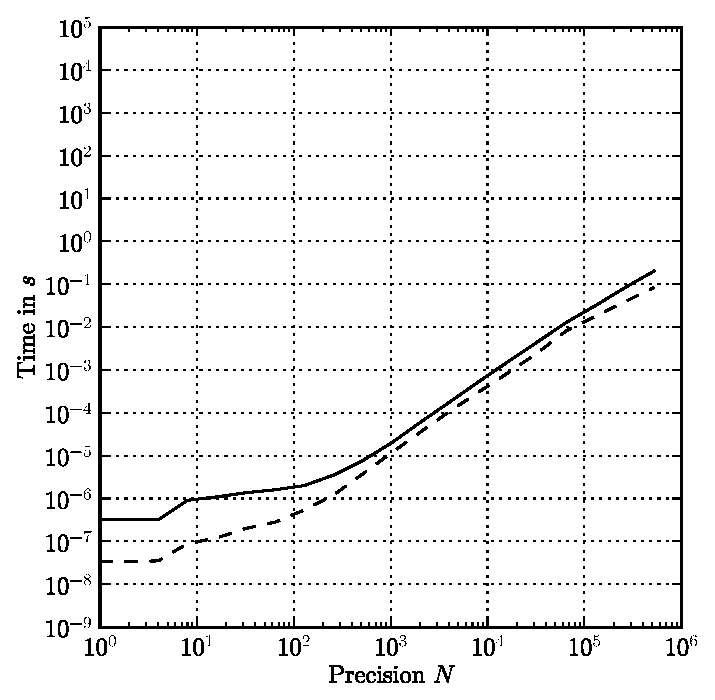
\includegraphics[width=0.84\textwidth]{bin/qp-mul}
\end{minipage}
\begin{minipage}[t]{0.5\linewidth}
\centering
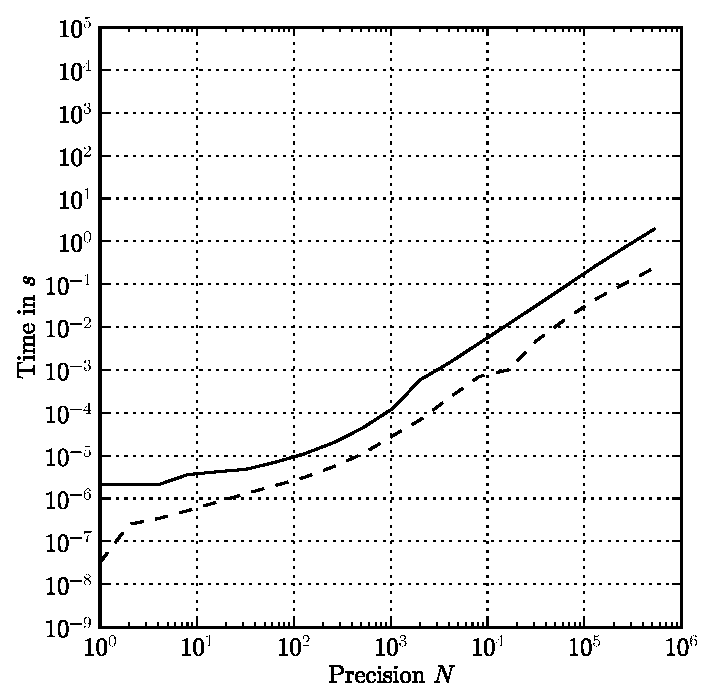
\includegraphics[width=0.84\textwidth]{bin/qp-inv}
\end{minipage}\\

\begin{minipage}[t]{0.5\linewidth}
\centering
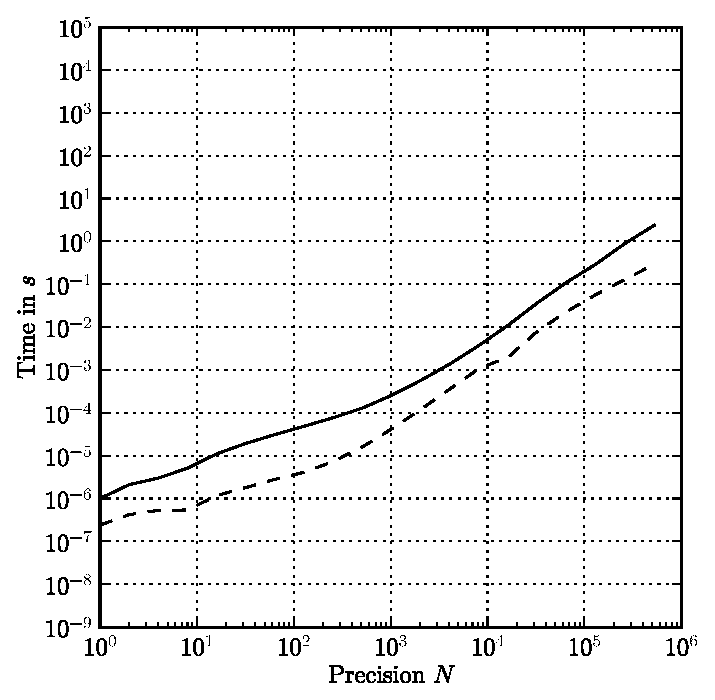
\includegraphics[width=0.84\textwidth]{bin/qp-sqrt}
\end{minipage}
\begin{minipage}[t]{0.5\linewidth}
\centering
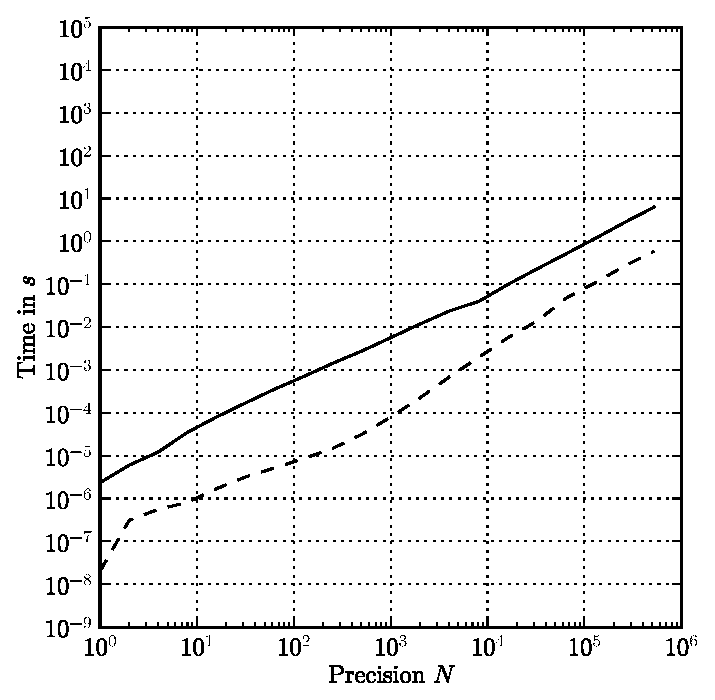
\includegraphics[width=0.84\textwidth]{bin/qp-teichmuller}
\end{minipage}\\

\begin{minipage}[b]{0.5\linewidth}
\centering
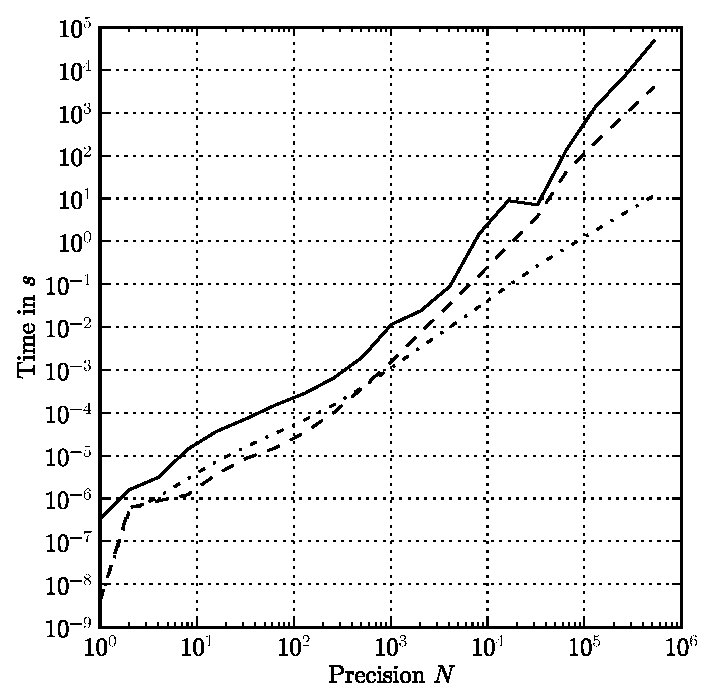
\includegraphics[width=0.84\textwidth]{bin/qp-exp}
\end{minipage}
\begin{minipage}[b]{0.5\linewidth}
\centering
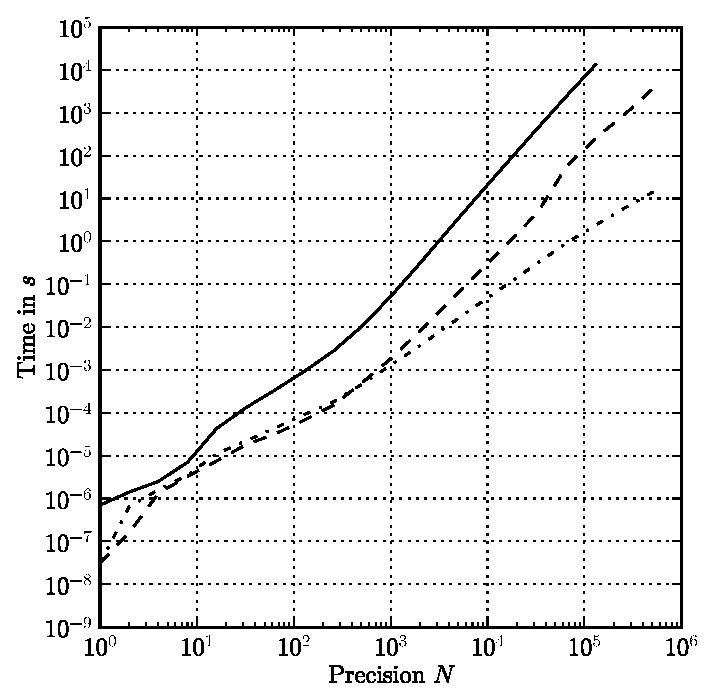
\includegraphics[width=0.84\textwidth]{bin/qp-log}
\end{minipage}
\caption{From left to right, top to bottom, we compute 
$3^{3N} \times 5^{3N}$, $\bigl(3^{3N}\bigr)^{-1}$, $\sqrt{3^{6 N}}$, 
the Teichm\"uller lift of~$3$, $\exp\bigl(17 \times 3^{3N}\bigr)$, and 
$\log\bigl(1 + 17 \times 3^{3N}\bigr)$ modulo $17^N$.  The solid 
lines represent the routines in {\sc Magma}, the dashed and dotted 
lines the routines in {\sc FLINT}.}
\label{fig:timings-qp}
\end{figure}

\begin{figure}[ht]
\begin{minipage}[t]{0.5\linewidth}
\centering
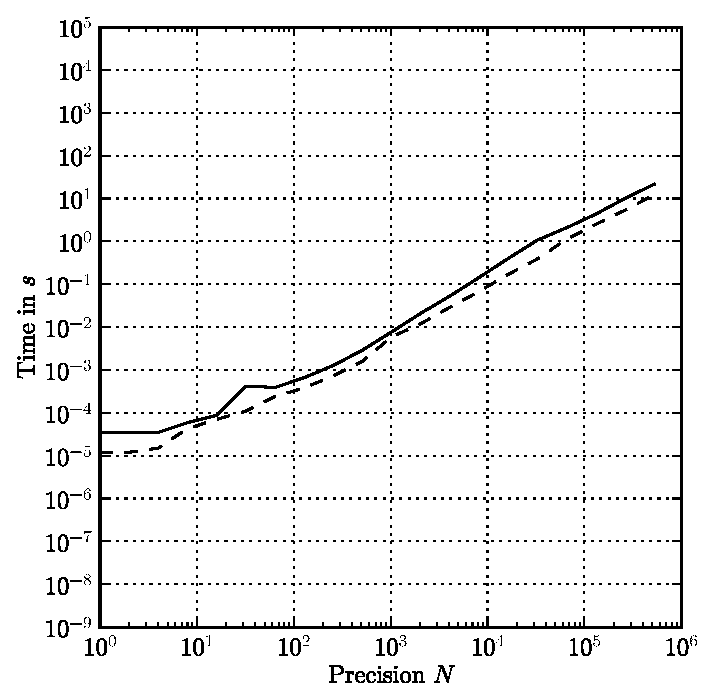
\includegraphics[width=0.84\textwidth]{bin/qq-mul}
\end{minipage}
\begin{minipage}[t]{0.5\linewidth}
\centering
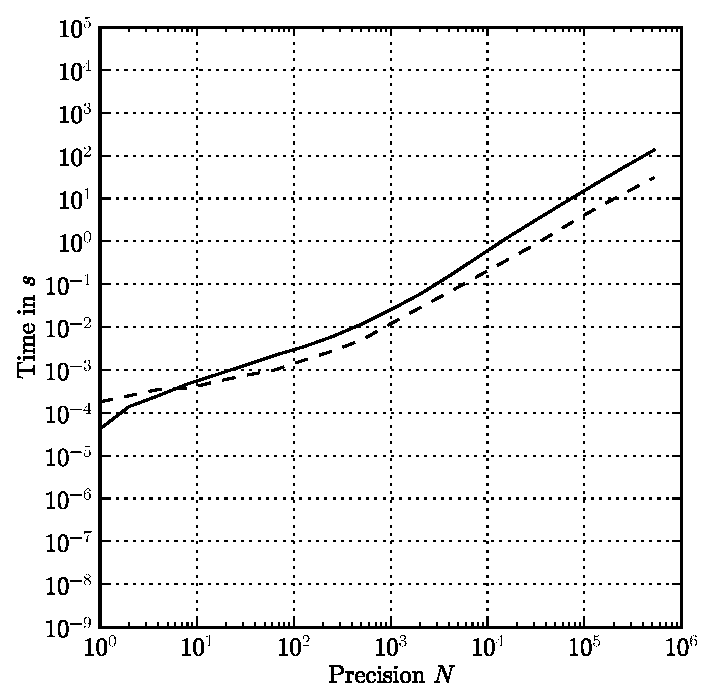
\includegraphics[width=0.84\textwidth]{bin/qq-inv}
\end{minipage}\\

\begin{minipage}[t]{0.5\linewidth}
\centering
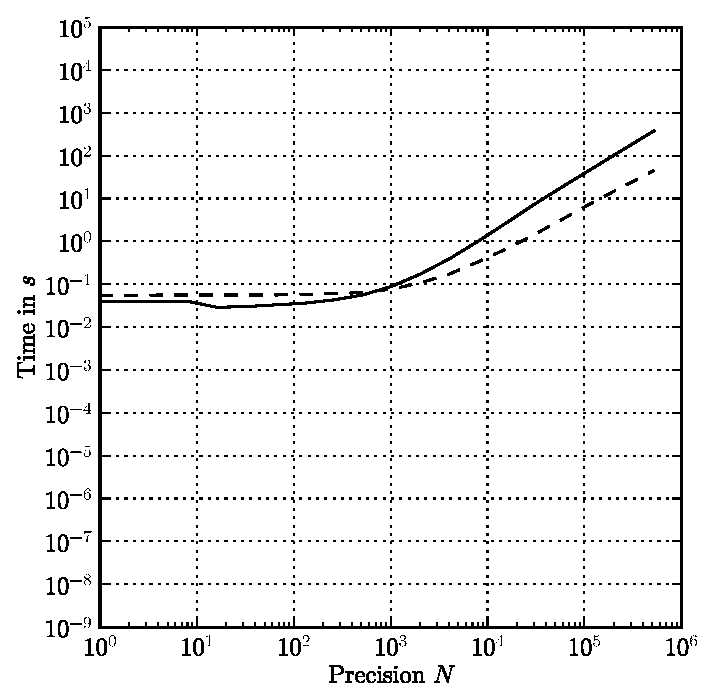
\includegraphics[width=0.84\textwidth]{bin/qq-sqrt}
\end{minipage}
\begin{minipage}[t]{0.5\linewidth}
\centering
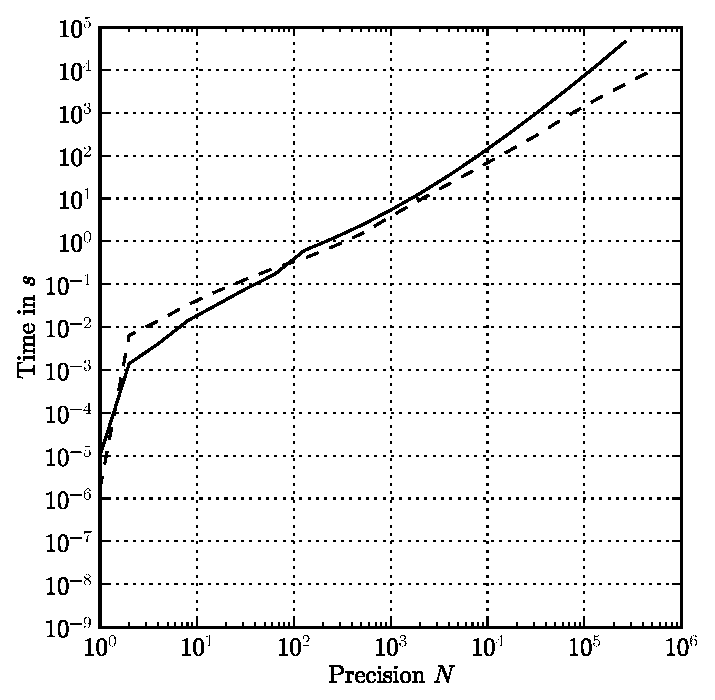
\includegraphics[width=0.84\textwidth]{bin/qq-teichmuller}
\end{minipage}\\

\begin{minipage}[b]{0.5\linewidth}
\centering
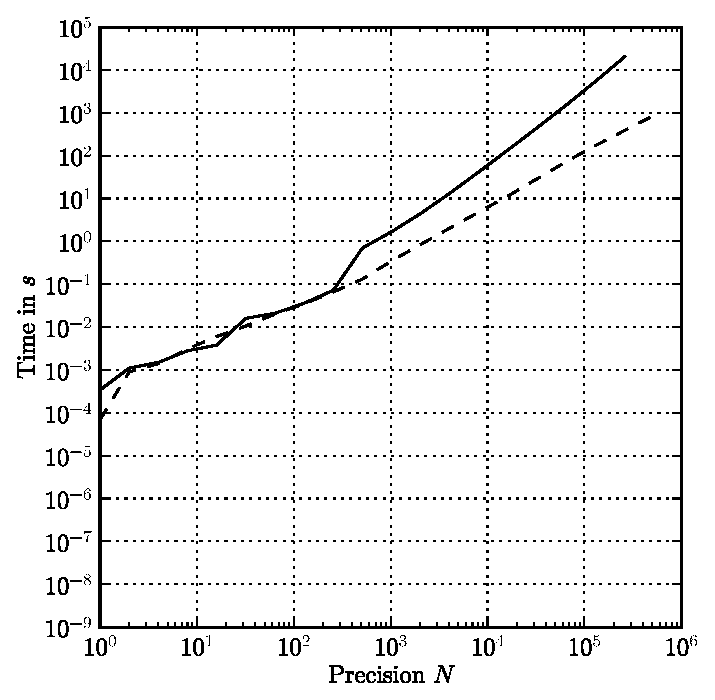
\includegraphics[width=0.84\textwidth]{bin/qq-frobenius}
\end{minipage}
\begin{minipage}[b]{0.5\linewidth}
\centering
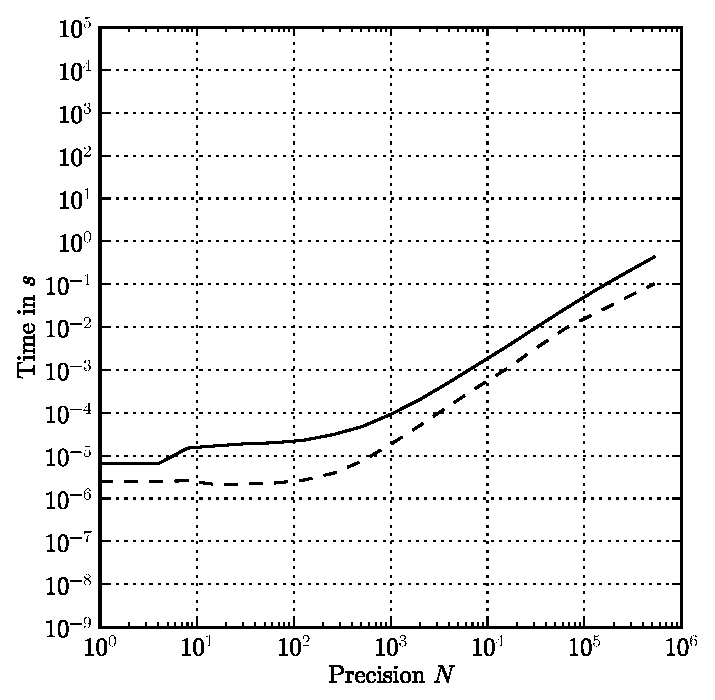
\includegraphics[width=0.84\textwidth]{bin/qq-trace}
\end{minipage}
\caption{From left to right, top to bottom, we compute 
$a \times b$, $a^{-1}$, $\sqrt{a^2}$, the Teichm\"uller lift of~$c$, 
the Frobenius image of~$a$, and the trace of~$a$ in $\Z_{17^{97}}$ 
modulo $17^N$, where $a = \sum (3+i)^{3N} X^i$, $b = \sum (5+2i)^{3N} X^i$, 
and $c = \sum (3+i) X^i \bmod p$.
The solid lines represent the routines in {\sc Magma}, the dashed 
and dotted lines the routines in {\sc FLINT}.}
\label{fig:timings-qq1}
\end{figure}

\begin{figure}[ht]
\begin{minipage}[b]{0.5\linewidth}
\centering
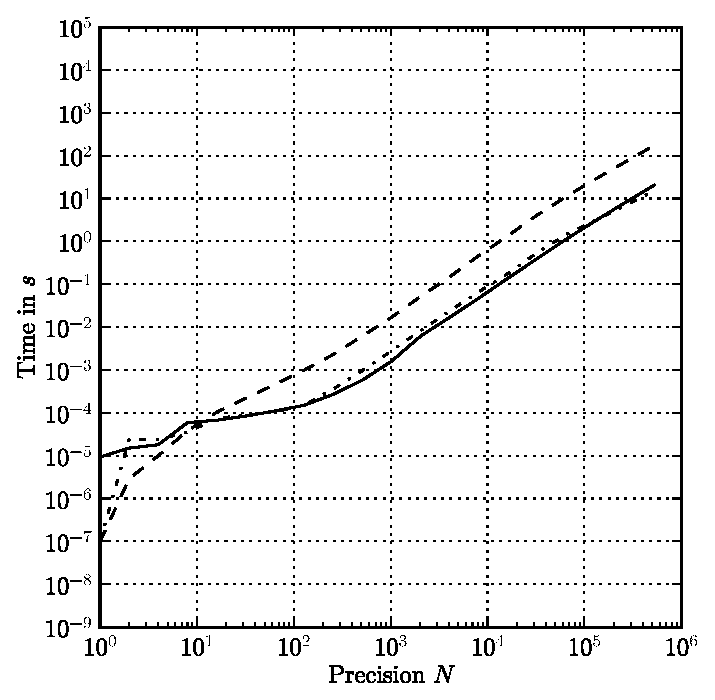
\includegraphics[width=0.84\textwidth]{bin/qq-norm_d5}
\end{minipage}
\begin{minipage}[b]{0.5\linewidth}
\centering
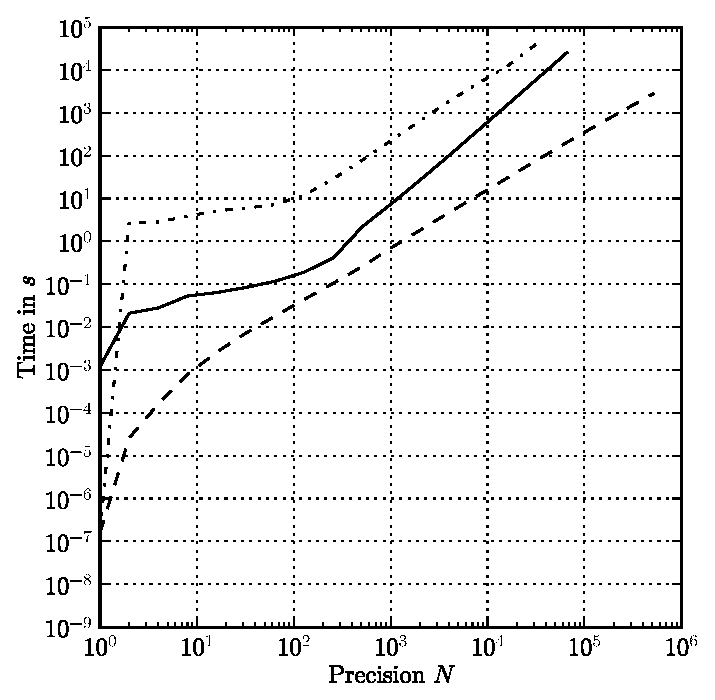
\includegraphics[width=0.84\textwidth]{bin/qq-norm_d97}
\end{minipage}\\

\begin{minipage}[b]{0.5\linewidth}
\centering
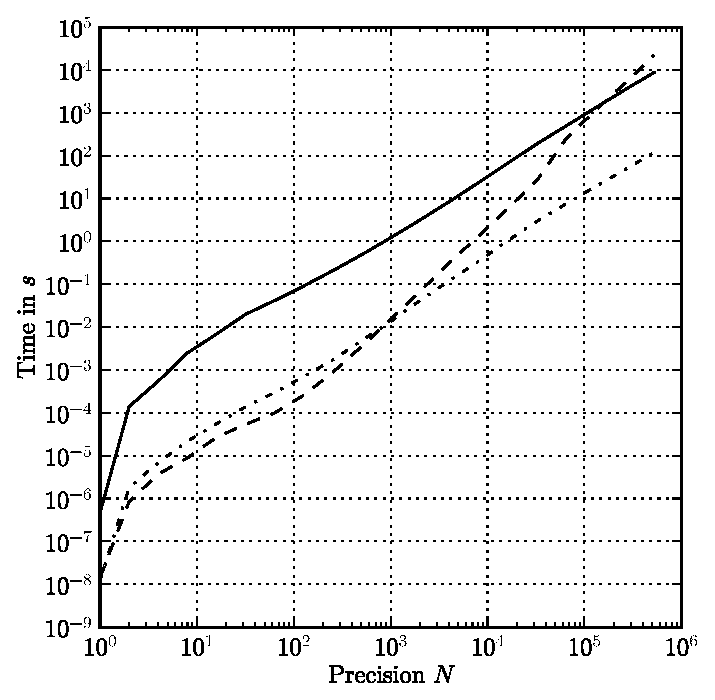
\includegraphics[width=0.84\textwidth]{bin/qq-exp}
\end{minipage}
\begin{minipage}[b]{0.5\linewidth}
\centering
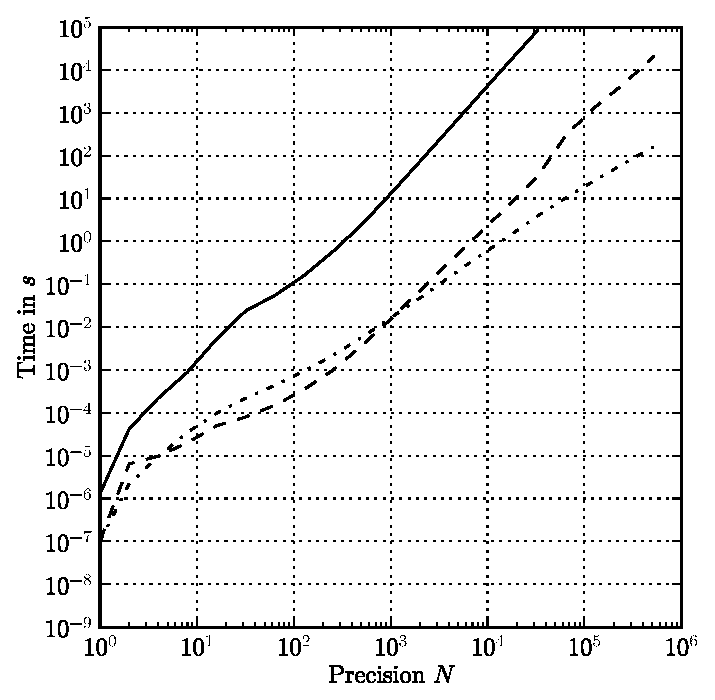
\includegraphics[width=0.84\textwidth]{bin/qq-log}
\end{minipage}
\caption{From left to right, top to bottom, we compute the norm 
of $a$ in $\mathbf{Q}_{17^{5}}$ and $\mathbf{Q}_{17^{97}}$, and 
the exponential of $17 a$ and the logarithm of $1 + 17a$ in 
$\mathbf{Q}_{17^{97}}$, where $a = \sum (3+i)^{3N} X^i$.
The solid lines represent the routines in {\sc Magma}, the dashed 
and dotted lines the routines in {\sc FLINT}.}
\label{fig:timings-qq2}
\end{figure}




}

\backmatter

\phantomsection
\addcontentsline{toc}{chapter}{References}

\bibliographystyle{amsplain}
\bibliography{../SPancratz}

\end{document}

